\documentclass[11pt,a4paper]{article}

\usepackage[margin=2.2cm]{geometry}
\usepackage[T1]{fontenc}
\usepackage[utf8]{inputenc}
\usepackage{lmodern}
\usepackage{microtype}
\usepackage{amsmath,amssymb}
\usepackage{graphicx}
\usepackage{booktabs,array}
\usepackage{enumitem}
\usepackage{xcolor}
\usepackage{listings}
\usepackage{caption}
\usepackage{float}
\usepackage[most]{tcolorbox}
\usepackage{fancyhdr}
\usepackage[hidelinks]{hyperref}

\definecolor{markred}{RGB}{217,13,13}
\definecolor{codebg}{RGB}{245,245,245}

\newcommand{\btn}[1]{\fbox{\small\textsf{#1}}}                 % a button of the GUI
\newcommand{\ctl}[1]{\textsf{#1}}                              % a slider / toggle label
\newcommand{\step}[1]{\tikz[baseline=(c.base)]\node[circle,fill=markred,text=white,inner sep=1.2pt,font=\bfseries\small](c){#1};}
\newcommand{\file}[1]{\texttt{#1}}

\usepackage{tikz}

\newtcolorbox{tryit}{colback=blue!3,colframe=blue!45!black,title=Things to try,fonttitle=\bfseries,
  left=4pt,right=4pt,top=3pt,bottom=3pt}
\newtcolorbox{note}{colback=yellow!6,colframe=orange!70!black,title=Note,fonttitle=\bfseries,
  left=4pt,right=4pt,top=3pt,bottom=3pt}

\lstdefinelanguage{julia}{
  morekeywords={function,end,for,in,if,else,elseif,return,using,const,struct,include,let,do},
  sensitive=true, morecomment=[l]{\#}, morestring=[b]"}
\lstset{language=julia, basicstyle=\ttfamily\small, backgroundcolor=\color{codebg},
  keywordstyle=\color{blue!60!black}\bfseries, commentstyle=\color{green!40!black},
  stringstyle=\color{red!60!black}, frame=single, rulecolor=\color{black!20},
  columns=fullflexible, keepspaces=true, showstringspaces=false, xleftmargin=4pt, xrightmargin=4pt,
  literate={α}{{$\alpha$}}1 {μ}{{$\mu$}}1 {–}{{--}}1}

\pagestyle{fancy}
\fancyhf{}
\lhead{\small Interactive phase equilibria with Julia}
\rhead{\small\thepage}
\renewcommand{\headrulewidth}{0.3pt}

\setlist{itemsep=2pt,topsep=4pt}
\captionsetup{font=small,labelfont=bf}

\title{\textbf{Interactive phase equilibria with Julia}\\[4pt]
\large A guide to the example programs: Gibbs energy, linear programming\\ and seven interactive examples}
\author{Evangelos Moulas\\[2pt] {\small (made using Claude)}}
\date{Version 1.4 -- 23 Nov.\ 2026}

\begin{document}
\maketitle
\vspace{-3ex}
\thispagestyle{empty}

\begin{abstract}
\noindent This guide explains how to install and run the interactive Julia programs of the course and what
they compute. All programs do the same thing: for given pressure, temperature and bulk composition they find
the stable mineral assemblage by \emph{minimising the Gibbs energy of the system}, written as a linear
programme. Section~\ref{sec:intro} tells you how to start the programs, Section~\ref{sec:gibbs} how the Gibbs
energy of every phase is calculated and Section~\ref{sec:lp} how the minimisation is set up. The calculation
is always done in moles; the diagrams of Examples 2–6 are \emph{shown} in weight per cent, like the published
diagrams they are compared with (Section~\ref{sec:weight}). Sections
\ref{sec:ex0}–\ref{sec:ex6} then go through the seven examples one by one. Every example has an annotated
screenshot: the red numbers \step{1}, \step{2}, \dots\ show where to click and in which order.
\end{abstract}

\vspace{-2ex}
\tableofcontents
\newpage

%==============================================================================
\section{Introduction and installation}\label{sec:intro}
%==============================================================================

\subsection{What the programs do}
A mineral assemblage at equilibrium is the combination of phases (and phase compositions) that has the
lowest total Gibbs energy $G$ at the given pressure $P$, temperature $T$ and bulk composition. The programs
let you \emph{see} this minimisation: they draw the Gibbs energy $g$ of every phase as a function of
composition (the $g$–$x$ diagram) and the phase diagram that results from minimising $G$ at many $P$, $T$
or compositions. You can click a point in the phase diagram and immediately see the $g$–$x$ diagram that
explains why that assemblage is stable.

\begin{table}[H]
\centering\footnotesize
\caption{The example programs. All of them are in the main folder.}\label{tab:files}
\begin{tabular}{@{}ll>{\raggedright\arraybackslash}p{6.9cm}@{}}
\toprule
File & Diagram & Topic \\
\midrule
\file{Example0\_fixed\_composition.jl}   & $P$–$T$       & three phases of fixed composition, a univariant reaction \\
\file{Example1\_solution\_playground.jl} & $g$–$x$       & solid solution, solvus, compounds, melt; switch phases on/off \\
\file{Example2\_eutectic\_TX.jl}         & $T$–$X$       & binary eutectic Di–An \\
\file{Example3\_peritectic\_TX.jl}       & $T$–$X$       & binary peritectic Fo–SiO$_2$ (En melts incongruently; two liquids) \\
\file{Example4\_olivine\_loop\_TX.jl}    & $T$–$X$       & melting loop of a solid solution (olivine Fo–Fa) \\
\file{Example5\_ternary\_DiAnFo.jl}      & ternary       & Di–An–Fo, calibrated against the liquidus diagram \\
\file{Example6\_ternary\_CAS.jl}         & ternary       & CaO–Al$_2$O$_3$–SiO$_2$: 13 solids (congruent and incongruent compounds), calibrated against the liquidus projection \\
\midrule
\file{gibbs\_lp.jl}                      & --            & the common core: Gibbs energies and the linear programme \\
\file{window\_size.jl}                   & --            & makes the window smaller at start-up if the screen is small \\
\file{Project.toml}                      & --            & the Julia environment (list of packages) \\
\file{data/olivine\_1bar\_experiments.csv} & --          & experimental data for Example 4 \\
\file{data/DiAn\_liquidus\_digitized.txt} & --           & digitised Di–An liquidus (fit of Ex.~2) \\
\file{data/FoSiO2\_liquidus\_Morse\_digitized.txt} & --  & digitised Fo–SiO$_2$ diagram (fit of Ex.~3) \\
\file{data/FoSiO2\_liquidus\_digitized.txt} & --         & earlier Fo–SiO$_2$ digitisation (not used) \\
\file{data/CAS\_liquidus\_digitized.txt} & --            & digitised CaO–Al$_2$O$_3$–SiO$_2$ projection (fit of Ex.~6) \\
\file{data/Papers/}                      & --            & source papers (MgO–FeO–SiO$_2$; Di–Fo–An; MgO–Al$_2$O$_3$–SiO$_2$), the olivine loop figure and the CaO–Al$_2$O$_3$–SiO$_2$ liquidus projection \\
\file{calibration/}                      & --            & the programs that fit the melt models of Examples 2, 3 and 6 \\
\file{guide/}                            & --            & this guide and the program that makes its screenshots \\
\bottomrule
\end{tabular}
\end{table}

\subsection{Installation (once)}
\begin{enumerate}
\item Install a recent Julia from \url{https://julialang.org/downloads/} (the programs were developed with
  Julia 1.13). The recommended
  installer is \emph{juliaup}; on macOS/Linux type
  \lstinline{curl -fsSL https://install.julialang.org | sh} in a terminal, on Windows install
  \emph{Julia} from the Microsoft Store.
\item Copy (or \texttt{git clone}) the folder with the programs to your computer.
\item Open a terminal in that folder and install the packages listed in \file{Project.toml}
  (GLMakie for the graphics, JuMP and GLPK for the linear programme):
\begin{lstlisting}
julia --project=. -e "using Pkg; Pkg.instantiate()"
\end{lstlisting}
  This downloads and precompiles the packages and takes several minutes the first time. No
  \file{Manifest.toml} is included, so the latest compatible versions are installed and a
  \file{Manifest.toml} is written in the folder.
\end{enumerate}

\subsection{Running an example}
From a terminal in the main folder:
\begin{lstlisting}
julia Example0_fixed_composition.jl
\end{lstlisting}
A window opens; the program runs until you close the window. Every script activates the project by itself
(\lstinline{Pkg.activate(@__DIR__)}), so no extra options are needed. Alternatively, start Julia and use the
REPL (this is also how it works inside VS Code):
\begin{lstlisting}
julia> include("Example0_fixed_composition.jl")   # opens the window; defines fig and app
\end{lstlisting}

\begin{note}
The first start of a session takes a while (typically 30–60\,s): Julia compiles the graphics and the solver.
Afterwards the programs react immediately. If no window appears, your computer needs working OpenGL drivers
(GLMakie); this is usually not available on remote or headless machines.
\end{note}

\subsection{Elements of the user interface}
All windows use the same few elements:
\begin{itemize}
\item \textbf{The window} opens with at most 85\,\% of the width and 80\,\% of the height of the screen, so
  that it fits on a small screen as well (the figures are designed for about $1500 \times 950$). Text and
  controls keep their size; the diagrams get the space that is left. The limits can be changed in
  \file{window\_size.jl} (\lstinline{WINDOW_FRACTION}).
\item \textbf{Diagrams}: a \emph{left click} in a phase diagram picks a point (a cross appears). Zooming and
  panning are switched off so that the diagrams do not move by accident (the 3D views of Examples~5 and~6
  can be rotated by dragging; the $T$–$X$ diagram of Example~3 has its own zoom, Section~\ref{sec:ex3}).
\item \textbf{Buttons}, e.g.\ \btn{Compute g–x}: click once.
\item \textbf{Sliders}: drag the knob; the value is shown on the right.
\item \textbf{Toggles} (round switches) and \textbf{check boxes}: click to switch on/off.
\item \textbf{Status lines} (grey text below the controls): what was computed, how many linear programmes were
  solved and how long it took; the \emph{cursor} line shows the stable assemblage under the mouse.
\end{itemize}
Every program has a \textbf{USER INPUT} block at the top of the file. This is the place to change the
thermodynamic data (energies, entropies, volumes, melting points, Margules parameters) and the ranges of the
diagrams. Save the file and run it again.

%==============================================================================
\section{How the Gibbs energy is calculated}\label{sec:gibbs}
%==============================================================================

\subsection{Phases of fixed composition}
For a phase of fixed composition, $\mathrm{d}g = -s\,\mathrm{d}T + v\,\mathrm{d}P$. If the entropy $s$ and the
volume $v$ are taken as constants (no heat capacity, no compressibility or thermal expansion), integration
gives a plane in $P$–$T$:
\begin{equation}\label{eq:g}
  g(P,T) = g_0 - s\,T + v\,P .
\end{equation}
Every phase in the programs is described by the three numbers $(g_0, s, v)$ and by its composition (the
amounts of the components in moles, e.g.\ \lstinline{[0.5, 0.5]} for AB). Units: $g$ in kJ/mol, $s$ in kJ/(mol\,K),
$v$ in kJ/(kbar\,mol), $T$ in K, $P$ in kbar; note that 1\,kJ/kbar = 10\,cm$^3$.
Equation~\eqref{eq:g} is implemented in \file{gibbs\_lp.jl} as \lstinline{gibbs(p, P, T)}.

\subsection{Melts from melting data}
The Gibbs energy of a pure melt is written relative to the solid of the same composition. With the enthalpy
of fusion $\Delta H$, the melting point $T_m$ and the volume of fusion $\Delta V$:
\begin{equation}\label{eq:melt}
  g^{\,l} - g^{\,s} = \Delta H \left(1 - \frac{T}{T_m}\right) + \Delta V\,P ,
  \qquad \Delta S = \frac{\Delta H}{T_m},\qquad \frac{\mathrm{d}T_m}{\mathrm{d}P} = \frac{\Delta V}{\Delta S}.
\end{equation}
This is again of the form \eqref{eq:g}: $g_0^{\,l} = g_0^{\,s} + \Delta H$, $s^l = s^s + \Delta H/T_m$,
$v^l = v^s + \Delta V$. The melt is more stable than the solid above $T_m$ and less stable below it.

\subsection{Solutions}
A binary solution of the end-members 1 and 2 (composition $X = X_2$, the \emph{mole} fraction of
end-member 2) has
\begin{equation}\label{eq:sol}
\begin{aligned}
  g(X) &= (1-X)\,g_1 + X\,g_2 + n R T\left[X\ln X + (1-X)\ln(1-X)\right] + W\,X(1-X),\\
  W &= W_H - T\,W_S + P\,W_V .
\end{aligned}
\end{equation}
The first two terms are the mechanical mixture, the third is the ideal (configurational) entropy of mixing
on $n$ sites per formula unit, the last one the excess (regular-solution or Margules) term. With $W=0$ the
solution is ideal. If $W > 2nRT$ the curve $g(X)$ gets a hump and the solution separates into two phases
(a \emph{solvus}); the top of the solvus is at $T_c = W/(2nR)$. The chemical potentials of the end-members,
i.e.\ the intercepts of the tangent to $g(X)$ at $X$, are
\begin{equation}\label{eq:mu}
  \mu_1 = g_1 + nRT\ln(1-X) + W X^2,\qquad \mu_2 = g_2 + nRT\ln X + W(1-X)^2 .
\end{equation}

\paragraph{Pseudocompounds.} For a \emph{fixed} $X$, Eq.~\eqref{eq:sol} is again linear in $T$ and $P$, i.e.\ of
the form \eqref{eq:g}: the mixing entropy simply adds to $s$. The programs therefore replace the continuous
curve by many phases of fixed composition at $X = 0, \tfrac{1}{n-1}, \dots, 1$, the so-called
\emph{pseudocompounds} (\lstinline{solution_pseudocompounds} in \file{gibbs\_lp.jl}; by default 201 per
solution in Examples 1, 2 and 4). Example~3 uses its own liquid model and spaces its 201 liquids evenly on
the wt\% axis instead; Examples~5 and~6 place the liquid on a triangular grid with a step of $1/n$ in weight
fraction ($n = 40$ by default, i.e.\ 861 pseudocompounds).
This turns every problem into the same kind of problem as for pure phases.

\paragraph{More than one excess term.} A single $W$ gives an excess term that is symmetric about $X = 0.5$.
Example~3 needs an asymmetric melt and uses three terms of the same kind (a Redlich–Kister series),
\begin{equation}\label{eq:rk}
  g^{\,ex} = X(1-X)\sum_{k=0}^{2} \left(a_k - b_k T\right)(1-2X)^k ,
\end{equation}
of which the first one ($k=0$) is the regular solution with $W = a_0 - b_0 T$. For a fixed $X$ this is again
linear in $T$, so the pseudocompounds work in the same way.

\subsection{Moles in the calculation, weight per cent in the plots}\label{sec:weight}
All Gibbs energies above are per mole and all compositions are mole fractions: the ideal entropy of mixing in
Eq.~\eqref{eq:sol} counts particles, not grams. The published phase diagrams that Examples 2–6 are compared
with are, however, drawn in \emph{weight} per cent. The programs therefore calculate in moles and convert
only what is \emph{shown}. For a phase with the mole fractions $x_i$ of the components, whose molar masses
are $M_i$ (Table~\ref{tab:mass}), the mass of one mole is $\bar M = \sum_i x_i M_i$ and
\begin{equation}\label{eq:wt}
  w_i = \frac{x_i M_i}{\bar M}, \qquad
  x_i = \frac{w_i/M_i}{\sum_j w_j/M_j}, \qquad
  g\,[\mathrm{J/g}] = \frac{g\,[\mathrm{J/mol}]}{\bar M}, \qquad
  \mu_i\,[\mathrm{J/g}] = \frac{\mu_i\,[\mathrm{J/mol}]}{M_i} .
\end{equation}
Three consequences are used in Examples 2–6:
\begin{itemize}
\item \textbf{The common tangent stays straight.} Dividing the tangent line $g = \sum_i \mu_i x_i$ by $\bar M$
  gives $g/\bar M = \sum_i (\mu_i/M_i)\,w_i$: a straight line (a plane in the ternary) in mole fractions and
  energy per mole is also a straight line in weight fractions and energy \emph{per gram}. The $g$–$x$
  diagrams are therefore drawn as $g$ in J/g against wt\%. The intercepts of the tangent are the chemical
  potentials per gram; the molar values in kJ/mol are printed next to them.
\item \textbf{The lever rule gives mass fractions.} The amounts $\alpha_i$ that the linear programme returns
  are moles. In a wt\% diagram the lever rule gives mass fractions,
  $\alpha_i \bar M_i / \sum_j \alpha_j \bar M_j$; these are the amounts that are printed (in wt\%).
\item \textbf{The numbers differ.} The Di–An eutectic lies at 42\,wt\% An but at 36\,mol\% An; enstatite has
  59.85\,wt\% SiO$_2$ but lies at 50\,mol\% SiO$_2$ between Mg$_2$SiO$_4$ and SiO$_2$. A diagram that is read
  in the wrong unit gives wrong thermodynamic parameters.
\end{itemize}

\begin{table}[H]
\centering\small
\caption{Molar masses used for the conversion (g/mol).}\label{tab:mass}
\begin{tabular}{@{}lllllll@{}}
\toprule
Di, CaMgSi$_2$O$_6$ & An, CaAl$_2$Si$_2$O$_8$ & Fo, Mg$_2$SiO$_4$ & Fa, Fe$_2$SiO$_4$ & SiO$_2$ & CaO & Al$_2$O$_3$ \\
\midrule
216.55 & 278.21 & 140.69 & 203.77 & 60.08 & 56.08 & 101.96 \\
\bottomrule
\end{tabular}
\end{table}

\paragraph{Calibrated examples.} Examples 2, 3, 5 and 6 reproduce published diagrams. Their curves were read off
the diagrams in wt\%, \emph{converted to mole fractions}, and the parameters of the melt (enthalpies of fusion,
excess terms) were fitted to them in mole fractions. The fitted numbers are parameters of these simple models,
not calorimetric values. For Examples 2, 3 and 6 the digitised curves are in the folder \file{data/} and the
programs that do the fit in \file{calibration/}; they can be run again, e.g.\
\lstinline{julia calibration/fit_Example2_DiAn.jl}. Example 5 (ternary) uses the same ideas with three
end-members, an effective number of mixing units per formula unit and asymmetric excess terms
(Section~\ref{sec:ex5}); Example 6 extends them to a ternary of oxides with thirteen compounds
(Section~\ref{sec:ex6}).

%==============================================================================
\section{How the minimisation is set up}\label{sec:lp}
%==============================================================================

\subsection{The linear programme}
Let phase $i$ have the Gibbs energy $g_i(P,T)$ per mole and the (normalised) composition $A_{ji}$, the mole
fraction of component $j$ in phase $i$ (the columns of the matrix $A$ sum to one). The unknowns are the
amounts $\alpha_i$ of the phases in moles. The stable assemblage at given $P$, $T$ and bulk composition $b_j$ solves
\begin{equation}\label{eq:lp}
\begin{aligned}
  &\min_{\alpha}\ G = \sum_i g_i\,\alpha_i \qquad \text{subject to}\\
  &\sum_i A_{ji}\,\alpha_i = b_j \ \ \text{(mass balance of every component $j$)},\qquad \alpha_i \ge 0 .
\end{aligned}
\end{equation}
Both the objective and the constraints are linear in $\alpha$: this is a \emph{linear programme} (LP). It is
solved with JuMP and the GLPK solver; the model is built once and only the costs $g_i$ (when $P$ or $T$
change) or the right-hand side $b_j$ (when the bulk composition changes) are updated, which makes thousands of
solutions per second possible.

\subsection{What the solution tells us}
\begin{itemize}
\item \textbf{Phase amounts.} The phases with $\alpha_i > 0$ are the stable assemblage; $\alpha_i$ are their
  proportions in moles (the lever rule). Examples 2–6 print them as mass fractions (Section~\ref{sec:weight}).
\item \textbf{Chemical potentials.} The Lagrange multipliers (dual variables) $\mu_j$ of the mass-balance
  constraints are the chemical potentials of the components. The dual problem is
  $\max \sum_j \mu_j b_j$ subject to $\sum_j A_{ji}\mu_j \le g_i$ for every phase: the tangent line (plane)
  $g = \sum_j \mu_j X_j$ lies \emph{below or on} every phase and touches the stable ones. This is the common
  tangent construction of the $g$–$x$ diagrams.
\item \textbf{Phase rule.} An optimal \emph{basic} solution has at most as many non-zero $\alpha_i$ as there are
  constraints, i.e.\ components $c$: at fixed $P$ and $T$ at most $c$ phases coexist. On a reaction line one
  more phase touches the tangent, but the LP still reports $c$ of them; the programs then print
  ``on reaction'' or ``eutectic''.
\item \textbf{Non-unique $\mu$.} If fewer than $c$ phases are stable, the tangent can rotate around them and $\mu$
  is not unique; the programs say so. For a single solution phase they use the tangent to the continuous
  curve, Eq.~\eqref{eq:mu}.
\end{itemize}

\subsection{Solutions in the LP}
With pseudocompounds the LP picks the points of the lower convex hull of all phases. Two \emph{neighbouring}
pseudocompounds of the same solution represent one phase whose composition lies between them; two
separated ones represent two coexisting phases of the same solution (e.g.\ $\alpha + \alpha$ across a
solvus). Examples 2–4 take two stable pseudocompounds that are not neighbours as two phases; Examples 1,
5 and 6 check in addition whether the continuous $g$ curve (surface) between them has a hump.
The composition of a solution phase is resolved to about the spacing of the pseudocompounds; you can change
their number with a slider to see the effect.

\subsection{From single points to phase diagrams}
A phase diagram is obtained by solving the LP on a grid (of $P$–$T$, $T$–$X$ or compositions). Wherever two
neighbouring grid nodes have different assemblages, a field boundary lies between them; it is located by
bisection along that grid edge (black dots in the diagrams). Coloured fields show the assemblage at the grid
nodes. Where an independent (analytic or exact) solution exists, it is drawn as a dashed line so that you can
check the LP. A field that is thinner than the spacing of the grid can fall between the nodes; it is then not
drawn. Use more \ctl{Grid nodes} or, in Example~3, the zoom (Section~\ref{sec:ex3}).

\subsection{Using the core directly}
\file{gibbs\_lp.jl} can be used without the graphics, e.g.\ in the REPL:
\begin{lstlisting}
using Pkg; Pkg.activate(".")
include("gibbs_lp.jl")
phases = [Phase("A",  [1.0, 0.0], 10.0, 0.020, 1.00),     # name, composition, g0, s, v
          Phase("B",  [0.0, 1.0], 14.0, 0.016, 0.80),
          Phase("AB", [0.5, 0.5], 16.0, 0.028, 1.15)]
lp = GibbsLP(phases, [0.75, 0.25])     # bulk composition X_B = 0.25
r  = solve!(lp, 20.0, 500.0)           # P = 20 kbar, T = 500 K
r.stable    # [1, 2]            -> A + B
r.α         # [0.75, 0.25, 0.0]
r.μ         # [20.0, 22.0]      chemical potentials of A and B
\end{lstlisting}

%==============================================================================
\clearpage
\section{Example 0 – three phases of fixed composition (\texorpdfstring{$P$–$T$}{P–T})}\label{sec:ex0}
%==============================================================================
\textbf{File:} \file{Example0\_fixed\_composition.jl}.\quad
\textbf{Phases:} A ($X_B = 0$), AB ($X_B = 0.5$) and B ($X_B = 1$), all of fixed composition.

The reaction $\tfrac12\mathrm{A} + \tfrac12\mathrm{B} = \mathrm{AB}$ has
$\Delta g_0 = 4$\,kJ, $\Delta s = 0.010$\,kJ/K, $\Delta v = 0.25$\,kJ/kbar, so it is the straight line
$P = 0.04\,T - 16$ (dashed): AB is stable at high $T$ and low $P$. At start-up the LP is solved on a
$25\times25$ $P$–$T$ grid and the boundary is located by bisection.

\begin{figure}[H]
\centering
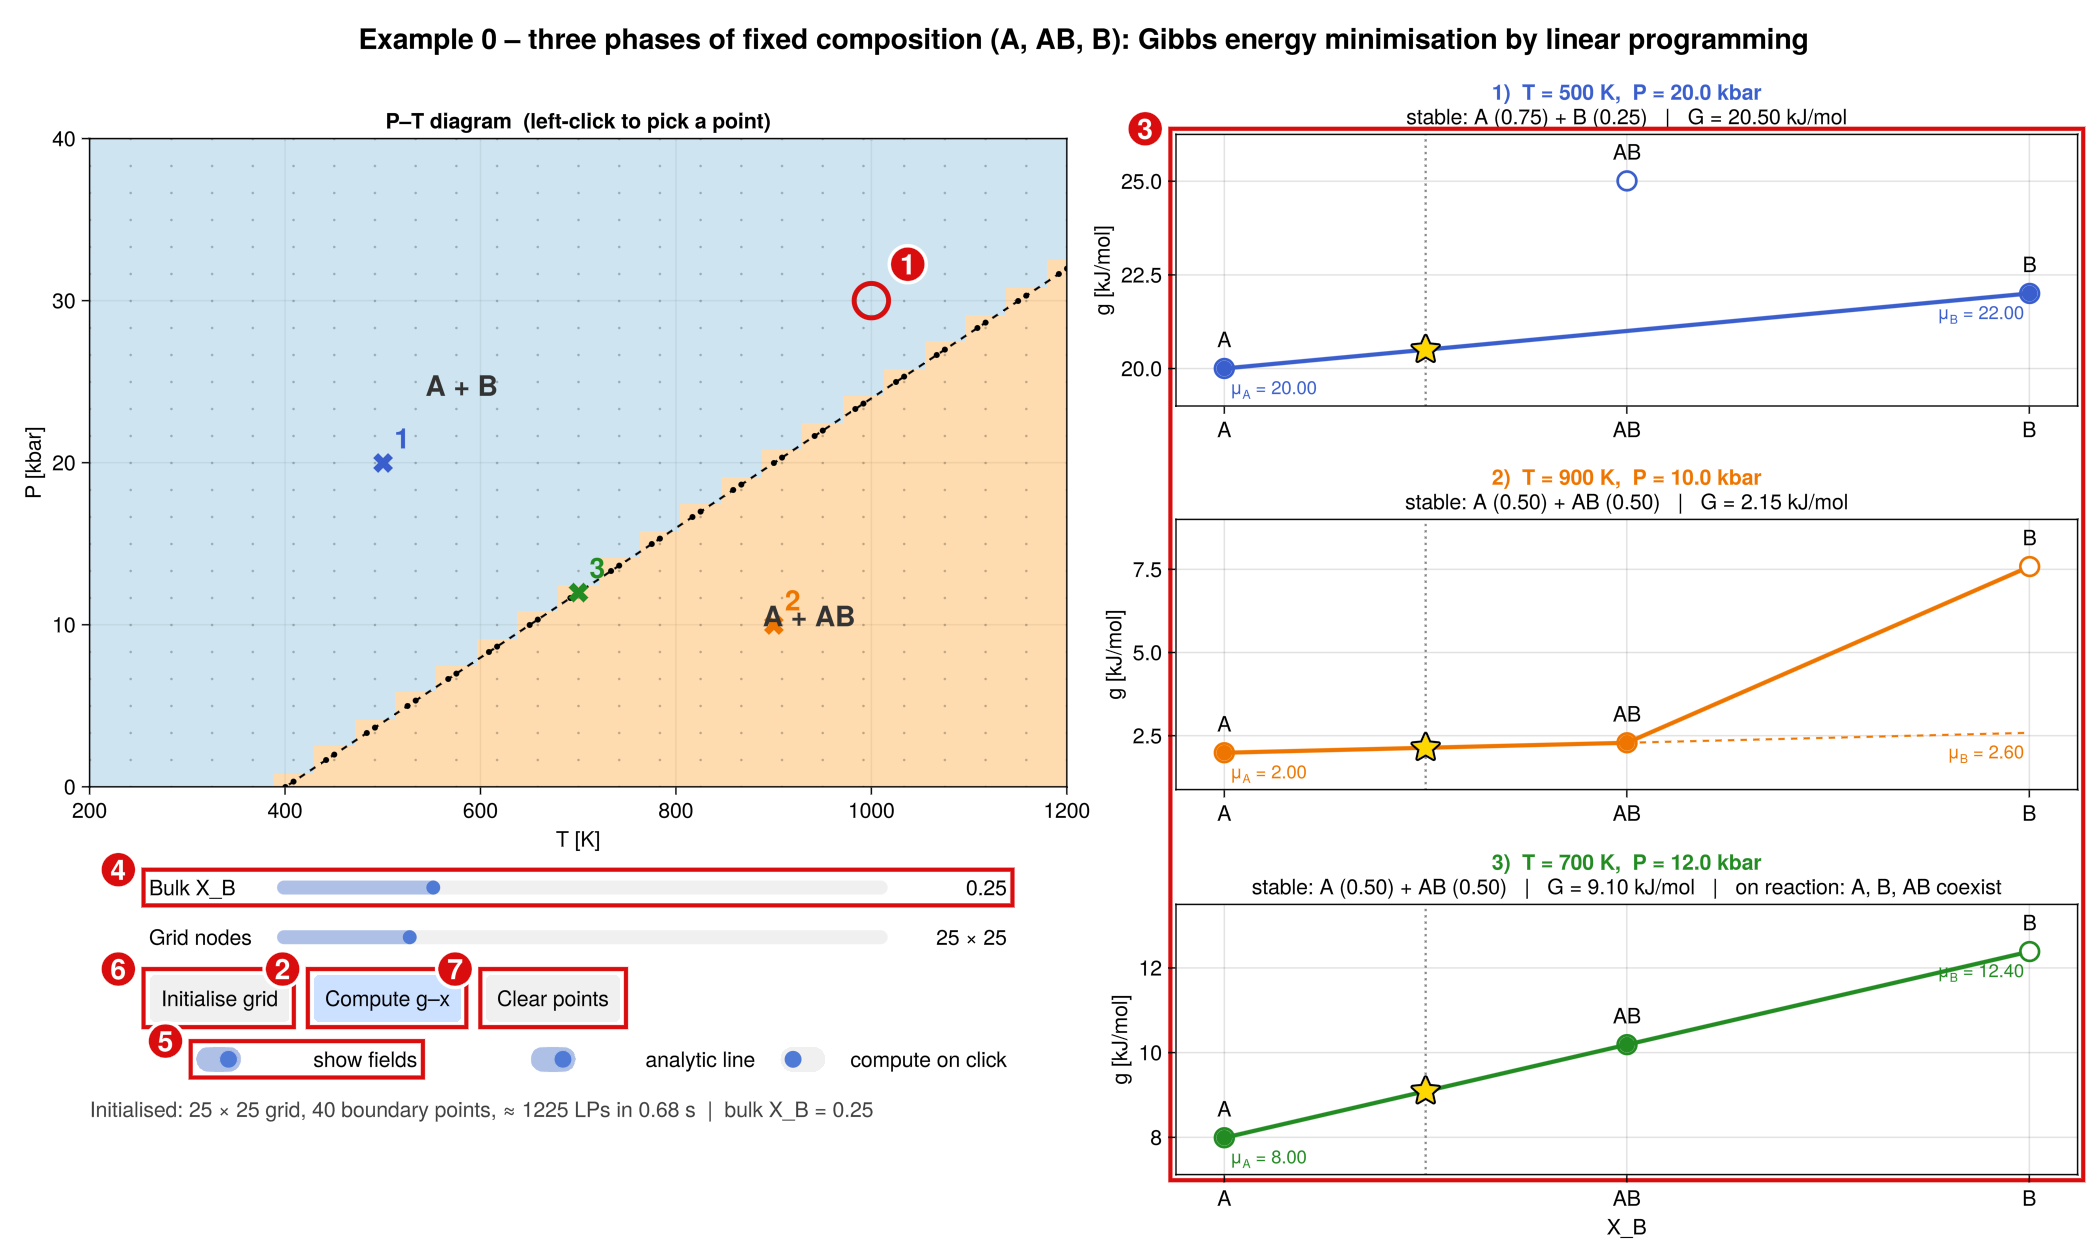
\includegraphics[width=\textwidth]{figures/ex0_overview.png}
\caption{Example 0 after three points have been computed (1: $A+B$, 2: $A+AB$, 3: on the reaction line).}
\label{fig:ex0}
\end{figure}

\paragraph{Step by step} (numbers as in Fig.~\ref{fig:ex0})
\begin{enumerate}[label=\protect\step{\arabic*}]
\item \textbf{Left-click} anywhere in the $P$–$T$ diagram. A black cross marks the point; the status line
  tells you the stable assemblage there.
\item Click \btn{Compute g–x}. The point becomes a numbered, coloured cross.
\item The $g$–$x$ diagram of that point appears in the next free panel on the right (up to three; the
  oldest one is dropped afterwards). Filled circles are stable phases, open circles metastable ones; the
  thick line is the lowest $G$ of the system for every bulk composition (the lower convex hull), the dashed
  line the tangent with its intercepts $\mu_A$ and $\mu_B$, the star the bulk composition.
\item \ctl{Bulk X\_B} changes the bulk composition; the grid and all panels are recomputed.
\item \ctl{show fields} hides the coloured fields (and \ctl{analytic line} the dashed reaction line), so that
  students can first find the topology themselves; \ctl{compute on click} skips step~2.
\item \btn{Initialise grid} recomputes the grid, e.g.\ after changing the number of \ctl{Grid nodes}.
\item \btn{Clear points} empties all panels.
\end{enumerate}

\begin{figure}[H]
\centering
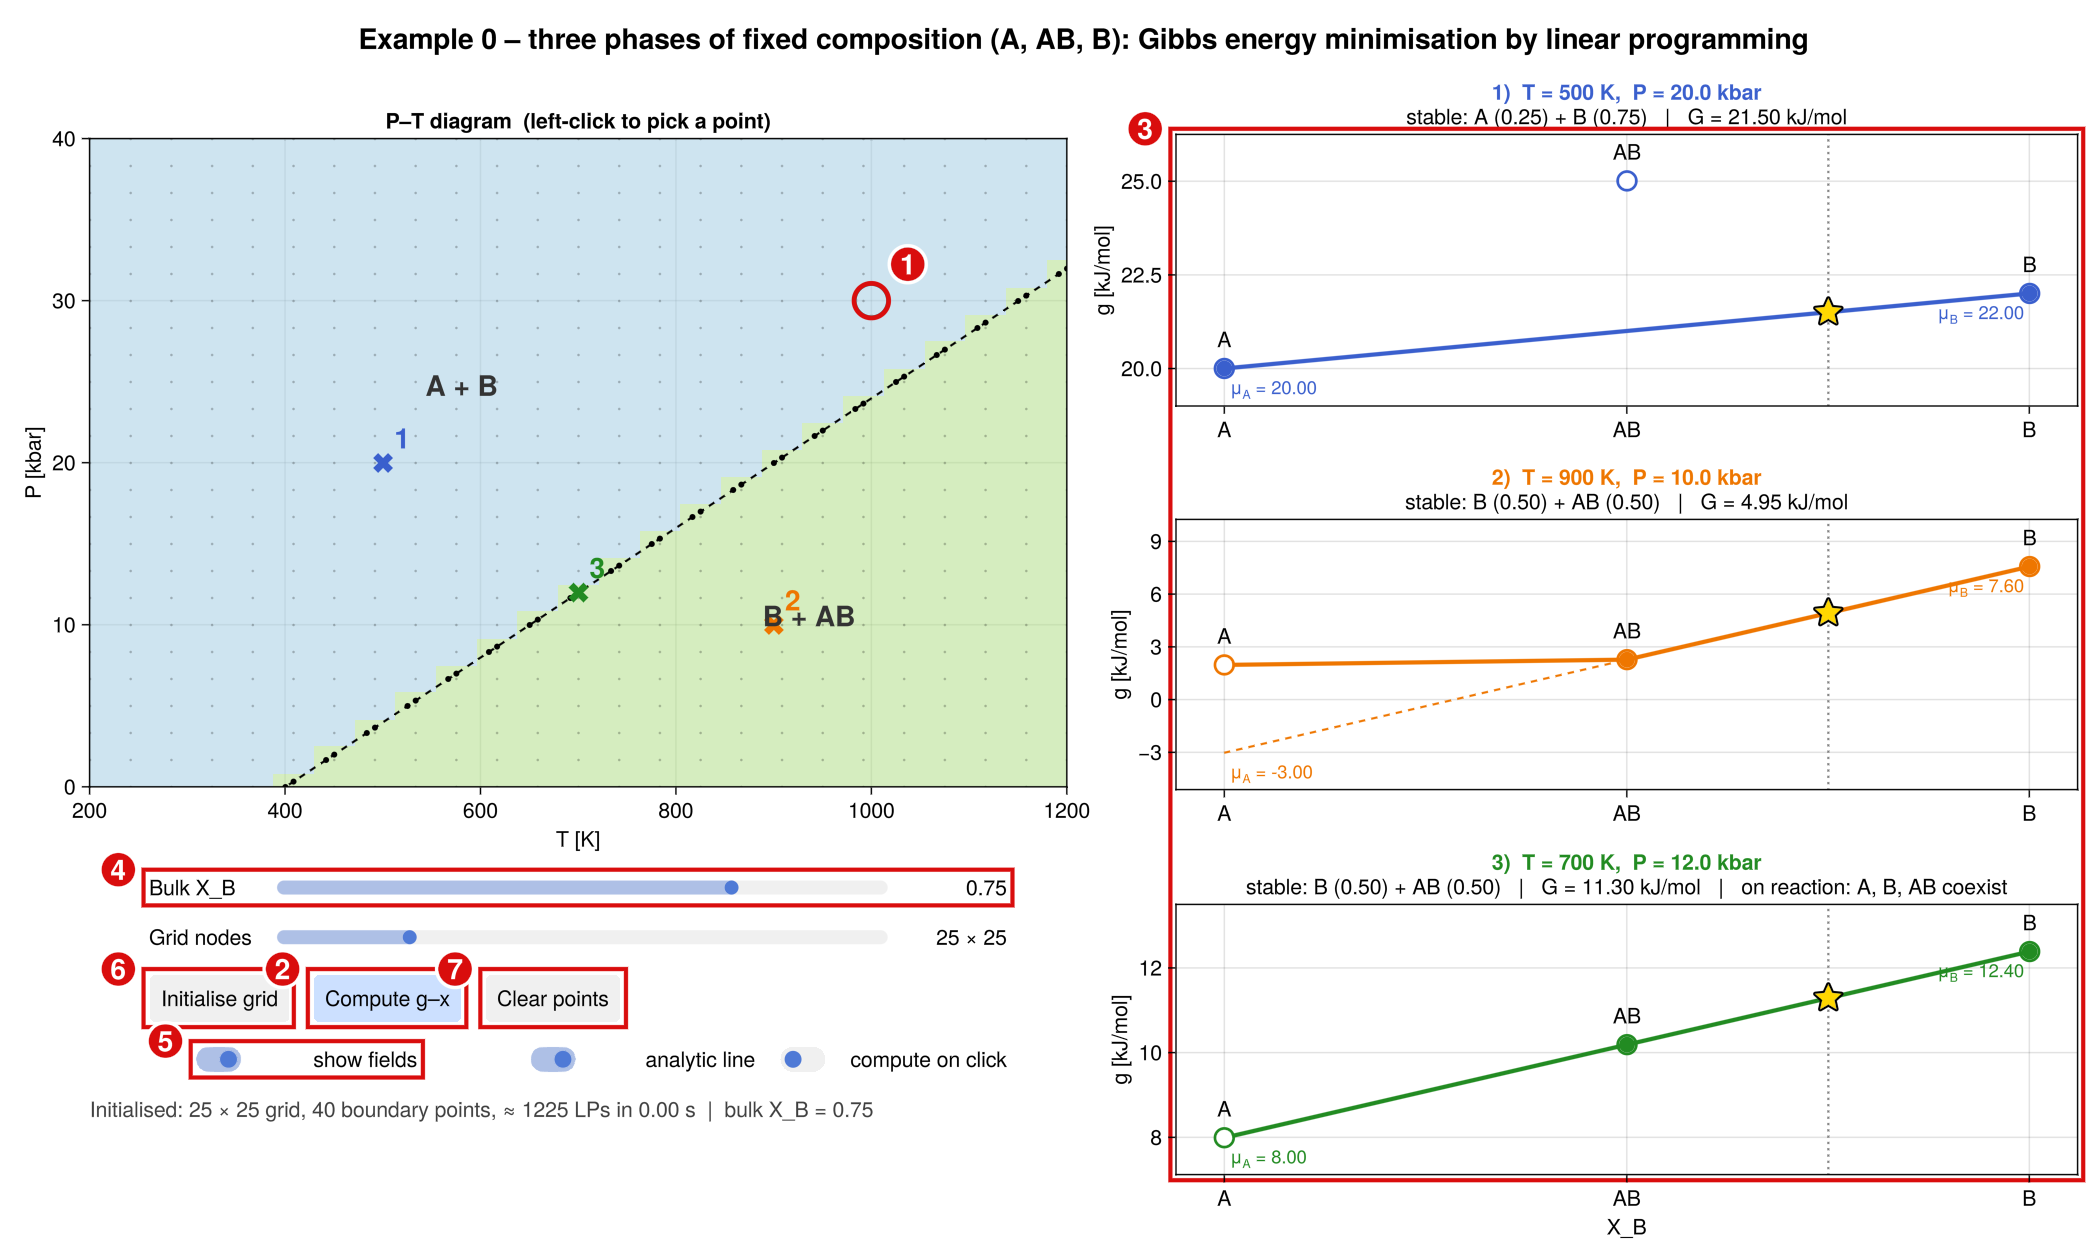
\includegraphics[width=0.85\textwidth]{figures/ex0_bulk075.png}
\caption{The same points with bulk $X_B = 0.75$: now AB + B instead of A + AB on the high-$T$ side.}
\end{figure}

\begin{tryit}
\begin{itemize}
\item Pick points on both sides of the line and exactly on it. When does AB touch the tangent of A and B?
\item Move \ctl{Bulk X\_B} through 0.5: why does the assemblage on the high-$T$ side change but not the position
  of the reaction line?
\item In the USER INPUT block, change the volume of AB. How does the slope of the line change (Clapeyron)?
\end{itemize}
\end{tryit}

%==============================================================================
\clearpage
\section{Example 1 – the solution playground (\texorpdfstring{$g$–$x$}{g–x})}\label{sec:ex1}
%==============================================================================
\textbf{File:} \file{Example1\_solution\_playground.jl}.\quad
\textbf{Phases} (each can be switched on and off): a solid solution $\alpha$ with a Margules parameter, the
pure phases A ($X_B=0$) and B ($X_B=1$), the compounds A2B ($X_B=\tfrac13$) and AB2 ($X_B=\tfrac23$) and an
ideal melt L. This example has no phase diagram; it shows one $g$–$x$ diagram that changes \emph{live} with
the sliders.

\begin{figure}[H]
\centering
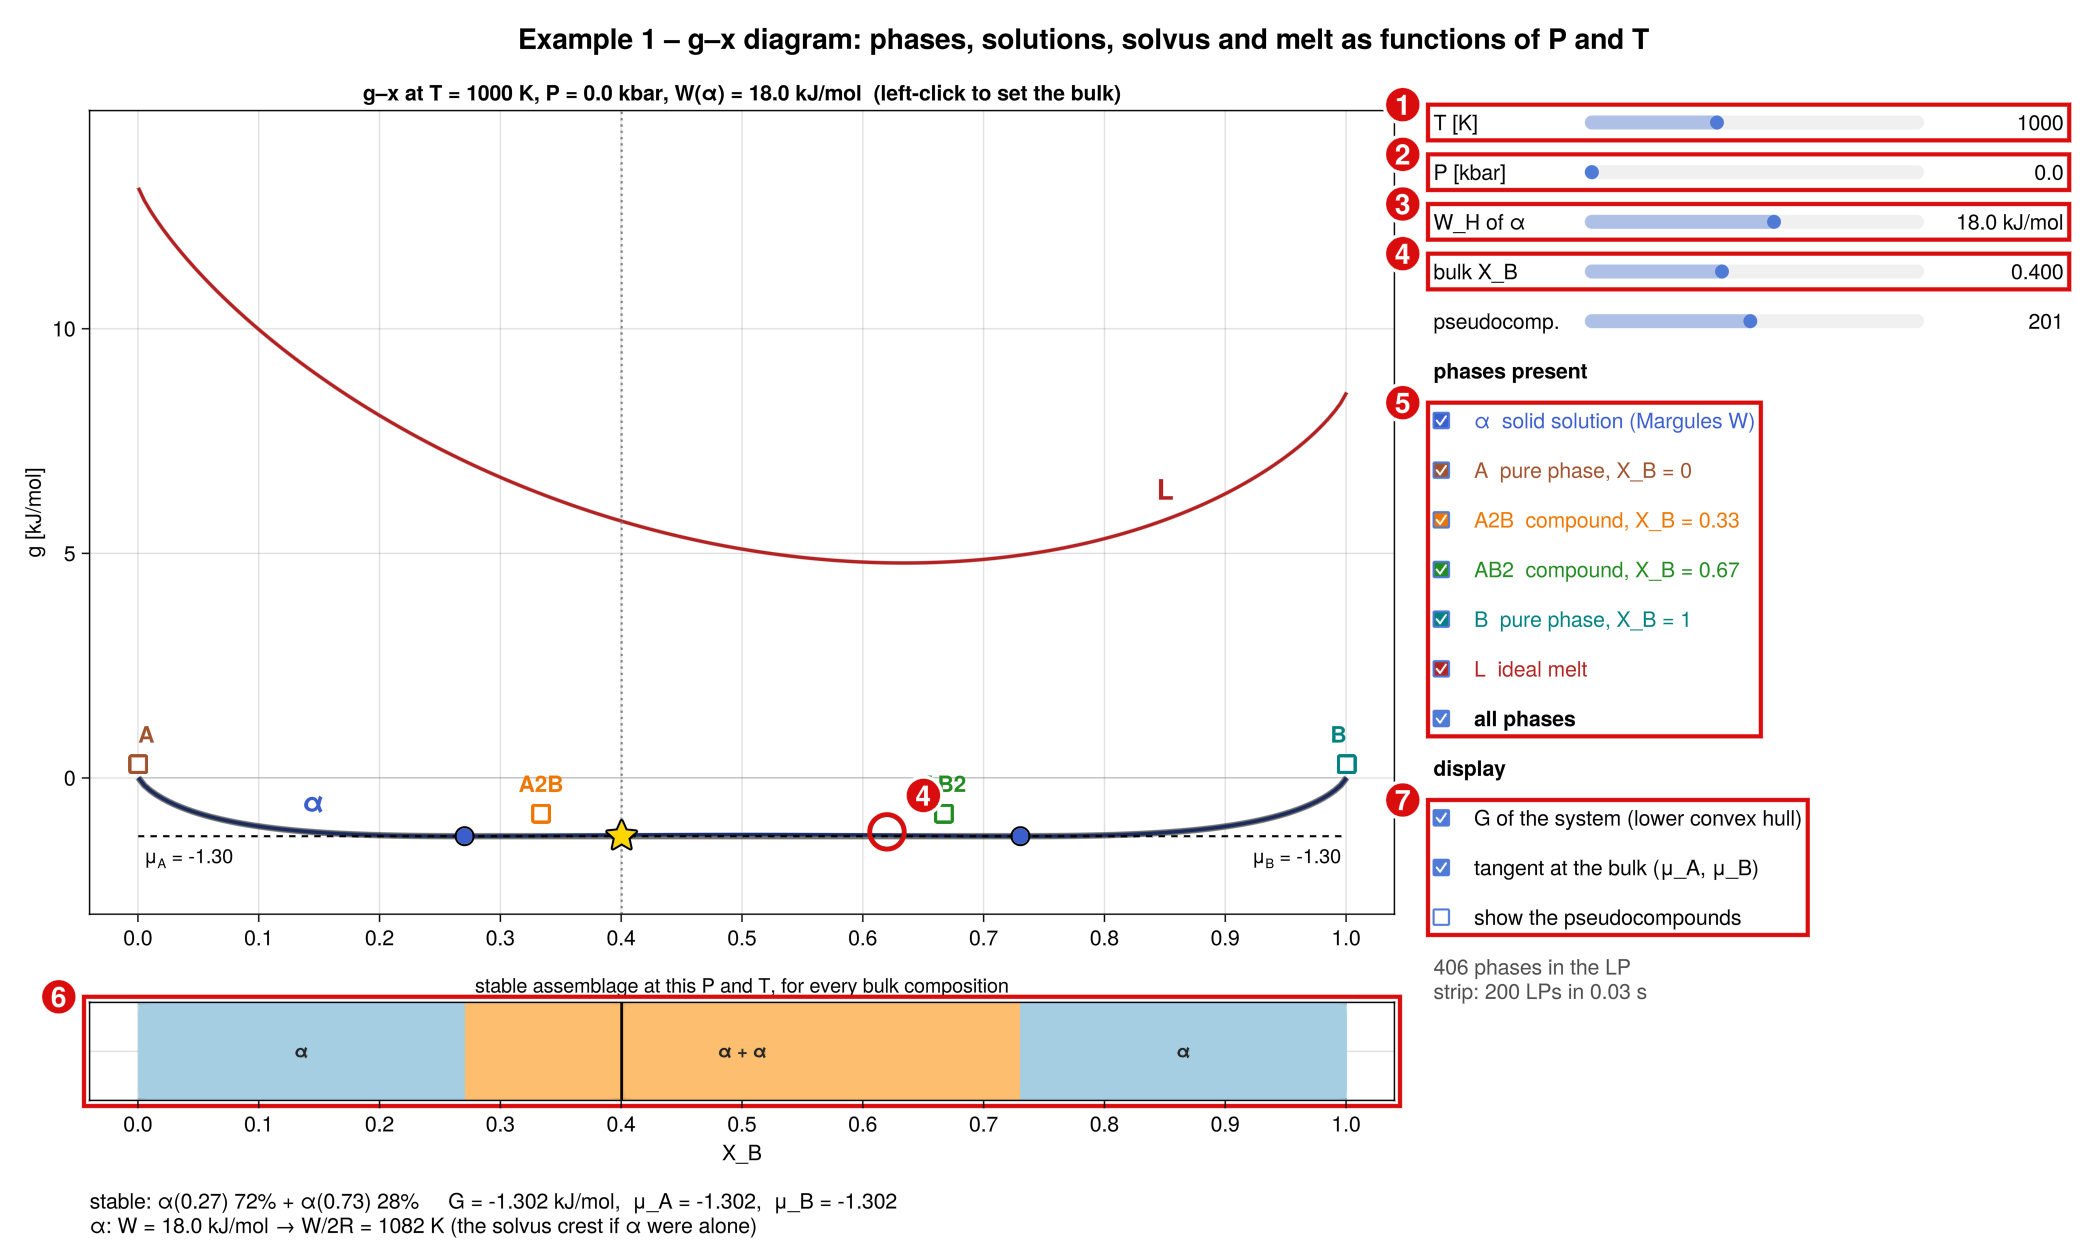
\includegraphics[width=\textwidth]{figures/ex1_overview.png}
\caption{Example 1 at 1000\,K: the $\alpha$ curve has a hump, the bulk composition lies in the solvus
($\alpha + \alpha$).}
\label{fig:ex1}
\end{figure}

\paragraph{Step by step} (numbers as in Fig.~\ref{fig:ex1})
\begin{enumerate}[label=\protect\step{\arabic*}]
\item \ctl{T [K]}: all curves and points move. Watch which phases form the lower hull.
\item \ctl{P [kbar]}: the same for pressure (the melt and the compounds have different volumes).
\item \ctl{W\_H of $\alpha$}: the Margules parameter of $\alpha$. The text at the bottom gives $W/(2R)$, the
  top of the solvus if $\alpha$ were alone.
\item \ctl{bulk X\_B}, or a \textbf{left click} in the $g$–$x$ diagram, sets the bulk composition (star). The
  stable phases are drawn as filled symbols on the tangent; their amounts are listed at the bottom.
\item Check boxes: switch every phase on or off, or all at once with \ctl{all phases}. A phase that is switched
  off is removed from the LP and from the plot. If the active phases cannot make the bulk composition, the
  program says so.
\item The strip shows the stable assemblage for \emph{every} bulk composition at this $P$ and $T$ (one LP per
  column): one horizontal line through a $T$–$X$ diagram.
\item Display options: the lower convex hull ($G$ of the system), the tangent and the individual
  pseudocompounds.
\end{enumerate}

\begin{figure}[H]
\centering
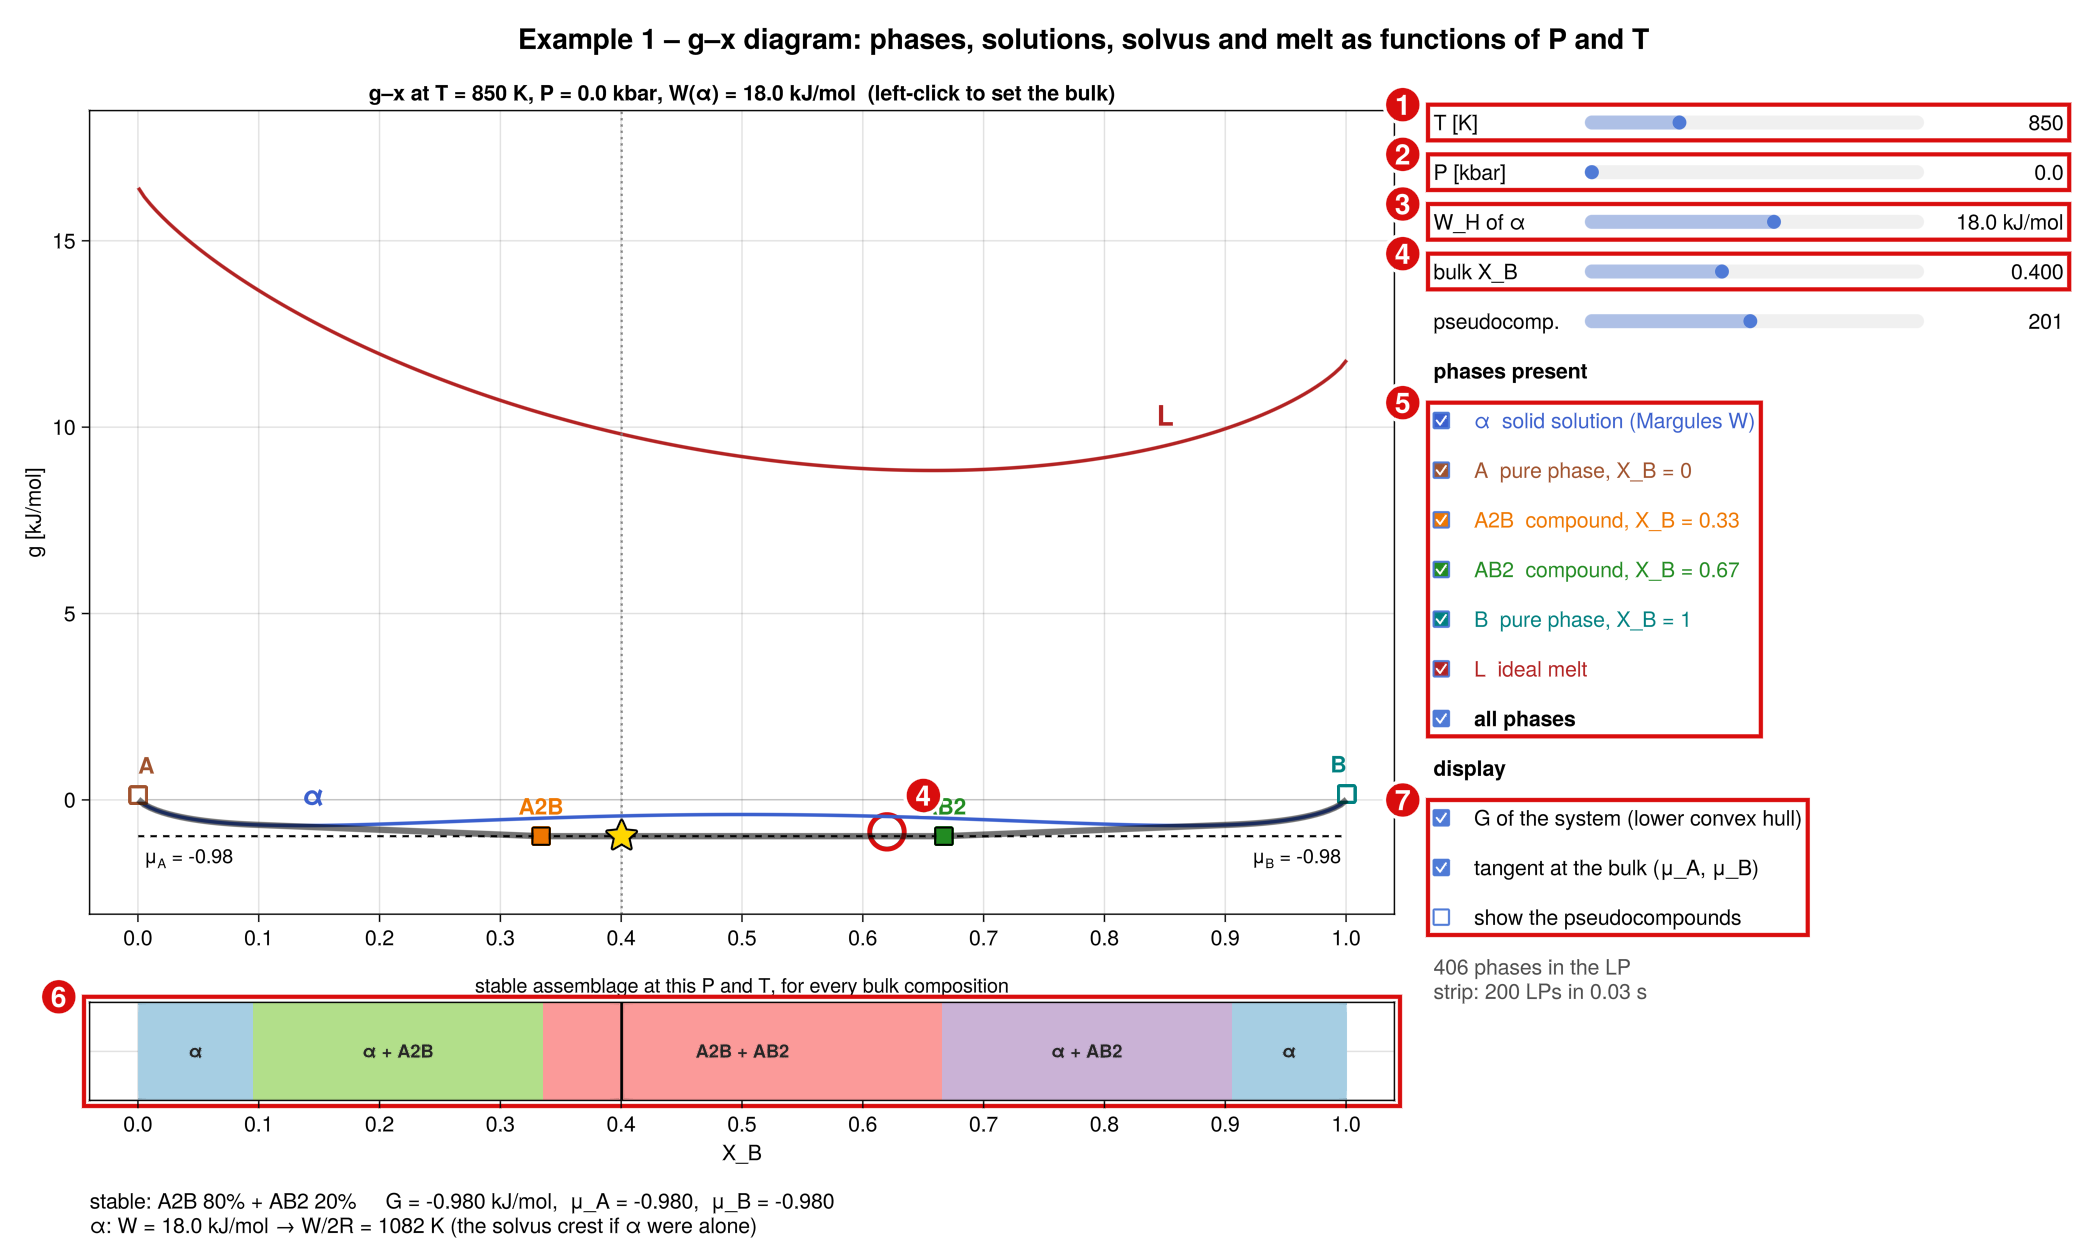
\includegraphics[width=0.49\textwidth]{figures/ex1_850K.png}\hfill
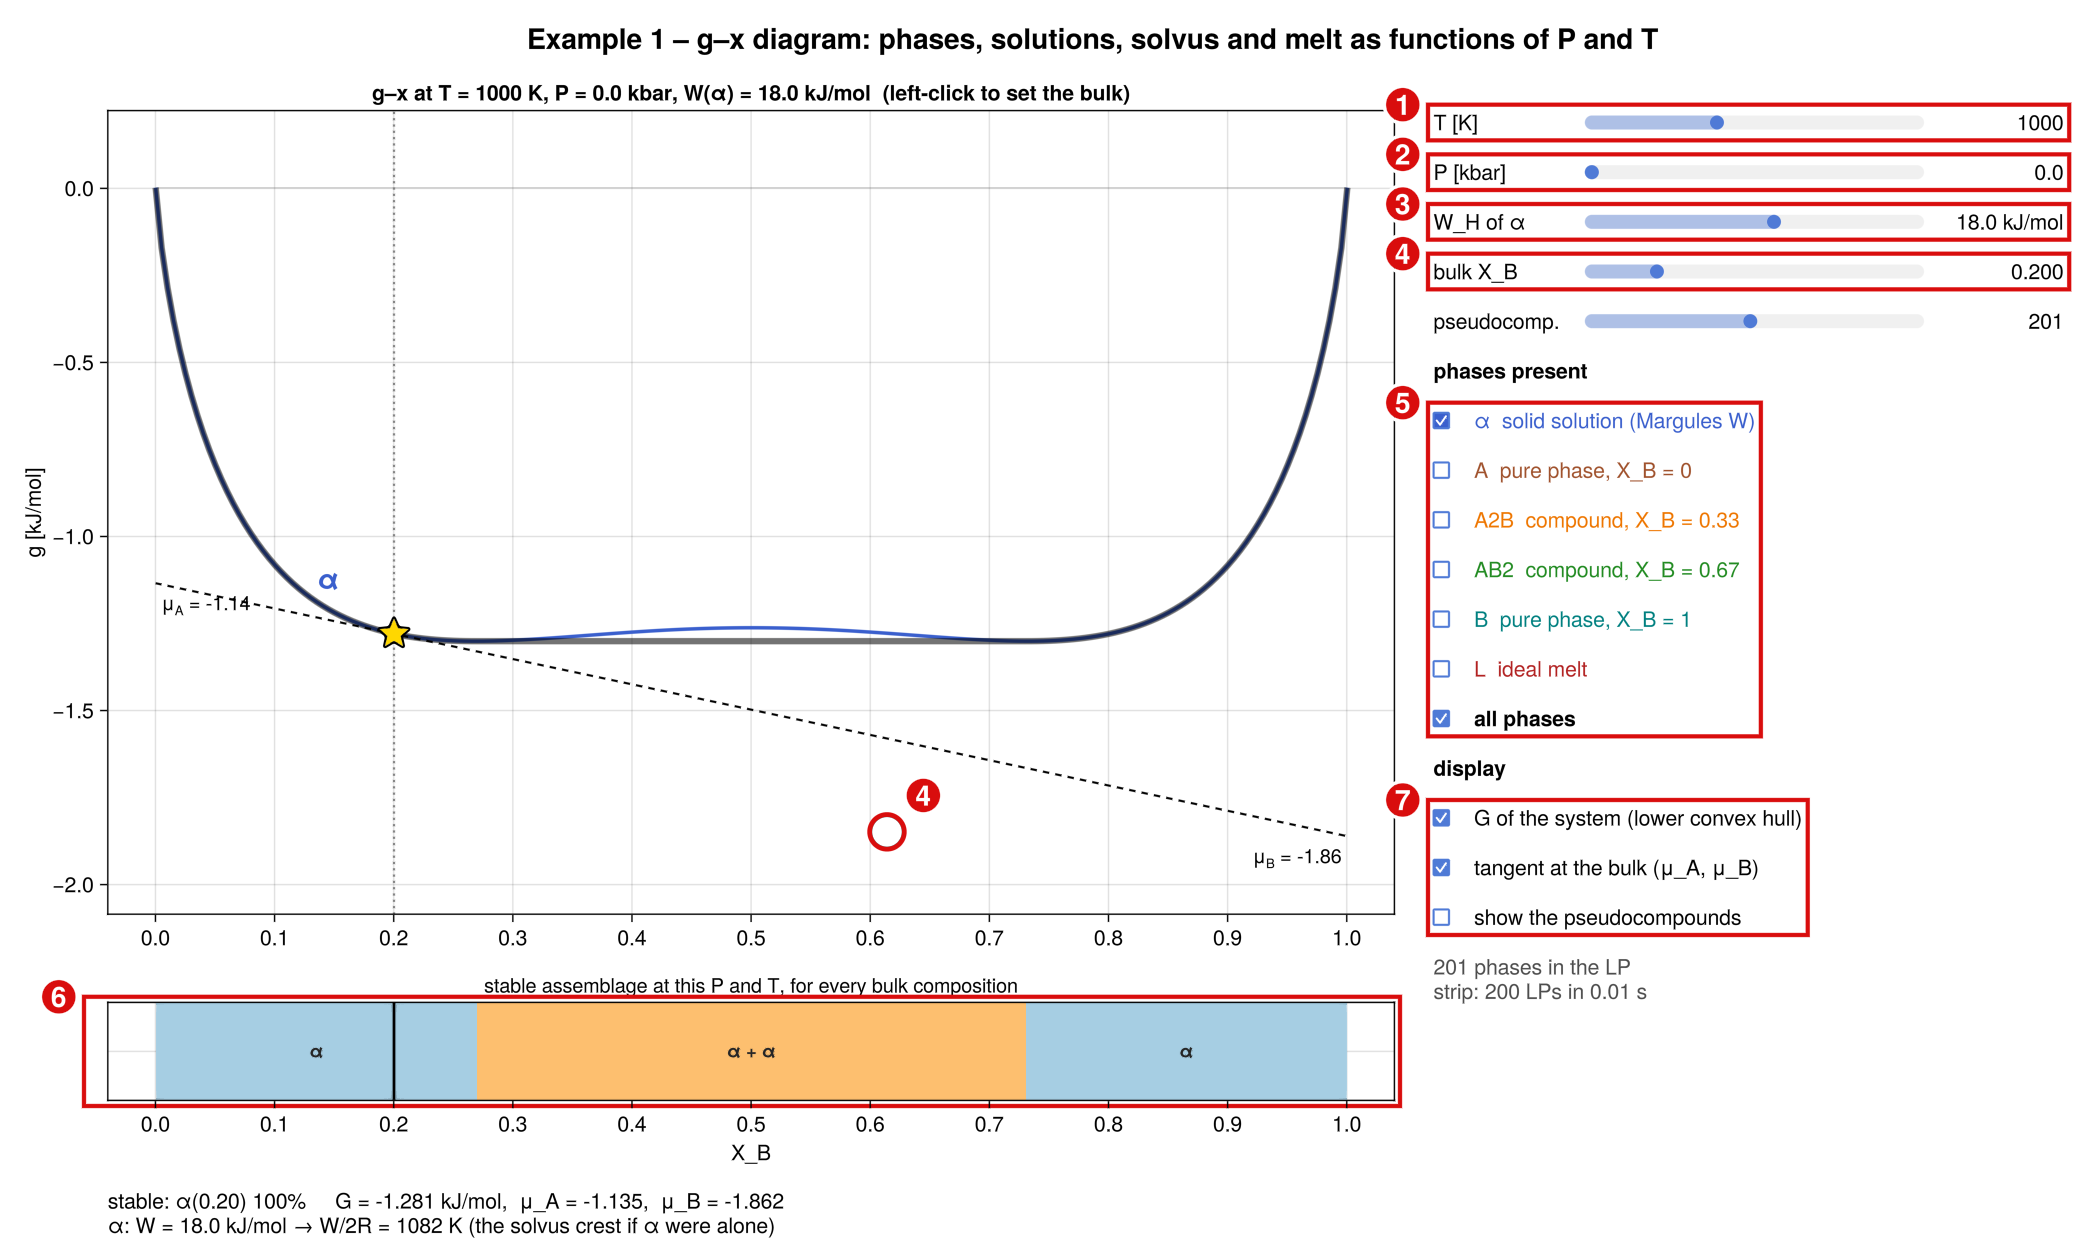
\includegraphics[width=0.49\textwidth]{figures/ex1_alpha_only.png}
\caption{Left: 850\,K, the compounds A2B and AB2 are stable. Right: only $\alpha$ switched on at 1000\,K: the
solvus and the common tangent of the two $\alpha$ compositions.}
\end{figure}

\begin{figure}[H]
\centering
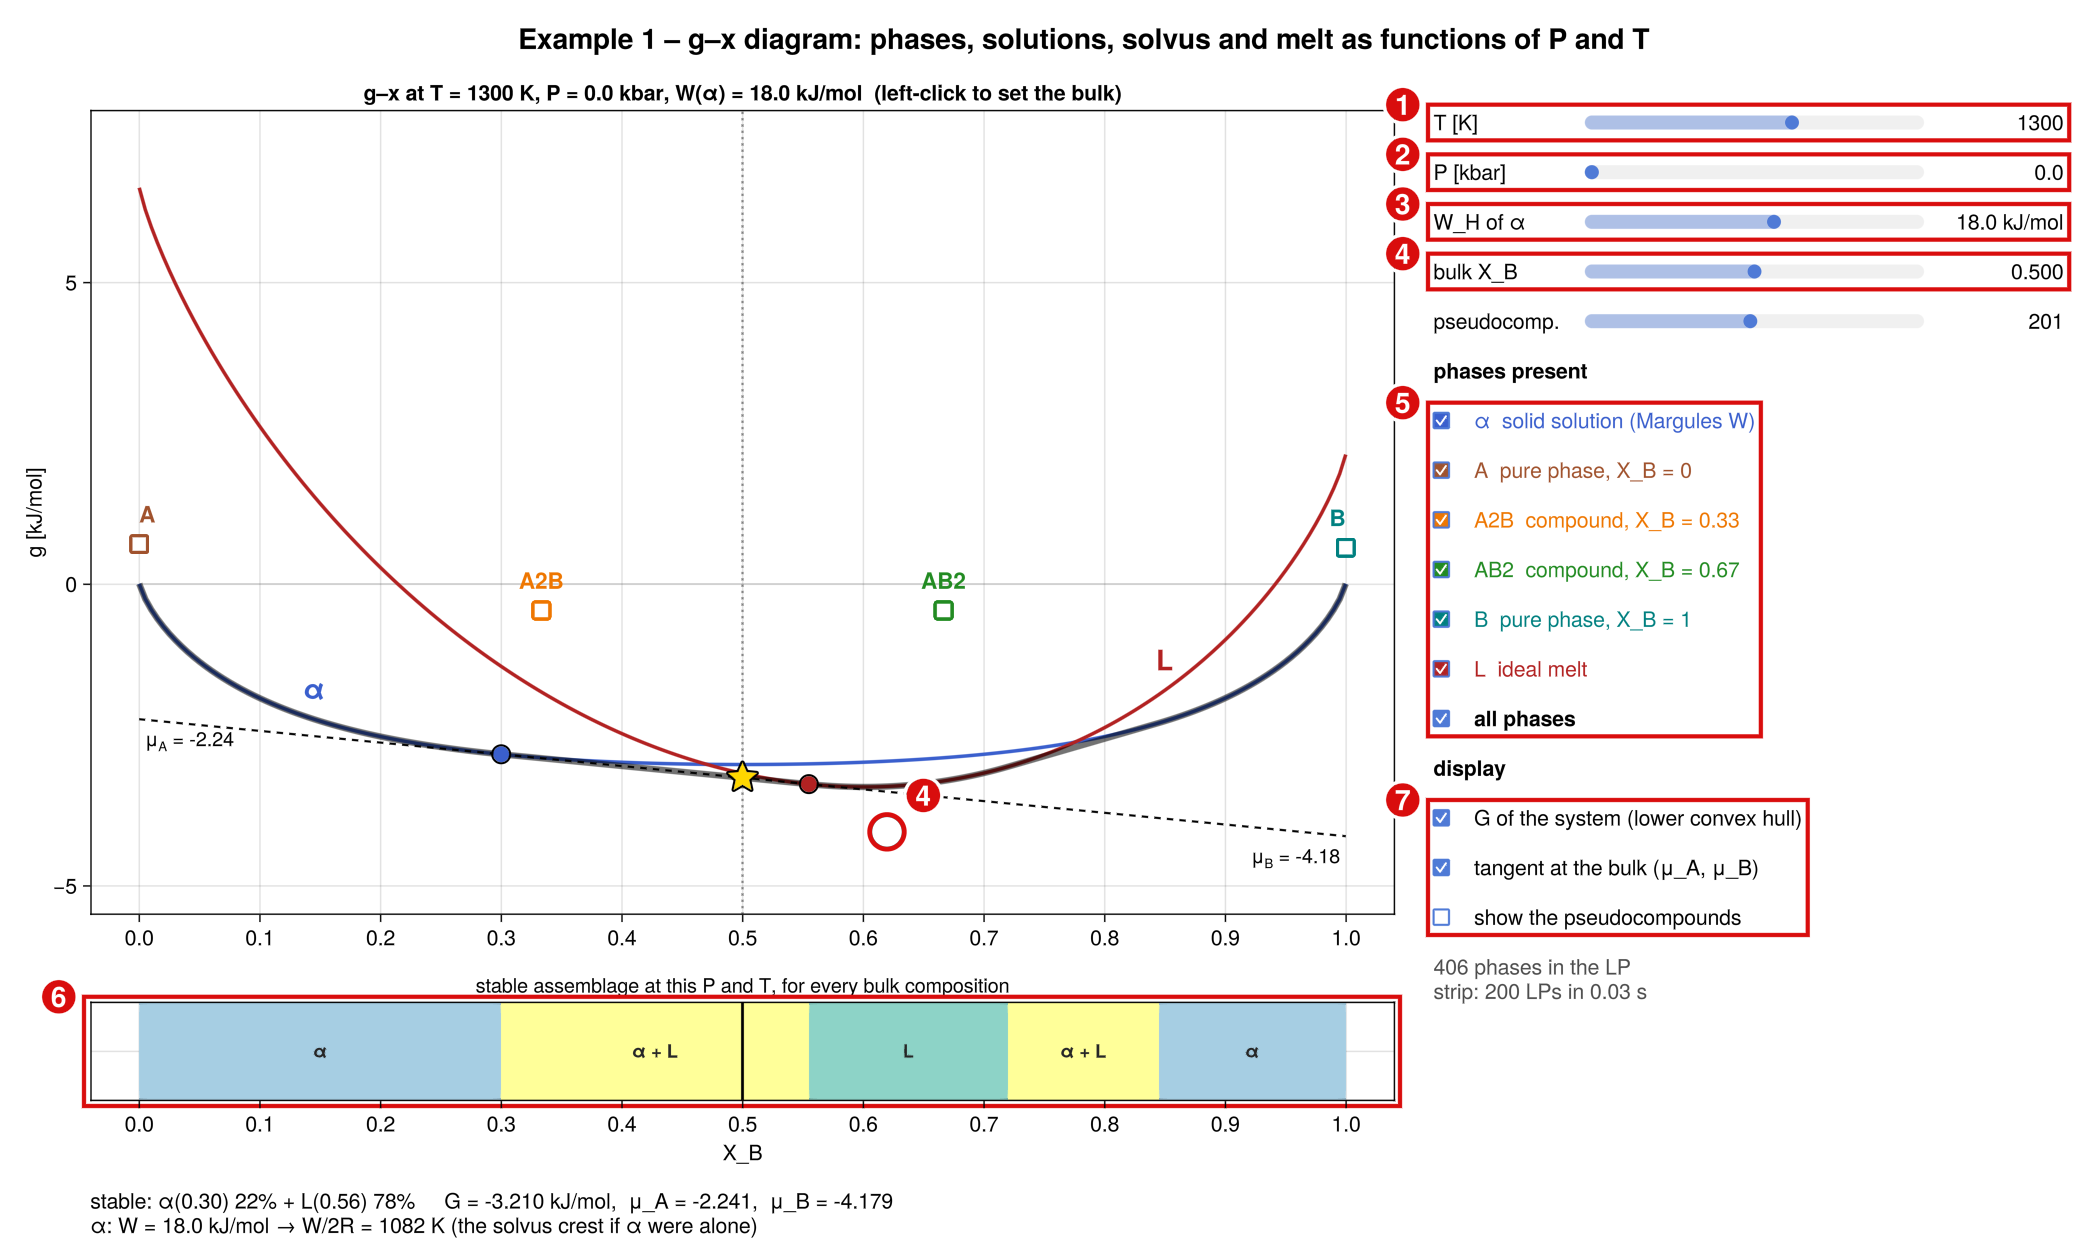
\includegraphics[width=0.6\textwidth]{figures/ex1_1300K.png}
\caption{1300\,K: the melt has come down; $\alpha$ + L, L, L + $\alpha$ across the composition range.}
\end{figure}

\paragraph{Default data at $P = 0$.} Pure A and B are stable below $\approx750$ and 700\,K (low-$T$ forms of the
$\alpha$ end-members); A2B and AB2 below $\approx 910$\,K; the $\alpha+\alpha$ solvus up to $\approx1085$\,K;
one $\alpha$ up to $\approx1285$\,K; then $\alpha$ + L and L.

\begin{tryit}
\begin{itemize}
\item Only $\alpha$ on: raise $W$ or lower $T$ until the solvus appears. Compare with $W/(2R)$.
\item $\alpha$ + compounds: at which $T$ do A2B and AB2 stop being stable?
\item Everything on: heat $X_B = 0.5$ from 800 to 1400\,K and name every assemblage; repeat at 15\,kbar.
\item $X_B = 0.05$, cool from 900\,K: where does pure A appear, and why at a lower $T$ than for $X_B = 0$?
\end{itemize}
\end{tryit}

%==============================================================================
\clearpage
\section{Example 2 – binary eutectic Di–An (\texorpdfstring{$T$–$X$}{T–X})}\label{sec:ex2}
%==============================================================================
\textbf{File:} \file{Example2\_eutectic\_TX.jl}.\quad
\textbf{Phases:} pure diopside (Di, CaMgSi$_2$O$_6$) and anorthite (An, CaAl$_2$Si$_2$O$_8$) and a melt L
(Eq.~\eqref{eq:sol}) whose end-members follow from the melting data (Eq.~\eqref{eq:melt}). The calculation
is in moles ($X$ = mole fraction of An); the diagram and the $g$–$x$ panels are shown in wt\% An
(Section~\ref{sec:weight}) and the temperature in $^\circ$C, as in the Di–An diagram of the course.

\paragraph{Calibration.} The melting points are those of the diagram (Di 1391\,$^\circ$C, An 1553\,$^\circ$C).
The two liquidus curves were read off the diagram (117 points in wt\%,
\file{data/\allowbreak DiAn\_liquidus\_digitized.txt}), converted to mole fractions, and $\Delta H$ of both end-members
and $W$ of the melt were fitted to them (\file{calibration/\allowbreak fit\_Example2\_DiAn.jl}):
$\Delta H_\mathrm{Di} = 128.1$\,kJ/mol, $\Delta H_\mathrm{An} = 154.7$\,kJ/mol, $W = -25.5$\,kJ/mol.
The model eutectic lies at 41.9\,wt\% An (35.9\,mol\%) and 1274\,$^\circ$C (diagram: 42\,wt\%,
1274\,$^\circ$C); the liquidus is reproduced within 2.2\,K (rms). These are fitted parameters of the model,
not calorimetric values.

\begin{figure}[H]
\centering
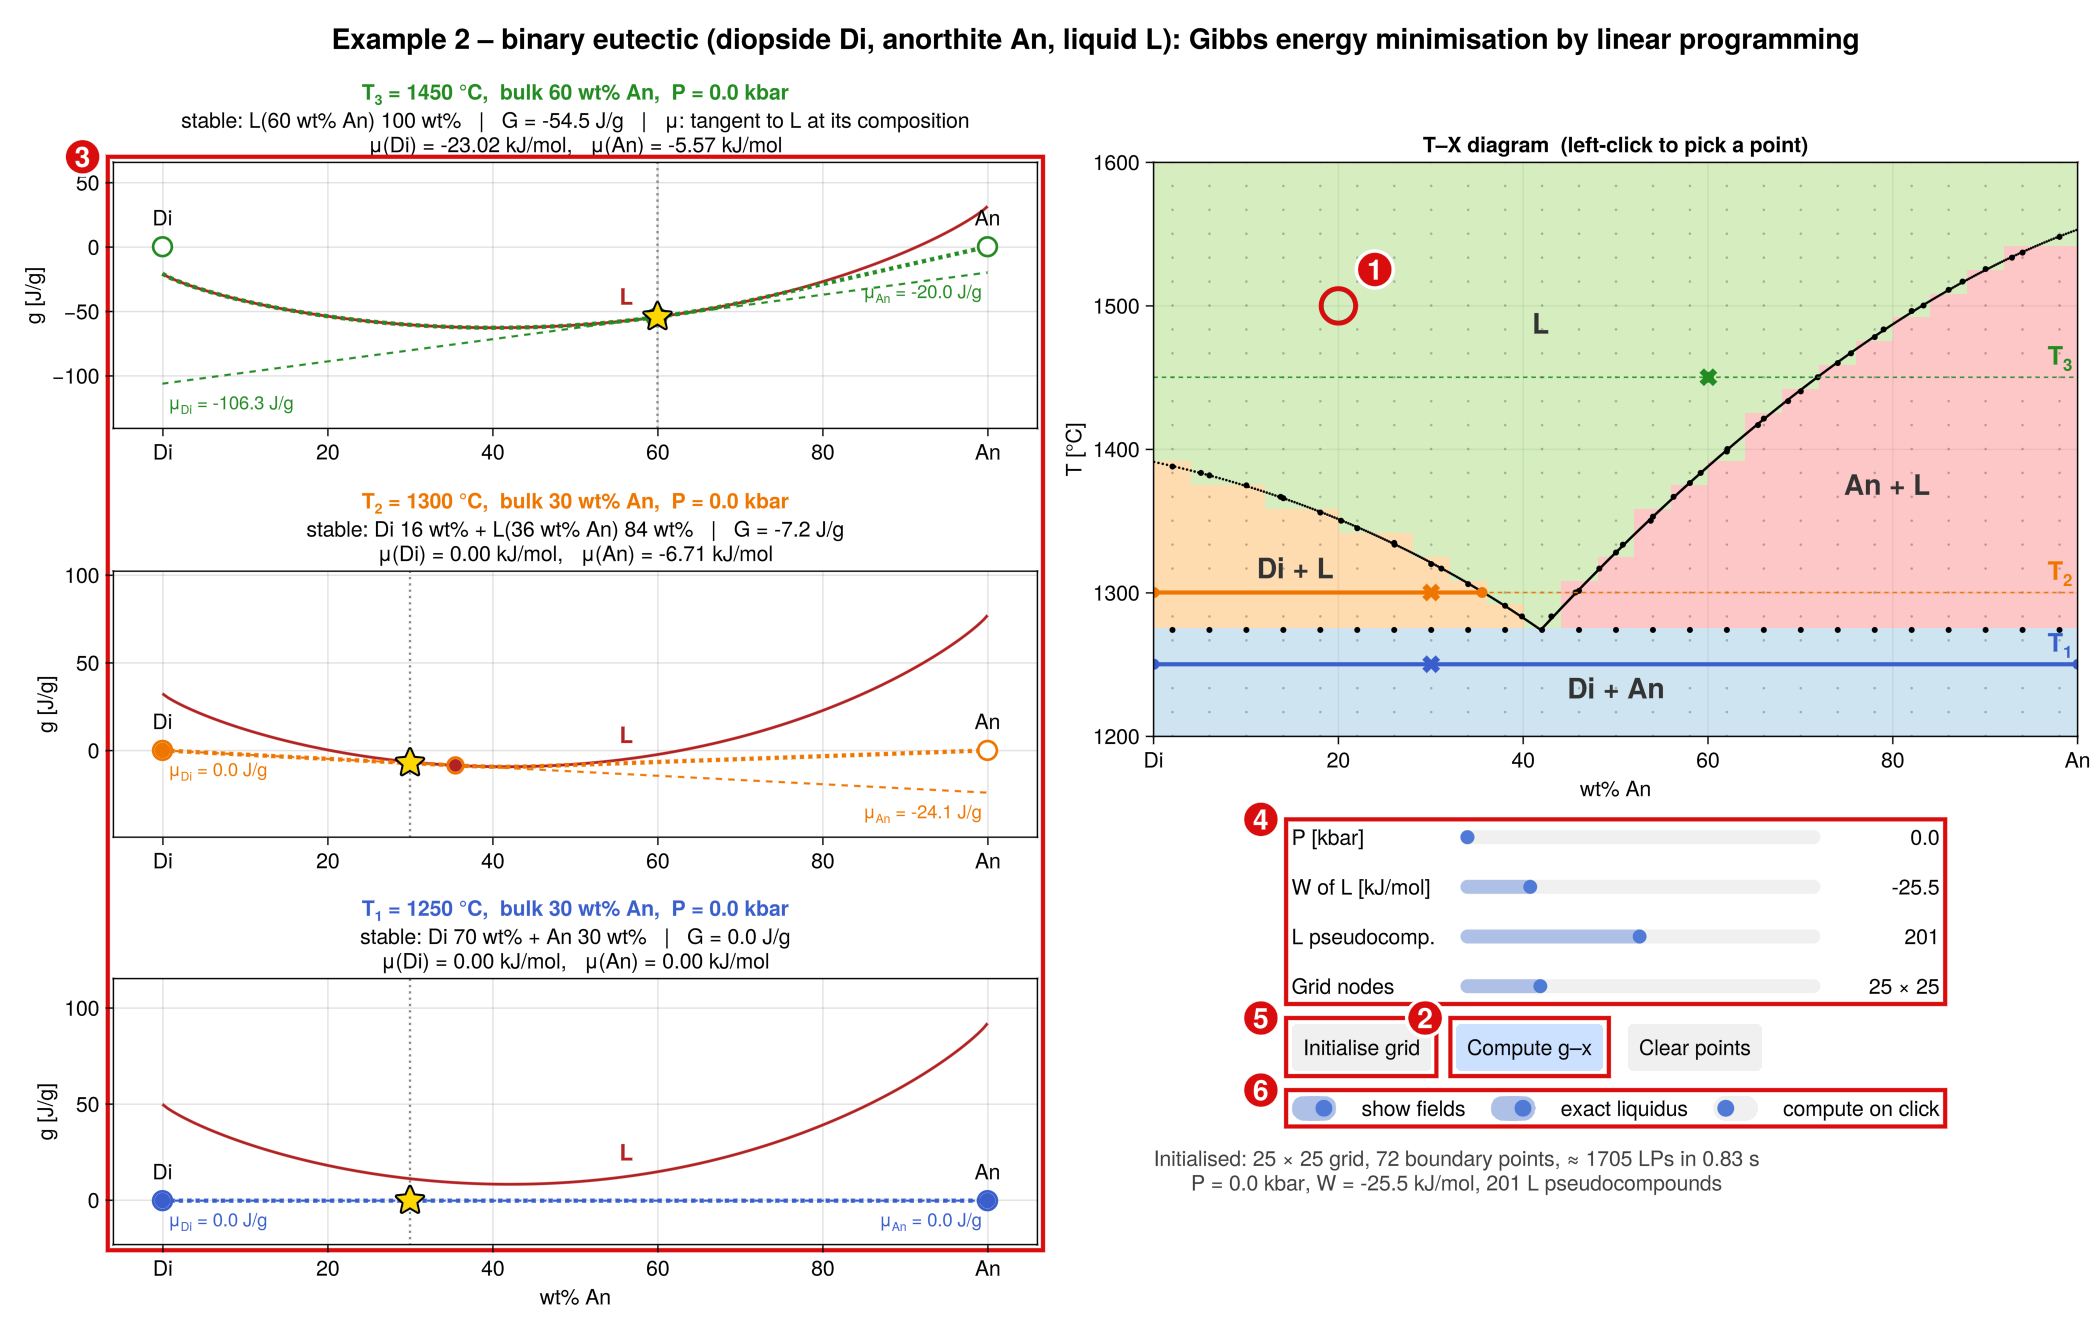
\includegraphics[width=\textwidth]{figures/ex2_overview.png}
\caption{Example 2 with three computed points at 30 and 60\,wt\% An: Di + An below the eutectic ($T_1$,
1250\,$^\circ$C), Di + L ($T_2$, 1300\,$^\circ$C) and melt only ($T_3$, 1450\,$^\circ$C).}
\label{fig:ex2}
\end{figure}

\paragraph{Step by step} (numbers as in Fig.~\ref{fig:ex2})
\begin{enumerate}[label=\protect\step{\arabic*}]
\item \textbf{Left-click} in the $T$–$X$ diagram: this picks a bulk composition \emph{and} a temperature.
\item Click \btn{Compute g–x}.
\item The $g$–$x$ diagrams appear on the left, \emph{sorted by temperature}: $T_1$ (lowest) at the bottom.
  The isotherm of every point and the tie-line between the coexisting phases are drawn in the $T$–$X$
  diagram. Red line: the melt; dotted: the lower hull; dashed: the tangent. $g$ is plotted per gram against
  wt\%, so the tangent is a straight line; its intercepts are $\mu_\mathrm{Di}$ and $\mu_\mathrm{An}$ per gram
  (the values in kJ/mol are given in brackets). The amounts of the phases are mass fractions.
\item Sliders: pressure, the Margules parameter $W$ of the melt, the number of pseudocompounds and the number
  of grid nodes. A new $P$ or $W$ recomputes the diagram automatically.
\item \btn{Initialise grid} recomputes the diagram (needed after changing \ctl{Grid nodes}).
\item \ctl{show fields}, \ctl{exact liquidus} (the liquidus computed without pseudocompounds, as a check of the
  LP) and \ctl{compute on click}. \btn{Clear points} empties the panels.
\end{enumerate}

\begin{tryit}
\begin{itemize}
\item Follow a melt with 30\,wt\% An on cooling: where does Di start to crystallise, how does the melt
  composition change, what happens at the eutectic? Repeat with 60\,wt\% An.
\item Use the lever rule: how much Di has crystallised from the 30\,wt\% An melt at 1300\,$^\circ$C? Compare with
  the amounts (in wt\%) printed above the $g$–$x$ panel.
\item The eutectic melt has 42\,wt\% An. Convert this to mol\% with Eq.~\eqref{eq:wt} (answer: 36\,mol\%).
  Which of the two numbers belongs into Eq.~\eqref{eq:sol}?
\item Set \ctl{W of L} to 0 (ideal melt): how much do the eutectic and the liquidus move? Then raise it above
  about +30\,kJ/mol: the melt unmixes (L + L).
\item Reduce the pseudocompounds to 11: why does the liquidus become a staircase?
\end{itemize}
\end{tryit}

%==============================================================================
\clearpage
\section{Example 3 – binary peritectic Fo–SiO\texorpdfstring{$_2$}{2}}\label{sec:ex3}
%==============================================================================
\textbf{File:} \file{Example3\_peritectic\_TX.jl}.\quad
Same program as Example 2 for the system forsterite (Fo, Mg$_2$SiO$_4$) – silica (cristobalite, Crs), with
enstatite (En, MgSiO$_3$ = $\tfrac12$Mg$_2$SiO$_4$ + $\tfrac12$SiO$_2$; protoenstatite, ``Pr'' in the diagram)
as an intermediate solid that melts \emph{incongruently}: at the peritectic it breaks down to Fo plus a melt
that is richer in SiO$_2$ than En. Silica-rich melts unmix into two liquids (L + L) above about
1695\,$^\circ$C. The calculation is in moles ($X$ = mole fraction of SiO$_2$ between Mg$_2$SiO$_4$ and
SiO$_2$; En lies at $X = 0.5$). The diagram is shown in wt\% SiO$_2$ of the whole system, as the Fo–SiO$_2$
diagram of the course (Morse 1980, Fig.~10.1, after Bowen and Andersen): forsterite lies at 42.7\,wt\%,
enstatite at 59.85\,wt\% and silica at 100\,wt\% SiO$_2$ (Section~\ref{sec:weight}). The temperature is in
$^\circ$C. The controls are the same as in Example~2 (Fig.~\ref{fig:ex2}); the slider \ctl{$\Delta$W of L}
adds a regular-solution term $\Delta W\,X(1-X)$ to the calibrated melt, and \ctl{exact boundaries} shows
the liquidus and the two-liquid field of the continuous melt (no pseudocompounds).

\paragraph{Calibration.} {\sloppy The curves of the diagram were read off in wt\% SiO$_2$ (229 points,
\file{data/\allowbreak FoSiO2\_liquidus\_\allowbreak Morse\_digitized.txt}), converted to mole fractions and fitted
(\file{calibration/\allowbreak fit\_Example3\_FoSiO2.jl}). The melting points are those of the diagram (Fo
1890\,$^\circ$C, Crs 1713\,$^\circ$C) and $\Delta H_\mathrm{Fo} = 142$\,kJ/mol is the value used in
Example~4. Fitted were $\Delta H_\mathrm{SiO_2} = 18.19$\,kJ/mol, the Gibbs energy of En ($-2.414$\,kJ/mol
relative to $\tfrac12$Fo + $\tfrac12$SiO$_2$) and the excess terms of the melt, Eq.~\eqref{eq:rk}, with
$a = (129.53,\ 28.01,\ 111.27)$\,kJ/mol and $b = (0.07848,\ 0.02667,\ 0.03521)$\,kJ/(mol\,K).\par}
\begin{center}\small
\begin{tabular}{@{}lllll@{}}
\toprule
 & \multicolumn{2}{l}{model} & \multicolumn{2}{l}{diagram} \\
 & $T$ [$^\circ$C] & melt [wt\% SiO$_2$] & $T$ [$^\circ$C] & melt [wt\% SiO$_2$] \\ \midrule
peritectic (En $\to$ Fo + L) & 1555.5 & 61.3 & 1557 & $\approx$61.3 \\
eutectic (En + Crs + L) & 1545.3 & 64.8 & 1543 & $\approx$65.0 \\
two liquids + Crs & 1697.8 & 69.3 and 98.7 & 1695 & $\approx$69.4 and 98.7 \\
\bottomrule
\end{tabular}
\end{center}
The liquidus is reproduced within 3.9\,K (rms, 134 points) and the two-liquid field within 0.7\,wt\%
SiO$_2$ (rms). Three excess terms are needed because the melt mixes with a negative excess energy next to
forsterite and unmixes next to silica. These are fitted parameters of the model, not calorimetric values
(except $\Delta H_\mathrm{Fo}$); the pressure dependence is illustrative.

\begin{figure}[H]
\centering
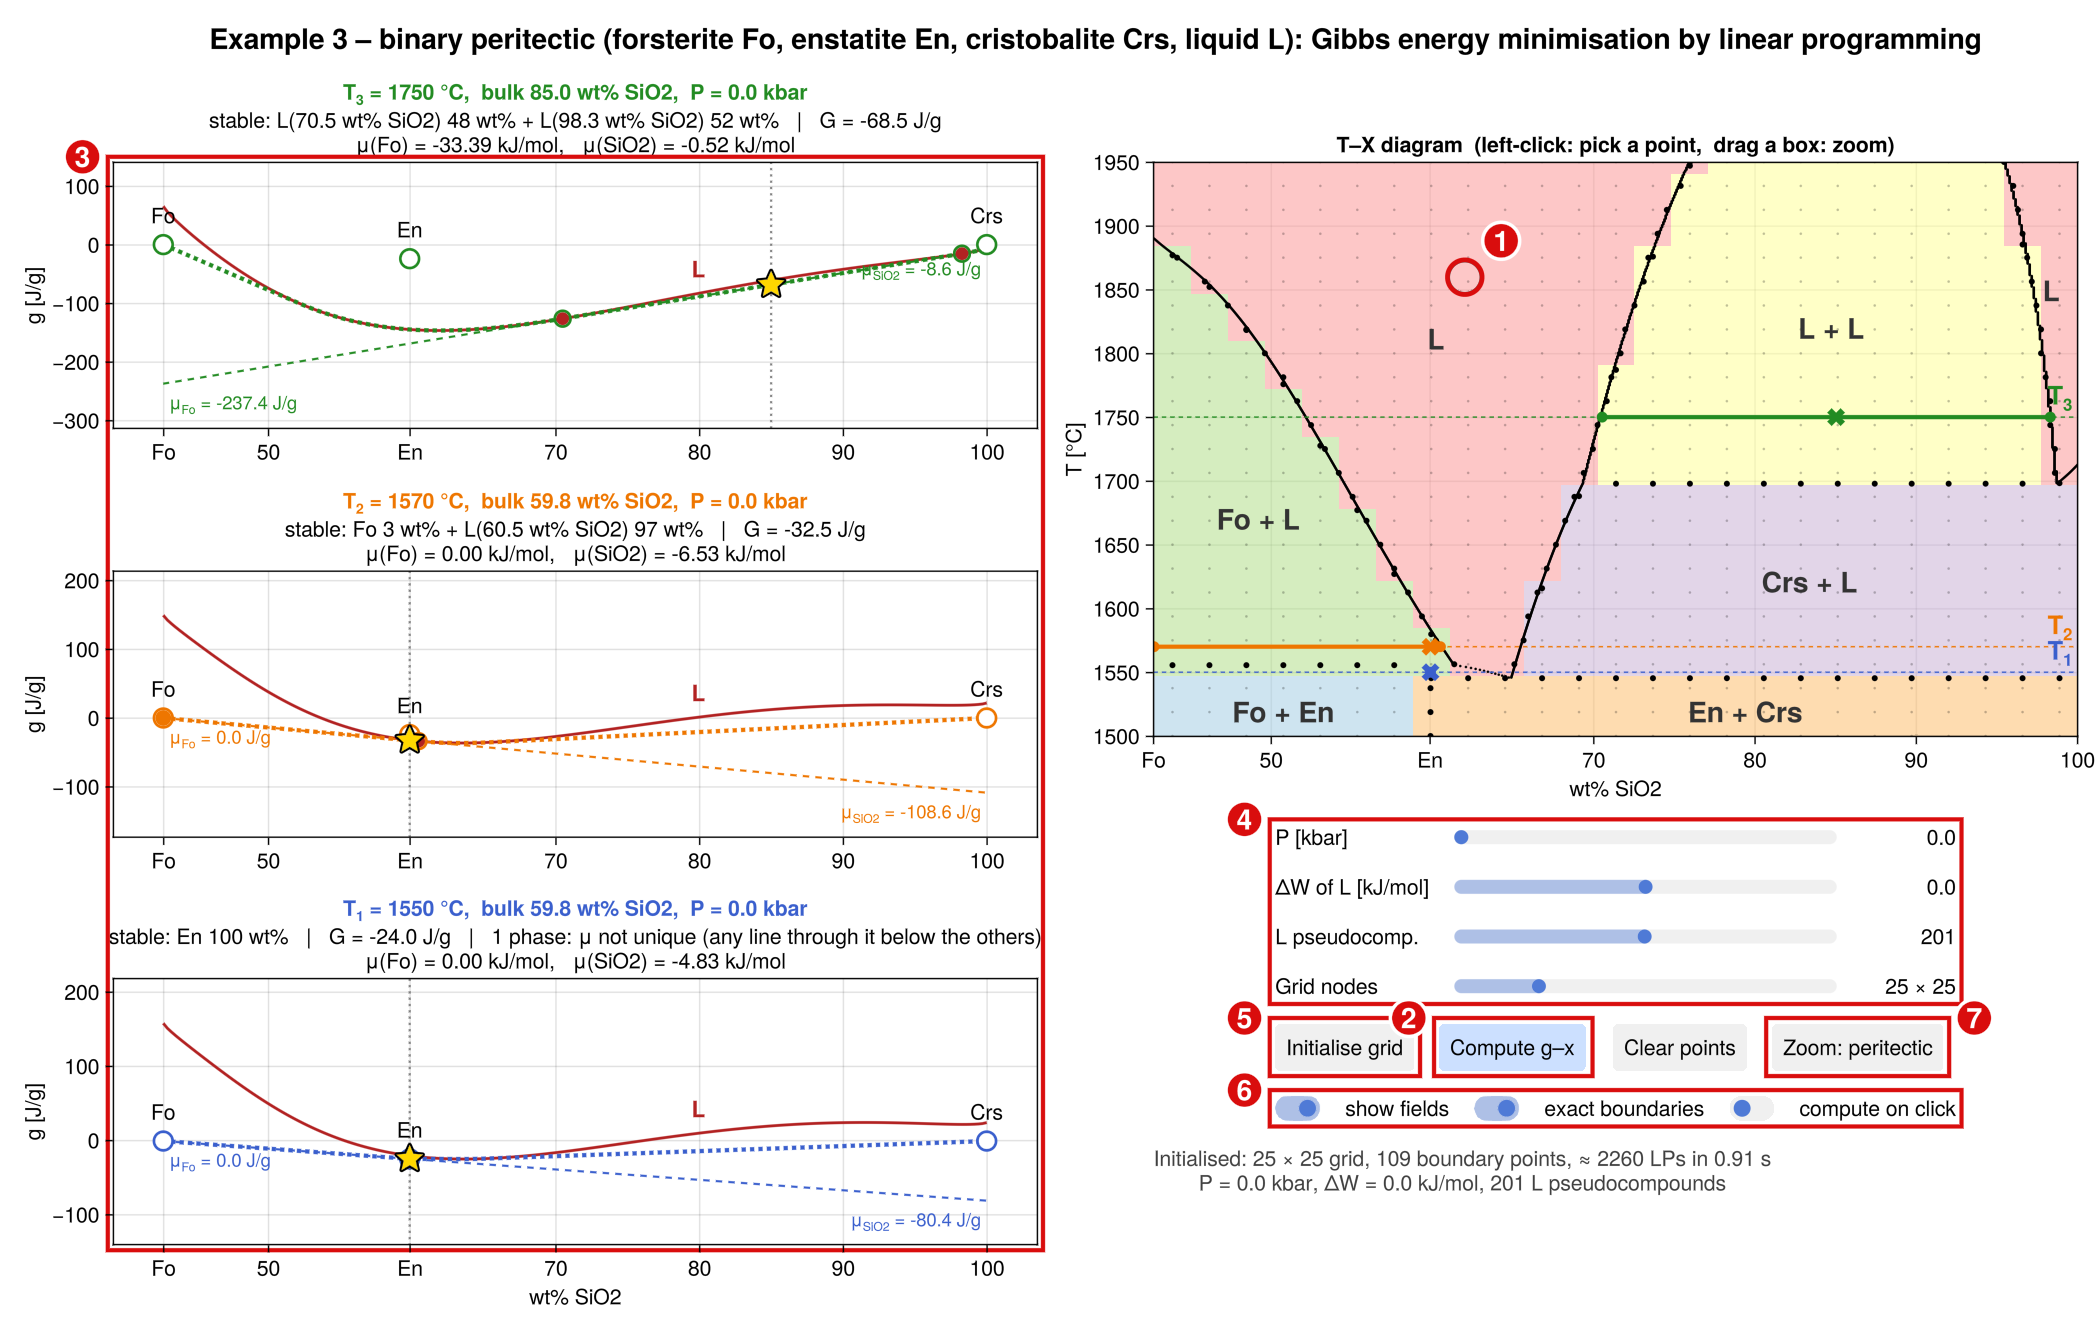
\includegraphics[width=\textwidth]{figures/ex3_overview.png}
\caption{Example 3: at the En composition (59.85\,wt\% SiO$_2$), En alone at 1550\,$^\circ$C ($T_1$) and
Fo + L at 1570\,$^\circ$C ($T_2$, above the peritectic: En lies above the tangent from Fo to the melt); two
liquids at 85\,wt\% SiO$_2$ and 1750\,$^\circ$C ($T_3$: the melt curve has a hump). The numbers
\protect\step{1}–\protect\step{6} are those of Fig.~\ref{fig:ex2}; \protect\step{7} is the zoom.}
\label{fig:ex3}
\end{figure}

\paragraph{Zoom} (\step{7} in Fig.~\ref{fig:ex3}). The En + L field is only 10\,$^\circ$C high: with
$25 \times 25$ grid nodes it falls between the nodes of the whole diagram and is not drawn. The $T$–$X$
diagram can therefore be zoomed:
\begin{itemize}
\item \btn{Zoom: peritectic} shows a window around En and the peritectic temperature
  (Fig.~\ref{fig:ex3zoom}). The temperature is found with the LP at the current pressure and $\Delta W$, so
  the window follows the peritectic when you move the sliders.
\item \textbf{Drag a box} with the left mouse button to zoom on any other part of the diagram. A click
  without moving the mouse still picks a point.
\item While a part of the diagram is shown, the same button reads \btn{Zoom: full diagram} and goes back.
\end{itemize}
The grid, its boundary points and the exact boundaries are computed again inside the window; \btn{Initialise
grid} and the sliders also act on the window that is shown. The liquid pseudocompounds stay the same, so in a
small window their spacing shows as steps in the fields. The $g$–$x$ panels are not changed by this zoom:
they show the whole composition range.

\begin{figure}[H]
\centering
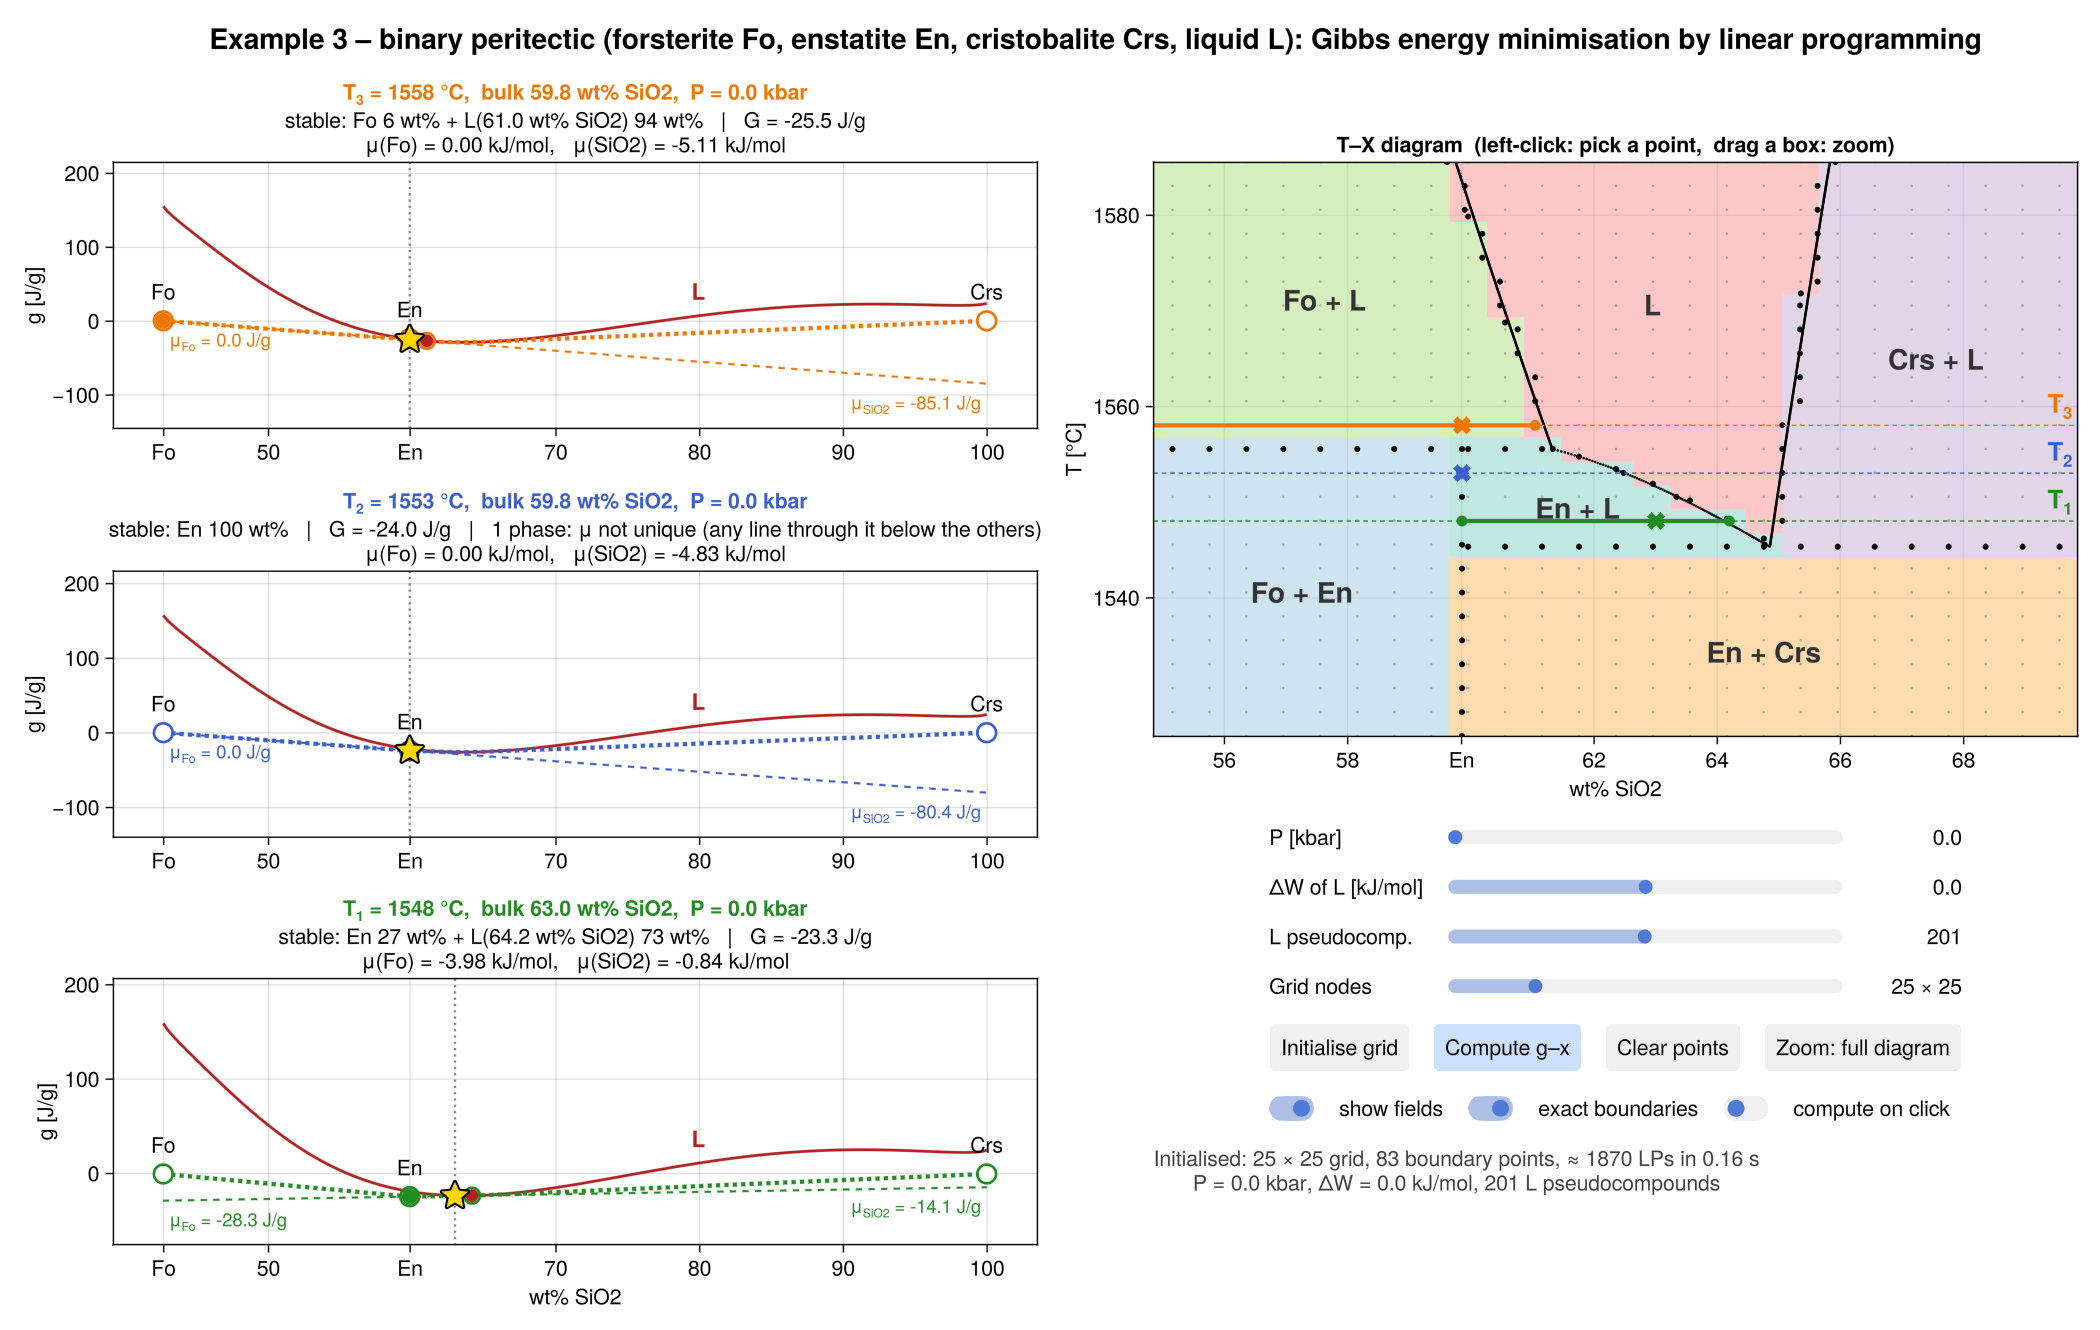
\includegraphics[width=0.85\textwidth]{figures/ex3_peritectic.png}
\caption{Example 3 after \btn{Zoom: peritectic}: the En + L field between the peritectic
(1555.5\,$^\circ$C) and the eutectic (1545.3\,$^\circ$C) is resolved. At the En composition: En alone at
1553\,$^\circ$C ($T_2$) and Fo + L at 1558\,$^\circ$C ($T_3$). En + L at 63\,wt\% SiO$_2$ and
1548\,$^\circ$C ($T_1$).}
\label{fig:ex3zoom}
\end{figure}

\begin{tryit}
\begin{itemize}
\item Click \btn{Zoom: peritectic}. Pick points at the En composition just below and just above
  1556\,$^\circ$C and compare the position of En relative to the tangent. Then switch on \ctl{compute on
  click} and follow a melt with 63\,wt\% SiO$_2$ from 1565 to 1540\,$^\circ$C.
\item Cool melts with 55, 60.5, 63 and 67\,wt\% SiO$_2$: which phases appear and disappear, and what is the
  last melt? Why does the melt with 60.5\,wt\% first crystallise forsterite and end without it?
\item Pick 85\,wt\% SiO$_2$ at 1750\,$^\circ$C: two liquids. Where is the hump of the melt curve? Move
  \ctl{$\Delta$W of L} to $-20$ and to $+10$\,kJ/mol: how does the two-liquid field change?
\item Enstatite has 59.85\,wt\% SiO$_2$. Show with Eq.~\eqref{eq:wt} that this is $X = 0.5$ between
  Mg$_2$SiO$_4$ and SiO$_2$.
\item Increase the pressure: how do the peritectic and the eutectic move? In the USER INPUT block give En a
  volume of $-0.1$\,kJ/kbar (it is then favoured by pressure) and go to 30\,kbar: does En still melt
  incongruently?
\end{itemize}
\end{tryit}

%==============================================================================
\clearpage
\section{Example 4 – melting of a solid solution: olivine}\label{sec:ex4}
%==============================================================================
\textbf{File:} \file{Example4\_olivine\_loop\_TX.jl}.\quad
\textbf{Phases:} olivine Ol (solid solution of forsterite Fo and fayalite Fa) and a melt L; both are
solutions of the type \eqref{eq:sol} with $n = 2$ mixing sites. The calculation is in moles
($X_\mathrm{Fa}$ = mole fraction of fayalite); the diagram and the $g$–$x$ panels are shown in wt\% Fa
(Section~\ref{sec:weight}), the temperature is in $^\circ$C. Melting data: Fo 1890\,$^\circ$C, $\Delta H = 142$\,kJ/mol;
Fa 1205\,$^\circ$C, $\Delta H = 89.3$\,kJ/mol. With $W = 0$ the result is the classic melting \emph{loop}; its
closed-form solution is drawn as dashed lines.

\begin{figure}[H]
\centering
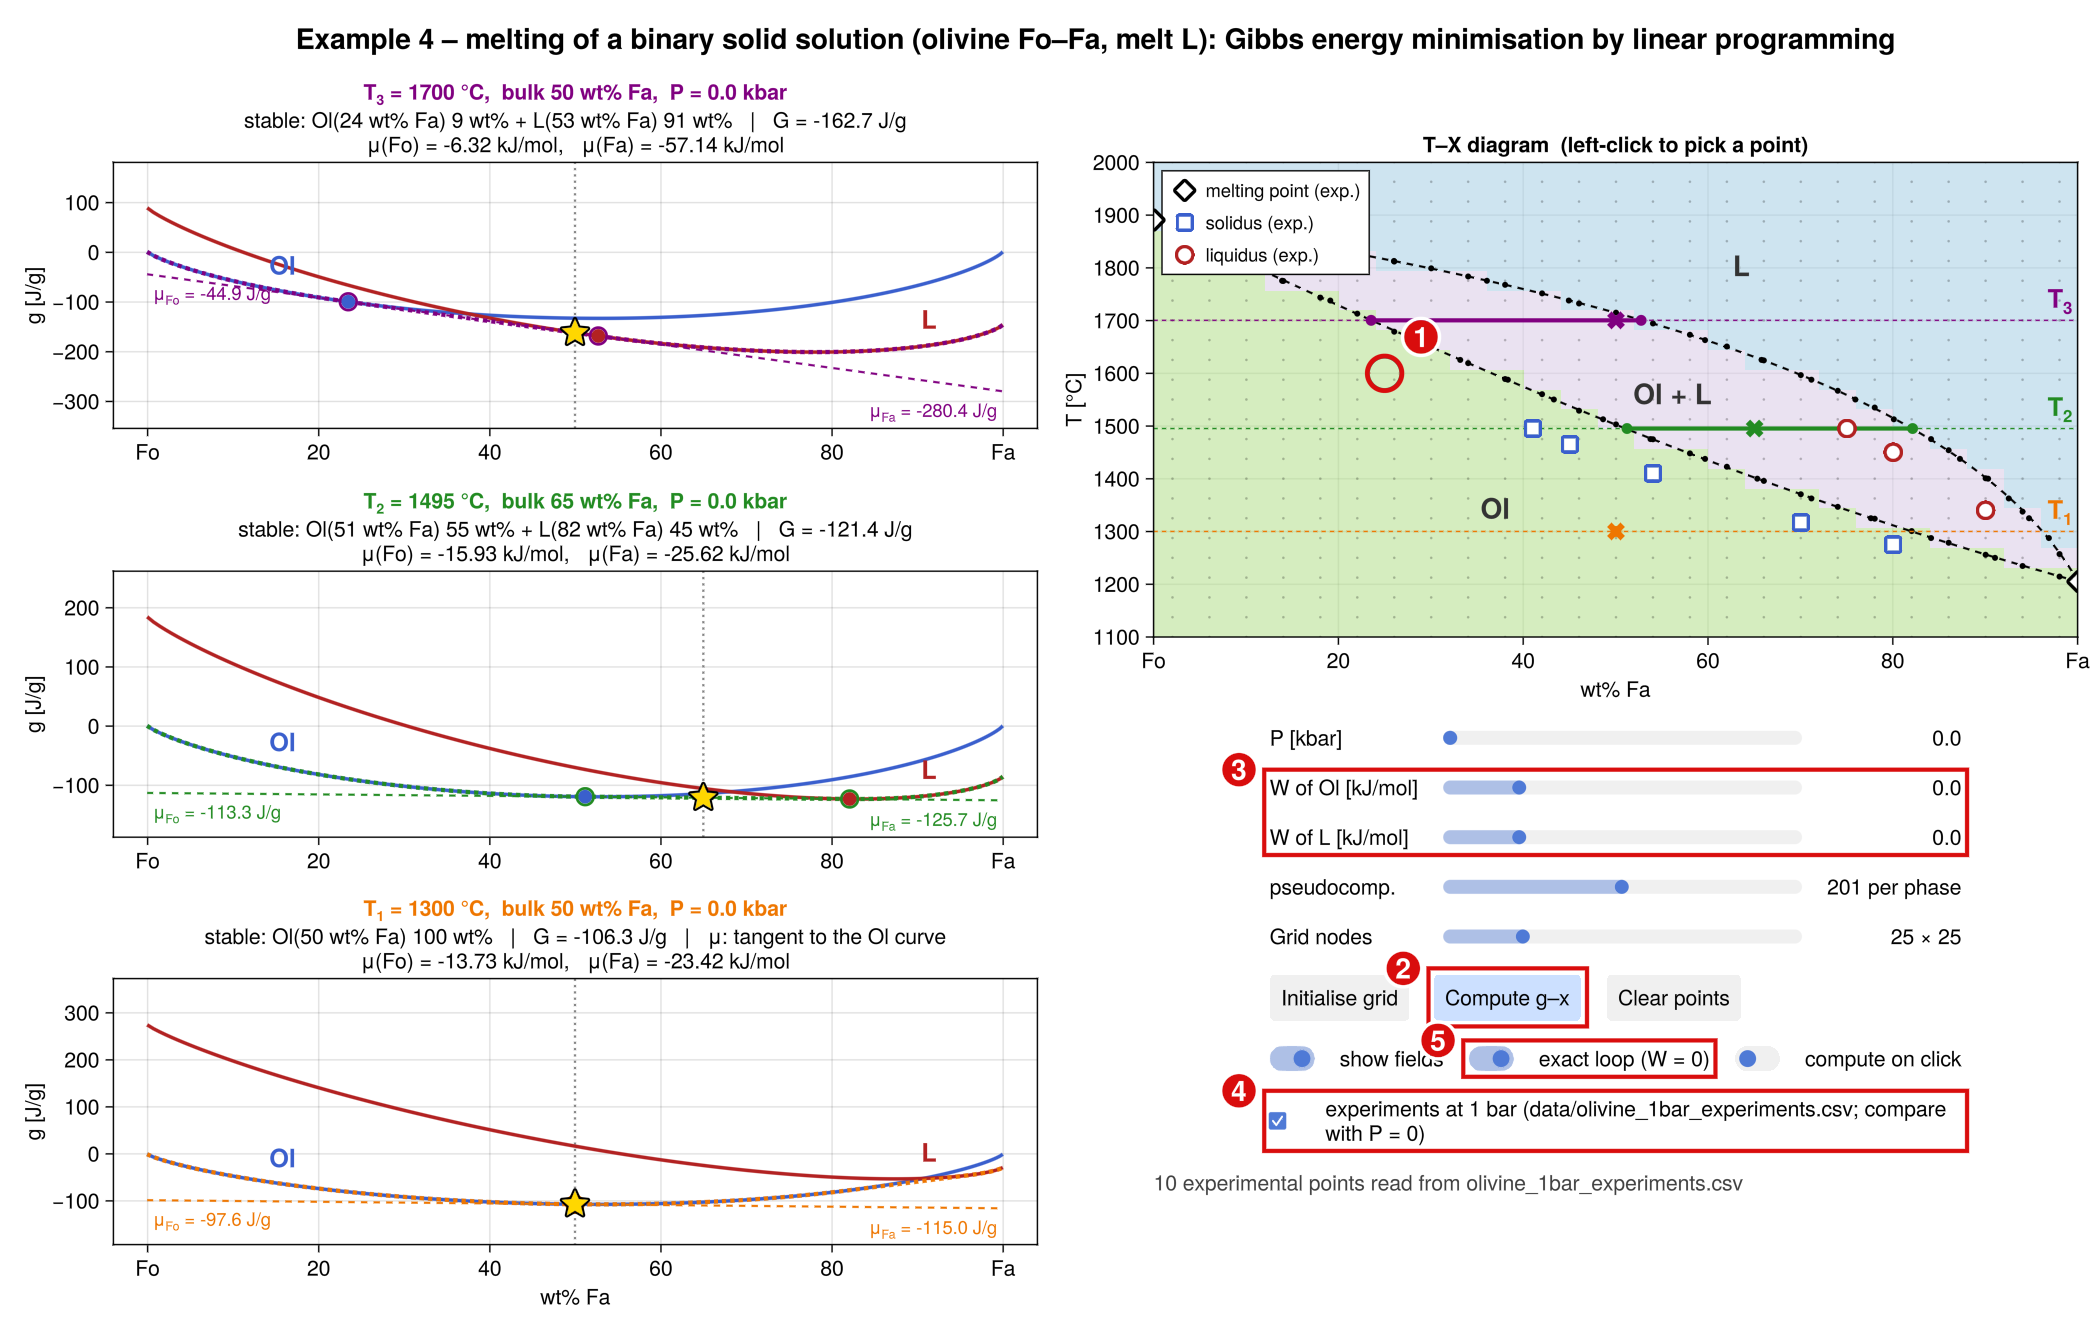
\includegraphics[width=\textwidth]{figures/ex4_overview.png}
\caption{Example 4 with three points and the experimental data at 1\,bar switched on.}
\label{fig:ex4}
\end{figure}

\paragraph{Step by step} (numbers as in Fig.~\ref{fig:ex4})
\begin{enumerate}[label=\protect\step{\arabic*}]
\item \textbf{Left-click} in the $T$–$X$ diagram.
\item \btn{Compute g–x}: the $g$–$x$ diagram shows the olivine (blue) and melt (red) curves and their common
  tangent; the tie-line olivine–melt is drawn in the $T$–$X$ diagram.
\item \ctl{W of Ol} and \ctl{W of L}: non-ideal solutions.
\item Check box \ctl{experiments at 1 bar}: shows the measurements stored in the file
  \file{data/\allowbreak olivine\_1bar\_\allowbreak experiments.csv} (blue squares: olivine/solidus, red circles: melt/liquidus,
  diamonds: melting points). Compare them with the model at $P = 0$.
\item \ctl{exact loop (W = 0)}: the closed-form solidus and liquidus.
\end{enumerate}

\paragraph{The data file.} One row per measurement: \texttt{T\_C, type, Fa, unit, source}, with
\texttt{type} = \texttt{liquidus}, \texttt{solidus} or \texttt{melting} and \texttt{unit} = \texttt{wt} or
\texttt{mol}; mole per cent are converted to weight per cent for the plot. Lines starting with \# are comments. The file is
read again every time the box is ticked, so you can add data while the program runs.

\begin{figure}[H]
\centering
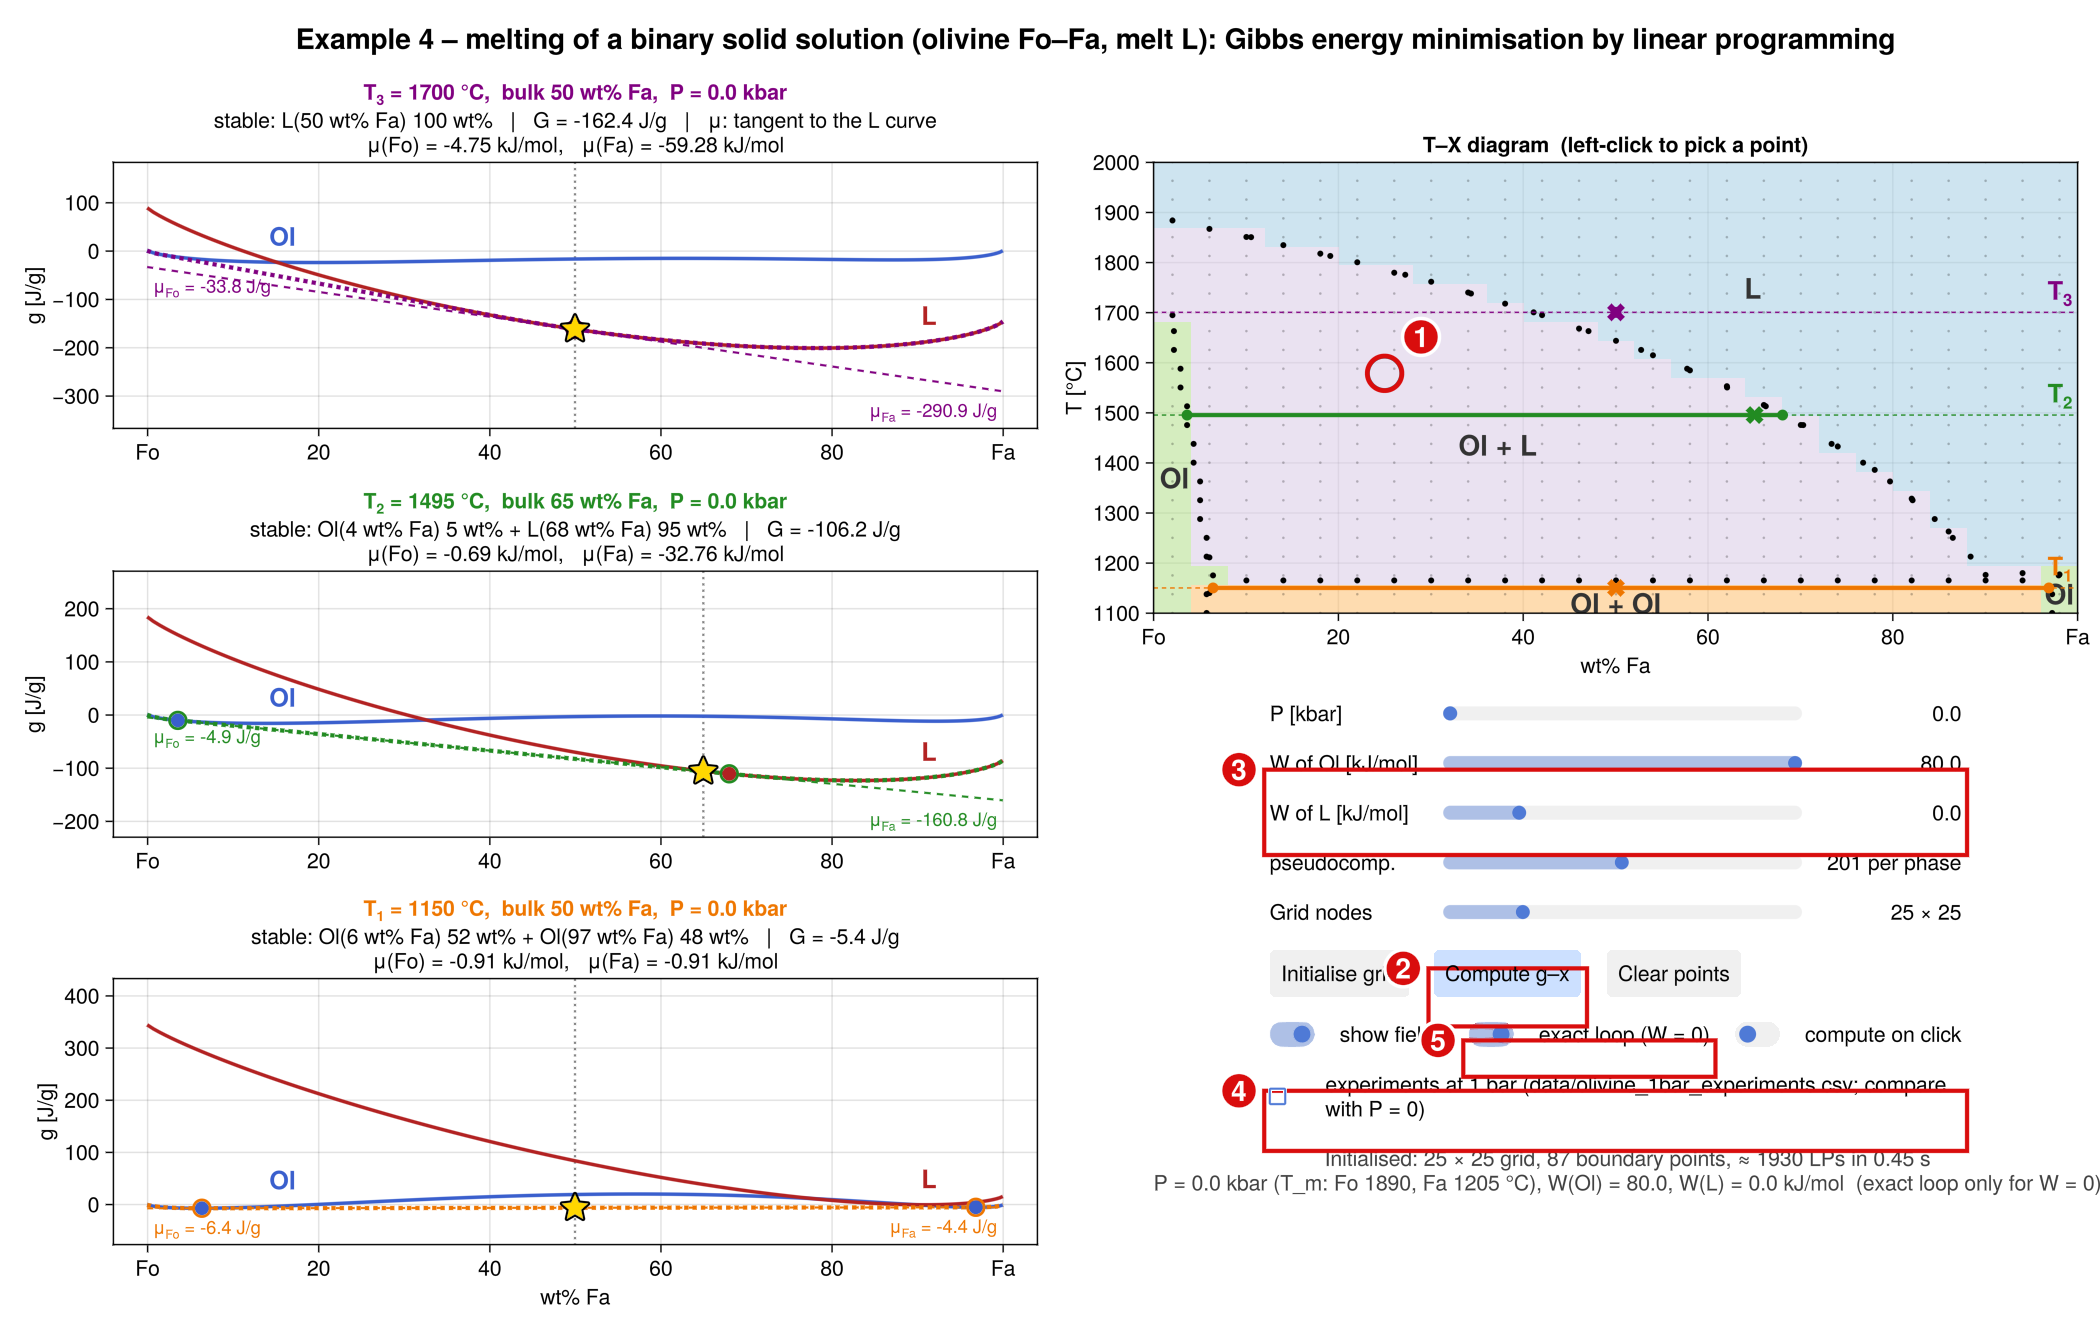
\includegraphics[width=0.75\textwidth]{figures/ex4_W80.png}
\caption{\ctl{W of Ol} = 80\,kJ/mol: a solvus Ol + Ol cuts the loop, which becomes a eutectic-like diagram.}
\end{figure}

\begin{tryit}
\begin{itemize}
\item Compare the model with the experiments. With the literature $\Delta H$ the model loop lies about
  8\,wt\% too far on the Fa side. In the USER INPUT block (\lstinline{MELTING}), try
  $\Delta H_\mathrm{Fo} = 120.5$ and $\Delta H_\mathrm{Fa} = 116.5$\,kJ/mol, which fit the data with an rms misfit of
  about 1.1\,wt\% (largest deviation about 2\,wt\%).
\item Increase \ctl{W of Ol} step by step (20, 40, 60, 80): where does the minimum and then the solvus appear?
\item Use 11 pseudocompounds and compare the LP boundaries with the exact loop.
\end{itemize}
\end{tryit}

%==============================================================================
\clearpage
\section{Example 5 – the ternary Di–An–Fo}\label{sec:ex5}
%==============================================================================
\textbf{File:} \file{Example5\_ternary\_DiAnFo.jl}.\quad
\textbf{Phases:} the pure solids diopside (Di), anorthite (An) and forsterite (Fo) and a melt. The
calculation is in moles (mole fractions $x_i$ of Di, An and Fo, $g$ in kJ/mol). The triangle, the phase
compositions and the amounts are shown in wt\%, as in the Di–An–Fo liquidus diagram of the course, and the 3D
view shows $g$ per gram (J/g) over the wt\% triangle, so that the tangent plane is a plane
(Section~\ref{sec:weight}). The melt has an effective number $q_i$ of mixing units per formula unit (the unit
fractions $y_i = q_i x_i / \sum_j q_j x_j$ take the place of the mole fractions in the mixing terms) and
asymmetric excess terms. Its parameters were \emph{calibrated} against the diagram:

\begin{table}[H]
\centering\small
\begin{tabular}{@{}lll@{}}
\toprule
 & model & diagram \\ \midrule
Di–An eutectic & 1274\,$^\circ$C, An 41.7\,wt\% & 1274\,$^\circ$C, An 42\,wt\% \\
Di–Fo eutectic & 1382\,$^\circ$C, Fo 12.1\,wt\% & 1387\,$^\circ$C, Fo 12.4\,wt\% \\
An–Fo eutectic & 1329\,$^\circ$C, Fo 28.3\,wt\% & 1327\,$^\circ$C, Fo 28.3\,wt\% \\
ternary eutectic & 1269\,$^\circ$C, Di49 An44 Fo07 & 1270\,$^\circ$C, Di49 An44 Fo07 \\
\bottomrule
\end{tabular}
\end{table}
\noindent The fitted enthalpies of fusion are \emph{effective} parameters, not measured values.

\begin{figure}[H]
\centering
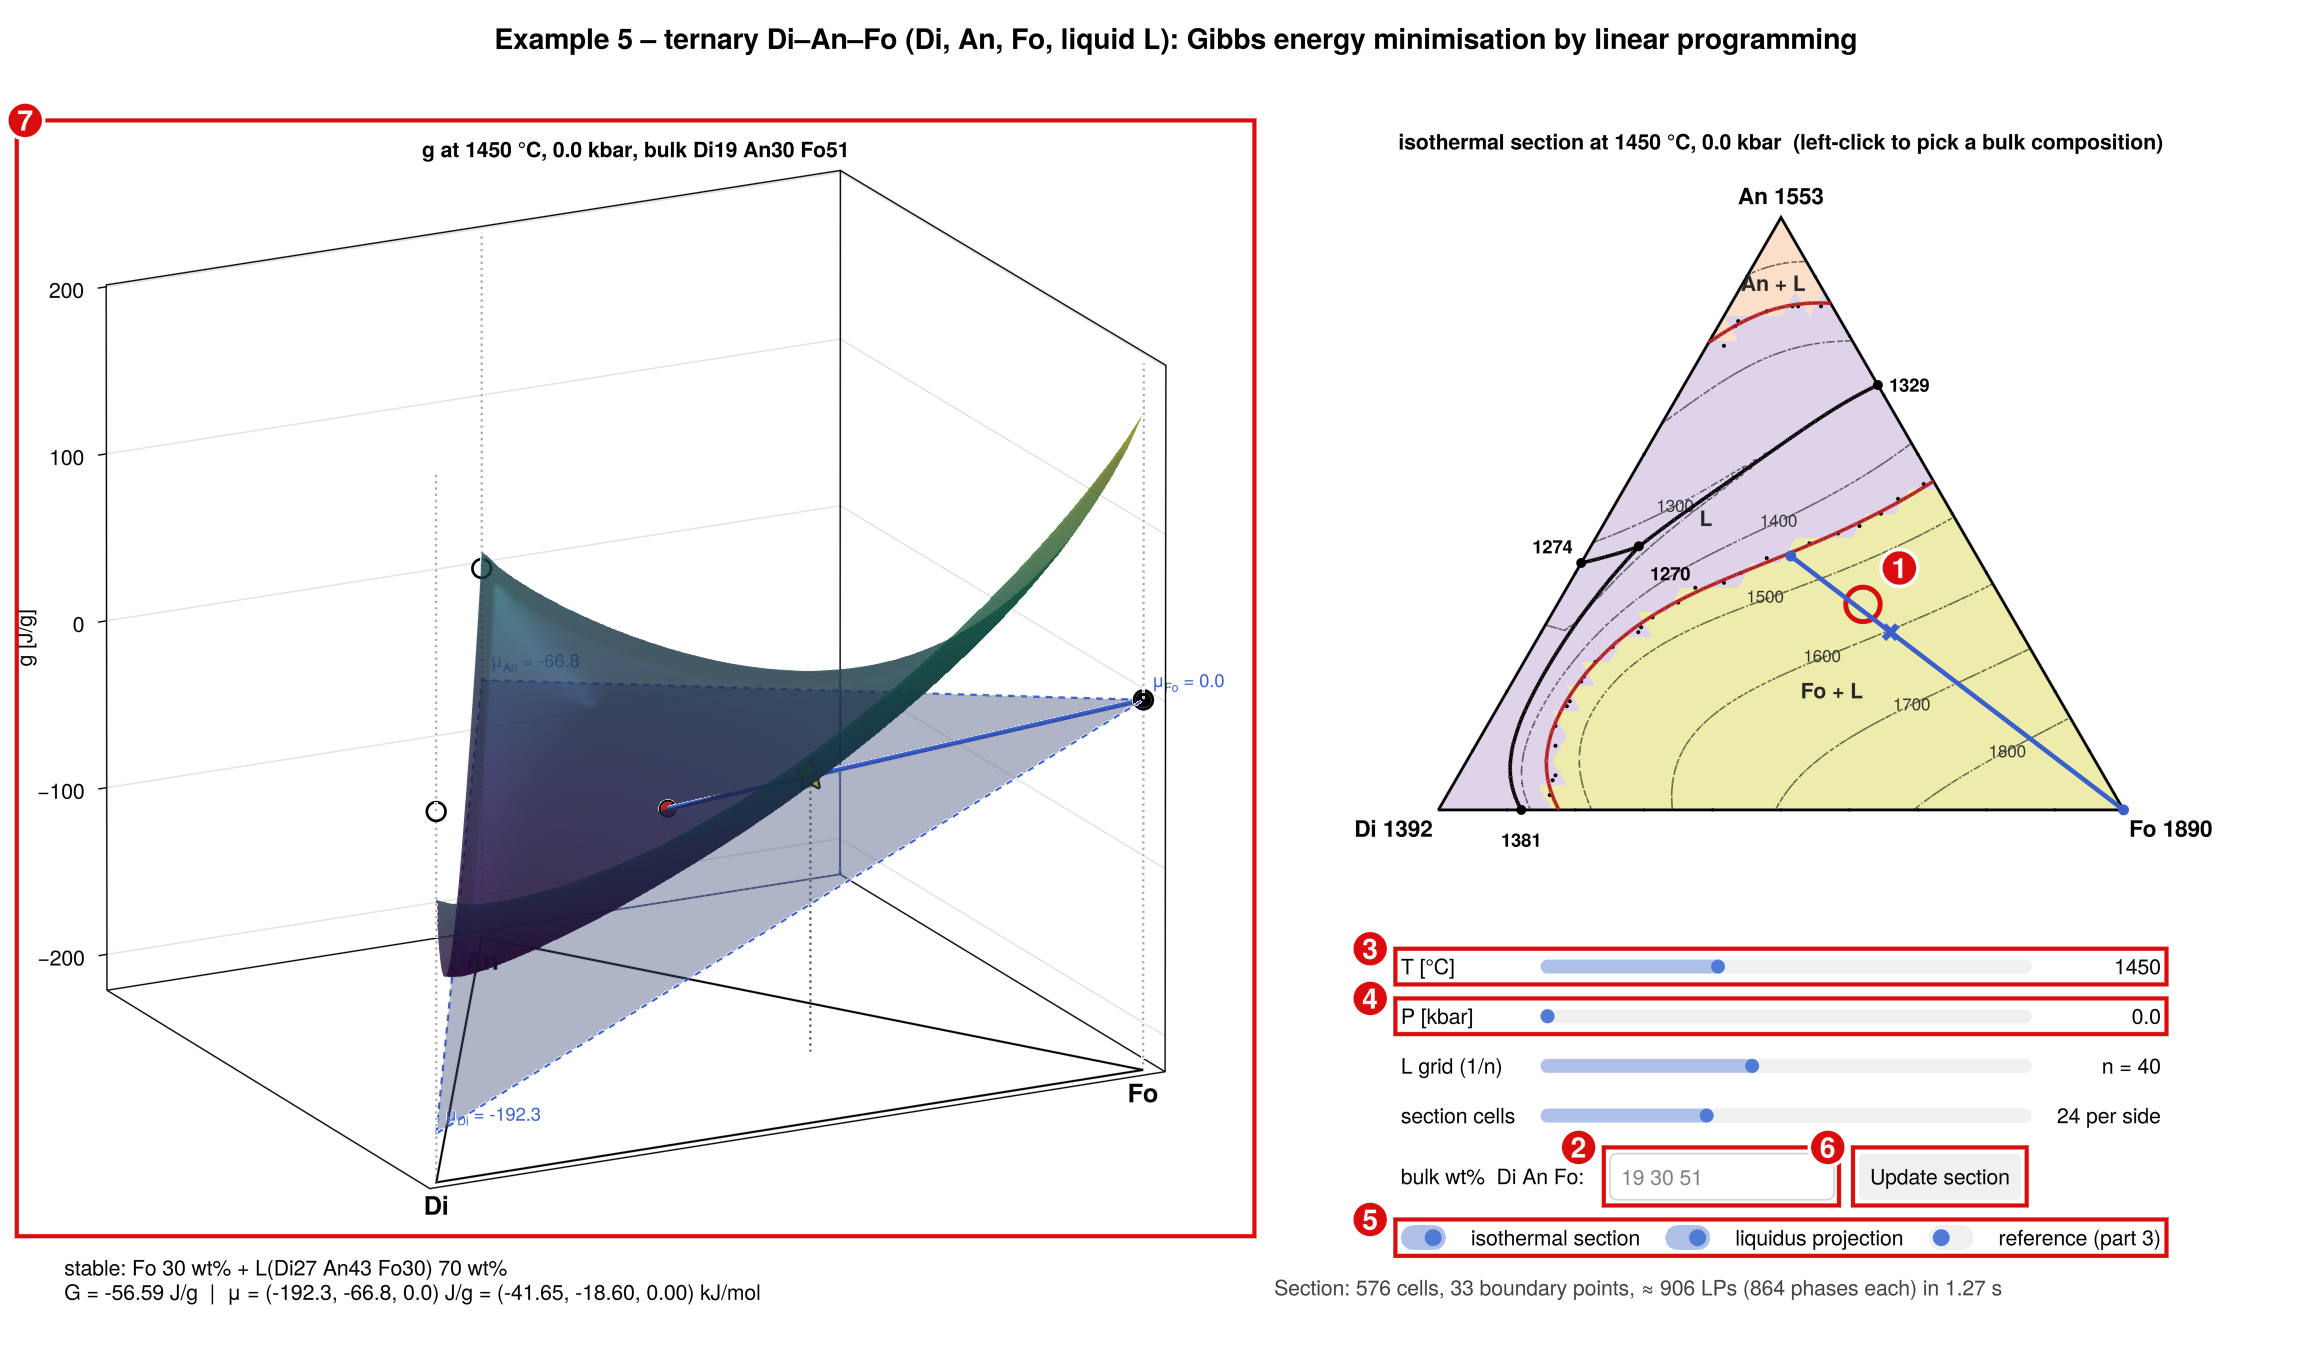
\includegraphics[width=\textwidth]{figures/ex5_overview.png}
\caption{Example 5 at 1450\,$^\circ$C with the bulk composition Di19 An30 Fo51 of the crystallization path in
the course: Fo + L, the melt has the composition Di27 An43 Fo30.}
\label{fig:ex5}
\end{figure}

\paragraph{Step by step} (numbers as in Fig.~\ref{fig:ex5})
\begin{enumerate}[label=\protect\step{\arabic*}]
\item \textbf{Left-click} inside the triangle to choose the bulk composition. The 3D view and the tie-line
  (or tie-triangle) are updated immediately; there is no compute button.
\item Or type the composition in wt\% into the box, e.g.\ \texttt{19 30 51} (Di An Fo), and press Enter.
\item \ctl{T [$^\circ$C]}: the 3D view follows immediately; the isothermal section is recomputed when you stop
  dragging (or press \btn{Update section}).
\item \ctl{P [kbar]}: moves all melting points (illustrative melting slopes).
\item Toggles: \ctl{isothermal section} (stable assemblage on a grid of bulk compositions, by LP; the red dashed
  line is the analytic liquidus isotherm at $T$), \ctl{liquidus projection} (primary fields, cotectics,
  eutectics and isotherms of the model) and \ctl{reference (part 3)} (cotectics, eutectics and the
  crystallization path read from the course diagram, in red).
\item \btn{Update section} recomputes the isothermal section, e.g.\ after changing \ctl{section cells}.
\item The 3D view: the $g$ surface of the melt over the composition triangle, the solids at $g = 0$, the tangent
  plane through the stable phases (its heights at the corners are $\mu_\mathrm{Di}$, $\mu_\mathrm{An}$,
  $\mu_\mathrm{Fo}$ per gram; the values in kJ/mol are printed below the view) and the bulk composition
  (star). Drag with the mouse to rotate.
\end{enumerate}

\begin{figure}[H]
\centering
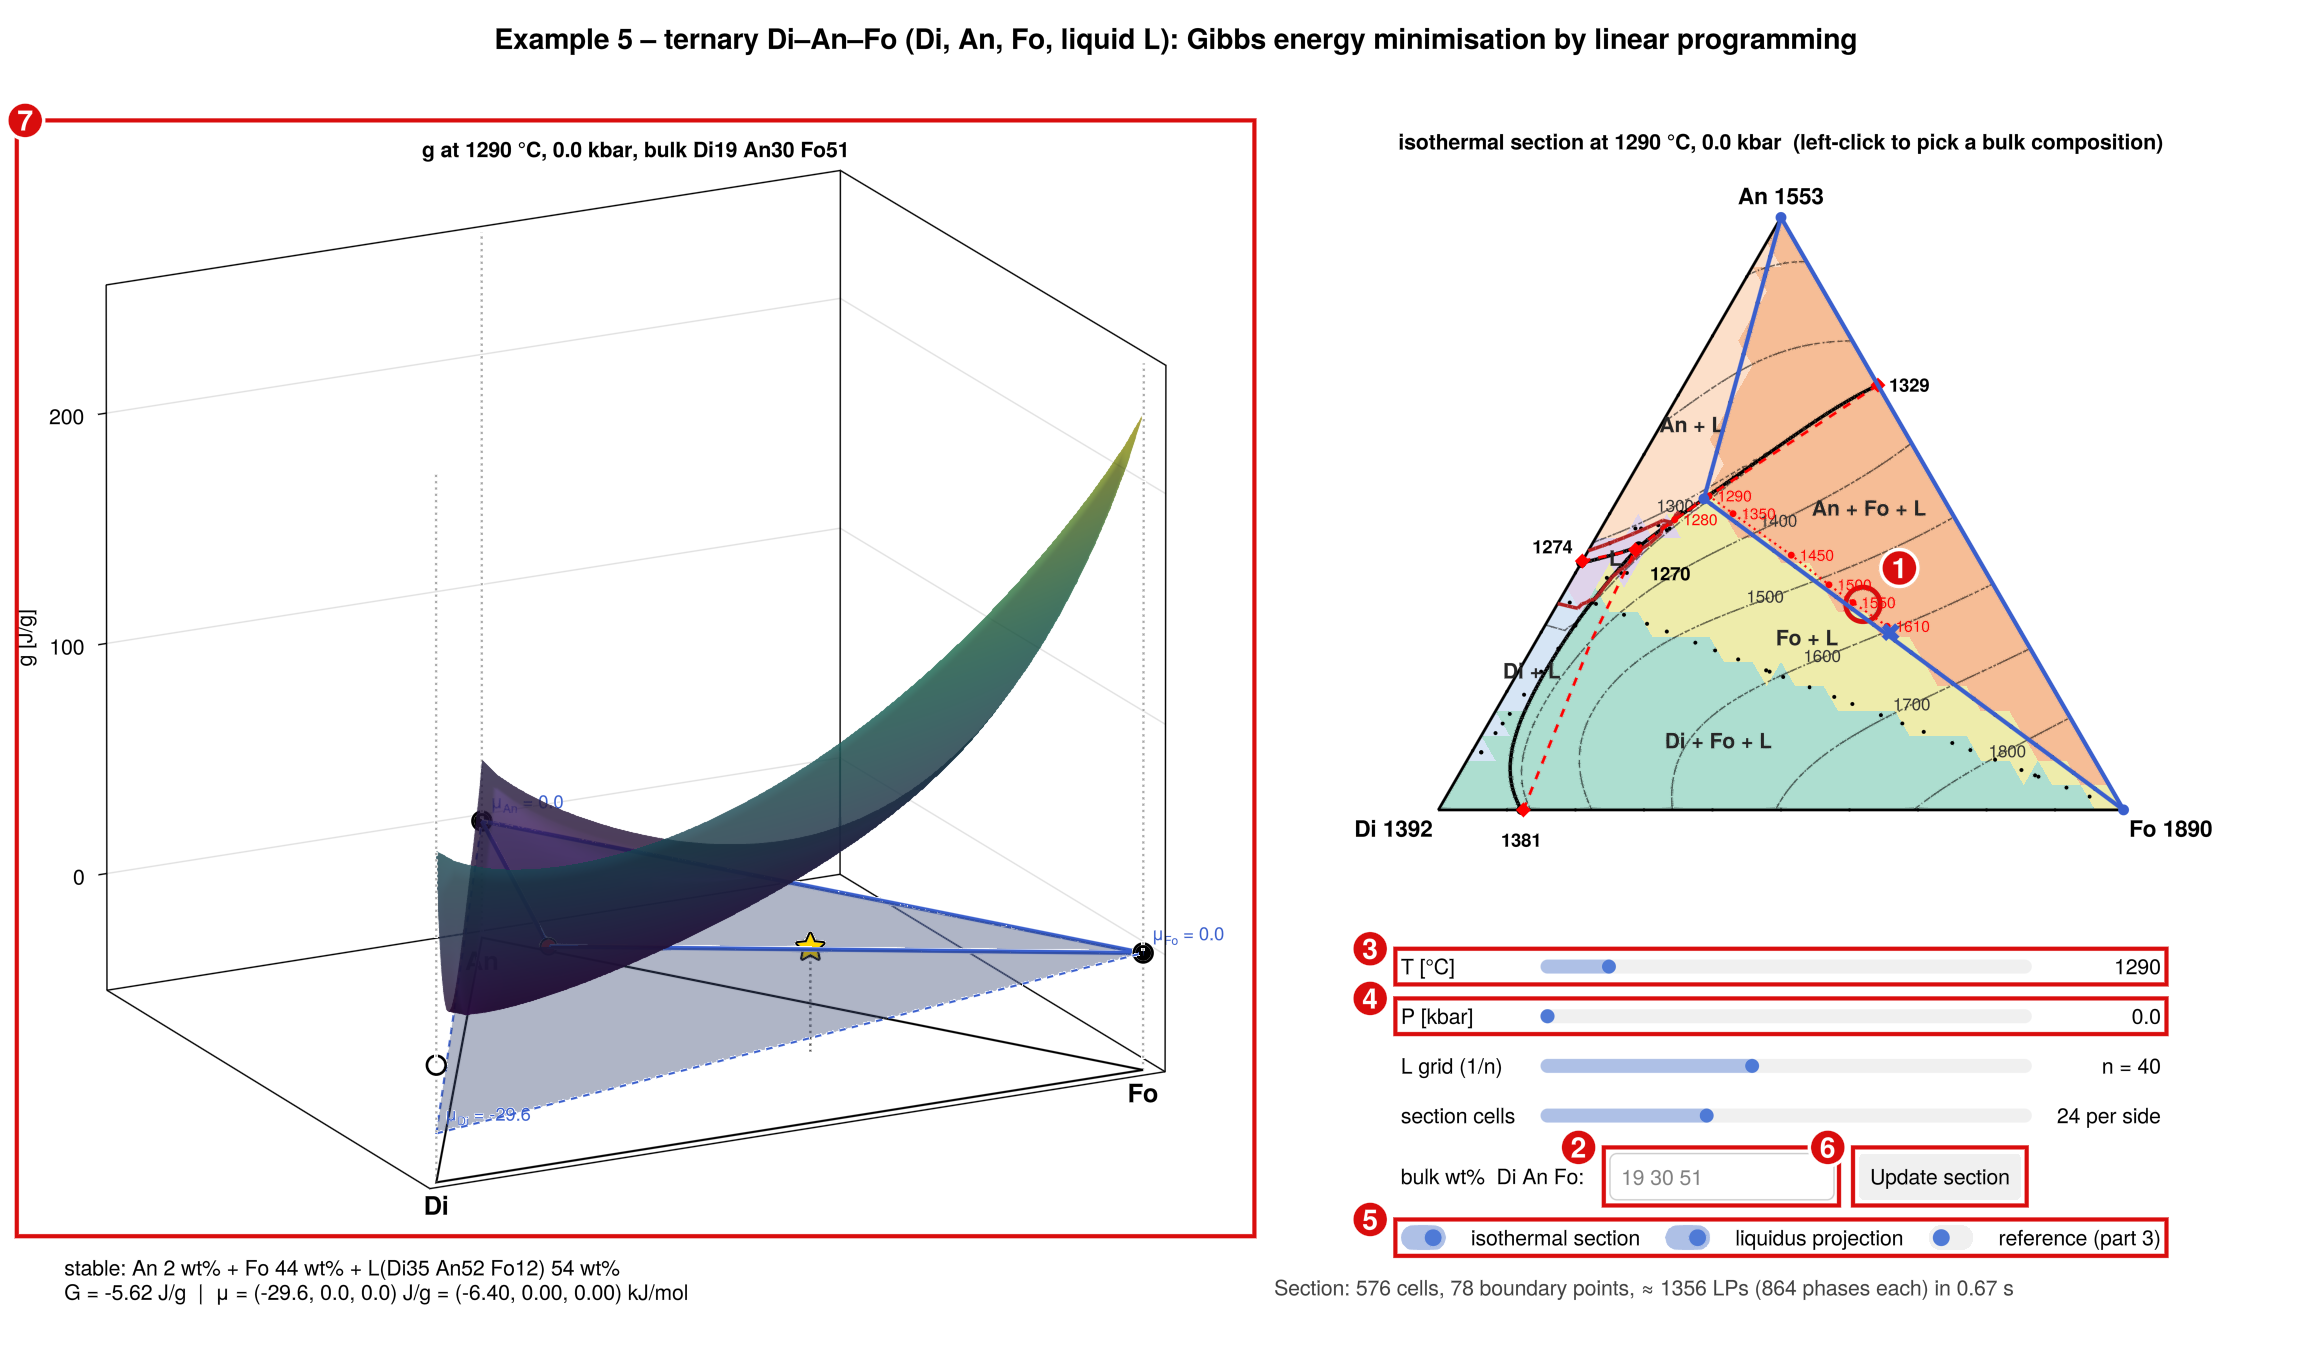
\includegraphics[width=0.49\textwidth]{figures/ex5_1290_reference.png}\hfill
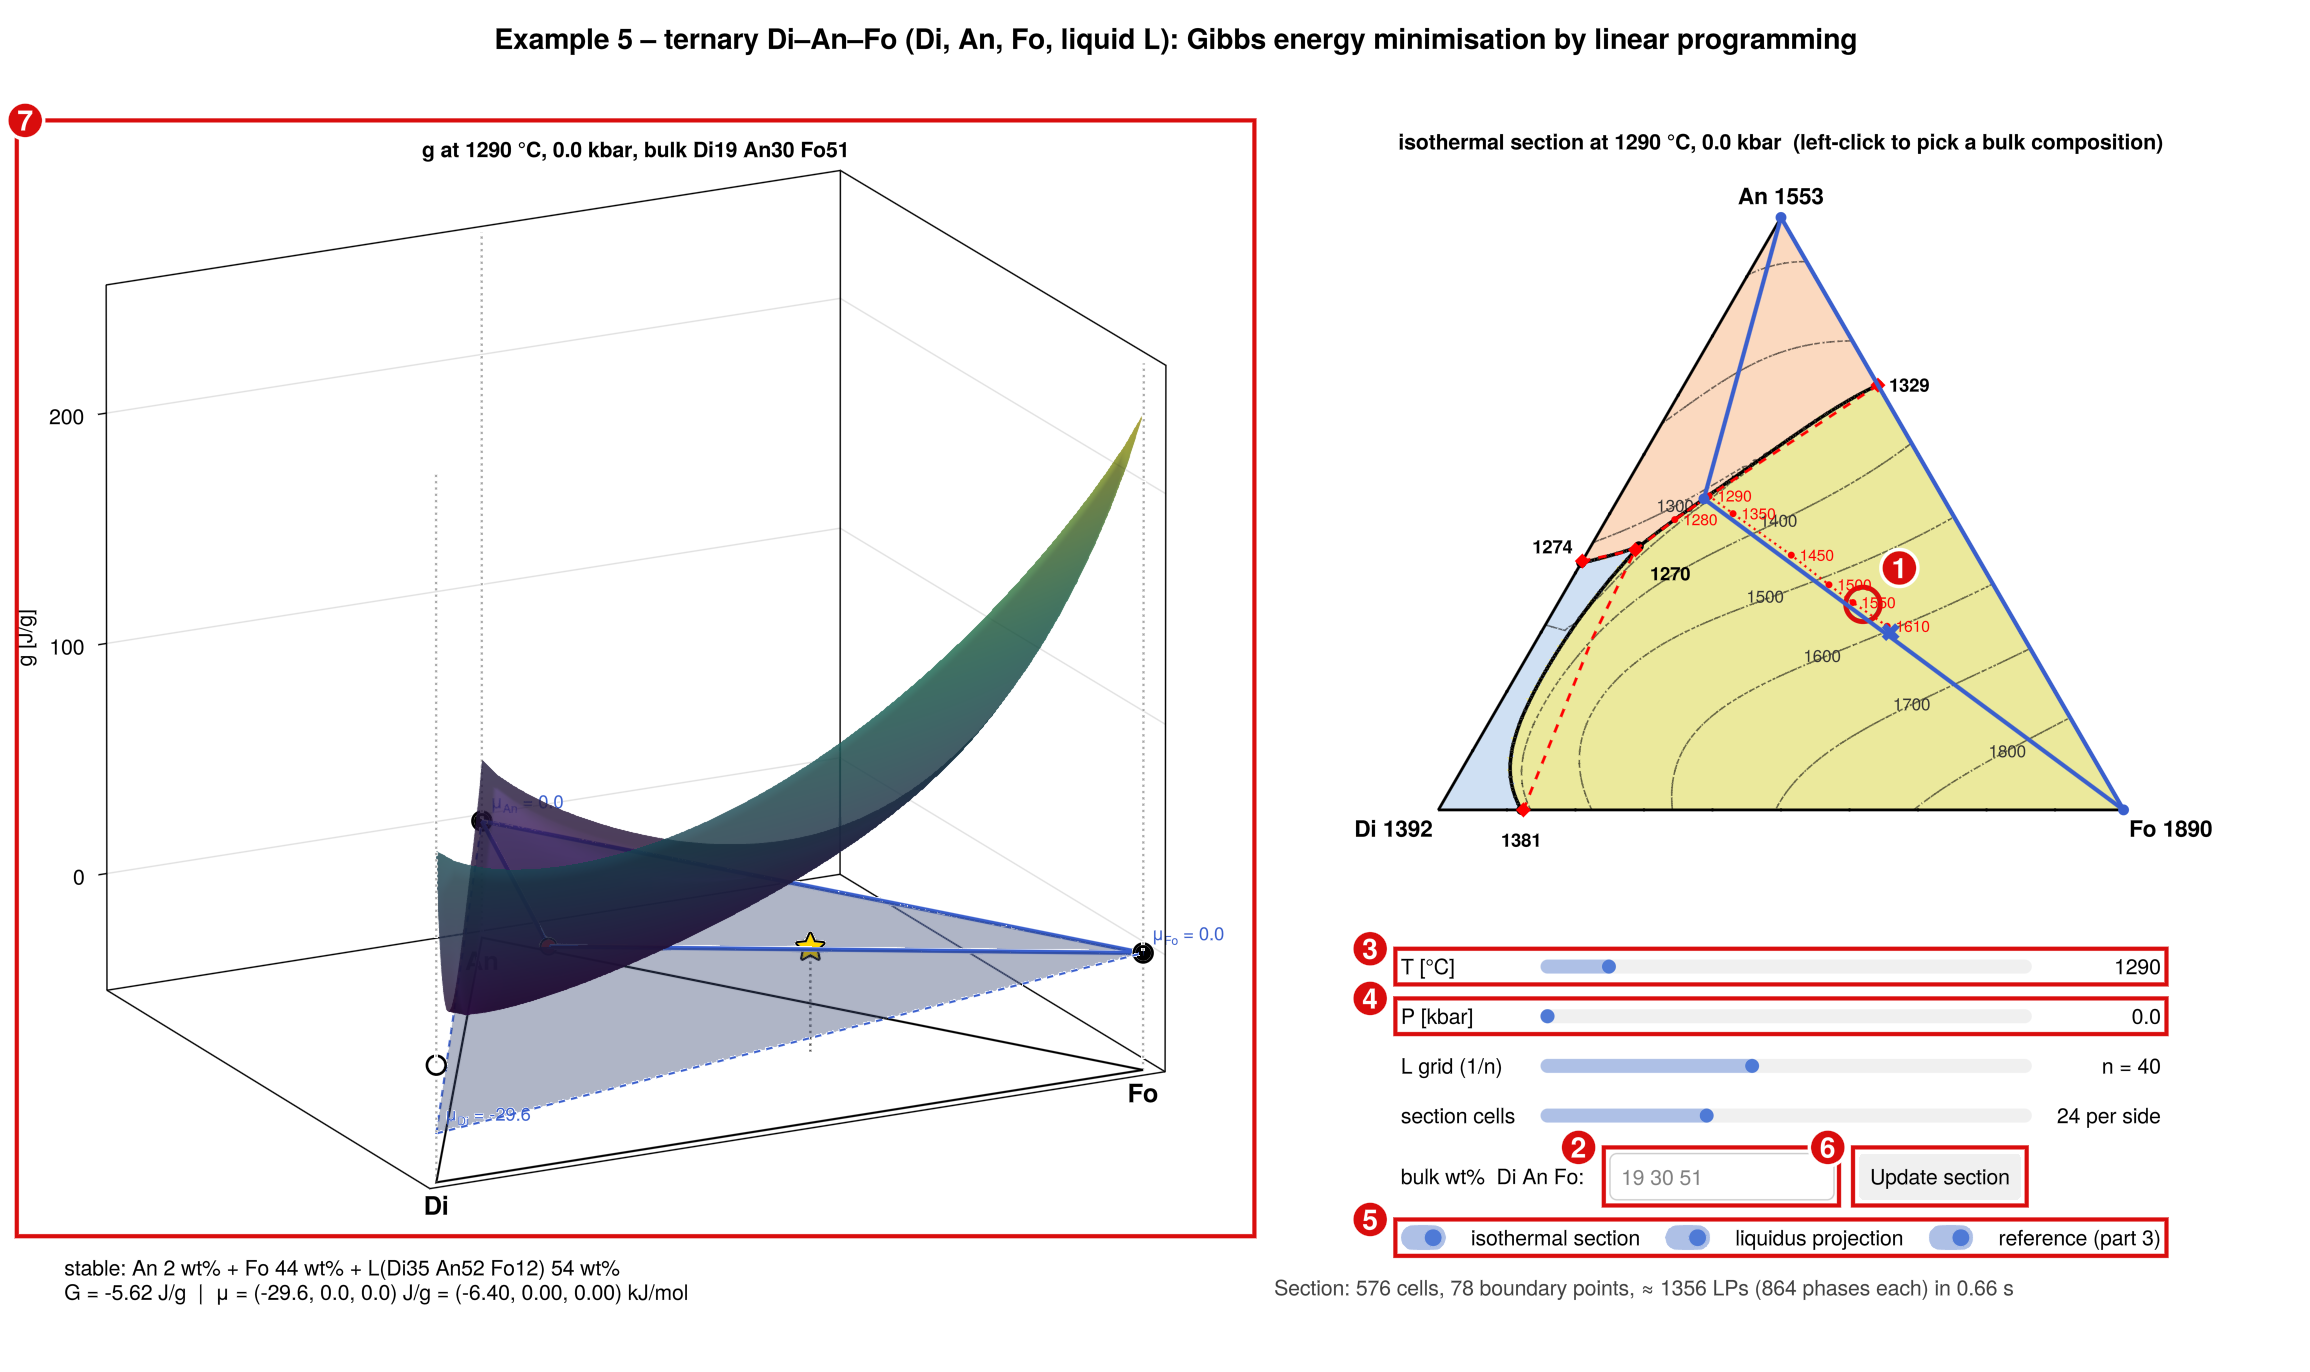
\includegraphics[width=0.49\textwidth]{figures/ex5_projection.png}
\caption{Left: 1290\,$^\circ$C with the reference switched on: the bulk lies in the three-phase triangle
An + Fo + L, the melt sits on the An–Fo cotectic. Right: the liquidus projection alone, compared with the
reference diagram.}
\end{figure}

\begin{tryit}
\begin{itemize}
\item Follow the crystallization path of Di19 An30 Fo51: set $T$ = 1610, 1550, 1500, 1450, 1350, 1290, 1280 and
  1265\,$^\circ$C and write down the melt composition and the amounts. Compare with the slides
  (e.g.\ 1450\,$^\circ$C: 70\% melt Di27 An43 Fo30 + 30\% Fo).
\item At 1290\,$^\circ$C two three-phase triangles exist (An + Fo + L and Di + Fo + L). Why, given the
  temperatures of the binary eutectics?
\item Rotate the 3D view until you look along the tangent plane: which phases touch it?
\end{itemize}
\end{tryit}

%==============================================================================
\clearpage
\section{Example 6 – the ternary CaO–Al\texorpdfstring{$_2$}{2}O\texorpdfstring{$_3$}{3}–SiO\texorpdfstring{$_2$}{2}}\label{sec:ex6}
%==============================================================================
\textbf{File:} \file{Example6\_ternary\_CAS.jl}.\quad
The same program as Example~5, but for a system whose corners are \emph{oxides} and whose solids are mostly
\emph{compounds} that lie inside the triangle or on its edges. The triangle is drawn in wt\% with CaO bottom
left, Al$_2$O$_3$ bottom right and SiO$_2$ at the top, as the liquidus projection of the course
(\file{data/Papers/CAS\_Ternary.png}). Compositions are written in cement notation, C = CaO, A = Al$_2$O$_3$,
S = SiO$_2$, e.g.\ C28 A16 S56 = 28\,wt\% CaO, 16\,wt\% Al$_2$O$_3$, 56\,wt\% SiO$_2$. There is no pressure
slider: the diagram is for 1\,atm, and at high pressure other phases (garnet, kyanite, \dots) appear that
are not in the model.

\begin{table}[H]
\centering\small
\caption{The solids of Example 6. ``Congruent'': the compound lies inside its own primary field and melts to a
liquid of its own composition; ``incongruent'': it lies outside its field and melts to another solid + liquid.}
\label{tab:cas}
\begin{tabular}{@{}llll@{}}
\toprule
key & phase & formula (notation) & melting \\ \midrule
Lime & lime & CaO (C) & 2572\,$^\circ$C \\
Crs, Trd & cristobalite, tridymite & SiO$_2$ (S) & 1723\,$^\circ$C (Crs); Trd stable below 1470\,$^\circ$C \\
Crn & corundum & Al$_2$O$_3$ (A) & 2054\,$^\circ$C \\
Pwo & pseudowollastonite & CaSiO$_3$ (CS) & congruent, 1544\,$^\circ$C \\
C2S & dicalcium silicate & Ca$_2$SiO$_4$ (C$_2$S) & congruent, 2130\,$^\circ$C \\
An & anorthite & CaAl$_2$Si$_2$O$_8$ (CAS$_2$) & congruent, 1553\,$^\circ$C \\
Gh & gehlenite & Ca$_2$Al$_2$SiO$_7$ (C$_2$AS) & congruent, 1593\,$^\circ$C \\
Mul & mullite & Al$_6$Si$_2$O$_{13}$ (A$_3$S$_2$) & congruent, 1890\,$^\circ$C \\
CA, CA2 & calcium aluminates & CaAl$_2$O$_4$, CaAl$_4$O$_7$ & congruent, 1604 and 1765\,$^\circ$C \\
CA6 & hibonite & CaAl$_{12}$O$_{19}$ & incongruent (Crn + L) \\
C3A & tricalcium aluminate & Ca$_3$Al$_2$O$_6$ & incongruent (Lime + L) \\
\bottomrule
\end{tabular}
\end{table}

\paragraph{The model.} The calculation is in moles of the oxides ($x_i$ = mole fractions of CaO, Al$_2$O$_3$,
SiO$_2$; $g$ in kJ per mole of oxides). The reference states are the pure oxide \emph{liquids} ($g = 0$). As in
Example~5 the liquid mixes $q_i$ ``mixing units'' per mole of oxide $i$ (unit fractions
$y_i = q_i x_i/\sum_j q_j x_j$, $\nu = \sum_j q_j x_j$),
\begin{equation}\label{eq:casliq}
  g_L(x, T) = \nu\Big[RT\sum_i y_i\ln y_i + \sum_m \big(W_{H,m} - T\,W_{S,m}\big)\prod_i y_i^{e_{m,i}}\Big],
\end{equation}
with 26 excess terms (powers $e_m$ of degree 3 to 5; the fit gives an appreciable entropy part $W_S$ only to the
seven terms of degree 3, the others are kept almost purely enthalpic).
Every \emph{solid} $s$ with the oxide mole fractions $c_s$ is defined from the liquid of the \emph{same}
composition and a fusion term, Eq.~\eqref{eq:melt}:
\begin{equation}\label{eq:cassol}
  g_s(T) = g_L(c_s, T) - \Delta H_s\left(1 - \frac{T}{T_{m,s}}\right).
\end{equation}
A compound that melts congruently therefore melts exactly at its melting point $T_{m,s}$, whatever the liquid
model is. For CA6 and C3A, which melt incongruently, $T_{m,s}$ is a fitted melting point that is never
reached (the compound breaks down first). Tridymite is cristobalite with
$g_\mathrm{Trd} - g_\mathrm{Crs} = -\Delta H_t\,(1 - T/T_t)$, $T_t = 1470\,^\circ$C. All $g$ are again of the
form \eqref{eq:g}, so the linear programme is the same as before: 13 solids and 861 liquid pseudocompounds.

\paragraph{Liquidus.} Solid $s$ is saturated in a liquid of composition $x$ when
$\sum_i c_{s,i}\,\mu_i^L(x, T) = g_s(T)$. Both sides are linear in $T$ ($\mu_i^L = A_i(x) - T\,B_i(x)$), so the
liquidus temperature of every solid has a closed form,
\begin{equation}\label{eq:castl}
  T_s(x) = \frac{\sum_i c_{s,i} A_i(x) - h_s}{\sum_i c_{s,i} B_i(x) - s_s},
\end{equation}
and the liquidus is the highest of them. The liquidus projection (primary fields, field boundaries, isotherms,
invariant points) is computed from Eq.~\eqref{eq:castl}; the isothermal sections come from the LP.

\paragraph{Calibration.} {\sloppy The liquidus projection of the course was digitised
(\file{data/\allowbreak CAS\_liquidus\_\allowbreak digitized.txt}): 13 ternary invariant points, 11 points on
the edges, the labelled isotherms and one point inside every primary field. The figure gives no temperatures
for the invariant points; they are taken from Osborn and Muan (1960) and, for CaO–Al$_2$O$_3$, from Jerebtsov
and Mikhailov (2001). The digitised compositions agree with Osborn and Muan to about 1\,wt\%. The program
\file{calibration/\allowbreak fit\_Example6\_CAS.jl} fits $q$, the excess terms, the $\Delta H_s$ and the two
metastable melting points (Levenberg–Marquardt, no packages needed); a penalty keeps the liquid stable
(convex $g$, no unmixing) on a grid of compositions. The script prints the parameter block for the USER INPUT
section of the example.\par}
\begin{table}[H]
\centering\small
\begin{tabular}{@{}lll@{}}
\toprule
 & model & Osborn \& Muan (1960) \\ \midrule
An + Pwo + Trd (eutectic) & 1182\,$^\circ$C, C24 A14 S61 & 1170\,$^\circ$C, C23 A15 S62 \\
An + Gh + Pwo (eutectic)  & 1279\,$^\circ$C, C37 A21 S42 & 1265\,$^\circ$C, C38 A20 S42 \\
An + Mul + Trd            & 1332\,$^\circ$C, C12 A21 S68 & 1345\,$^\circ$C, C10 A20 S70 \\
An + Mul + Crn            & 1483\,$^\circ$C, C15 A34 S52 & 1512\,$^\circ$C, C16 A37 S48 \\
C2S + CA + C3A            & 1336\,$^\circ$C, C49 A44 S7  & 1335\,$^\circ$C, C50 A44 S7 \\
\midrule
all 13 ternary + 11 edge points & \multicolumn{2}{l}{rms 27\,K, max 86\,K; liquid compositions rms 3\,wt\%} \\
\bottomrule
\end{tabular}
\end{table}
\noindent Every primary field of the figure is reproduced, except two very narrow fields that were left
out: Ca$_3$SiO$_5$ (between lime and C2S) and rankinite Ca$_3$Si$_2$O$_7$ (between C2S and Pwo). The fitted
$\Delta H_s$ are \emph{effective} parameters, not calorimetric values.

\begin{note}
The real CaO–SiO$_2$ liquid unmixes near SiO$_2$: two liquids above about 1690\,$^\circ$C, as in the
MgO–SiO$_2$ system of Example~3. This is why the cristobalite isotherms of the figure (1600 and 1700\,$^\circ$C)
are so flat next to the CaO–SiO$_2$ edge. The model has no two-liquid field, so its cristobalite liquidus
there is 100–200\,K too low. The lime liquidus at the Lime–C2S boundary is about 85\,K too low.
\end{note}

\begin{figure}[H]
\centering
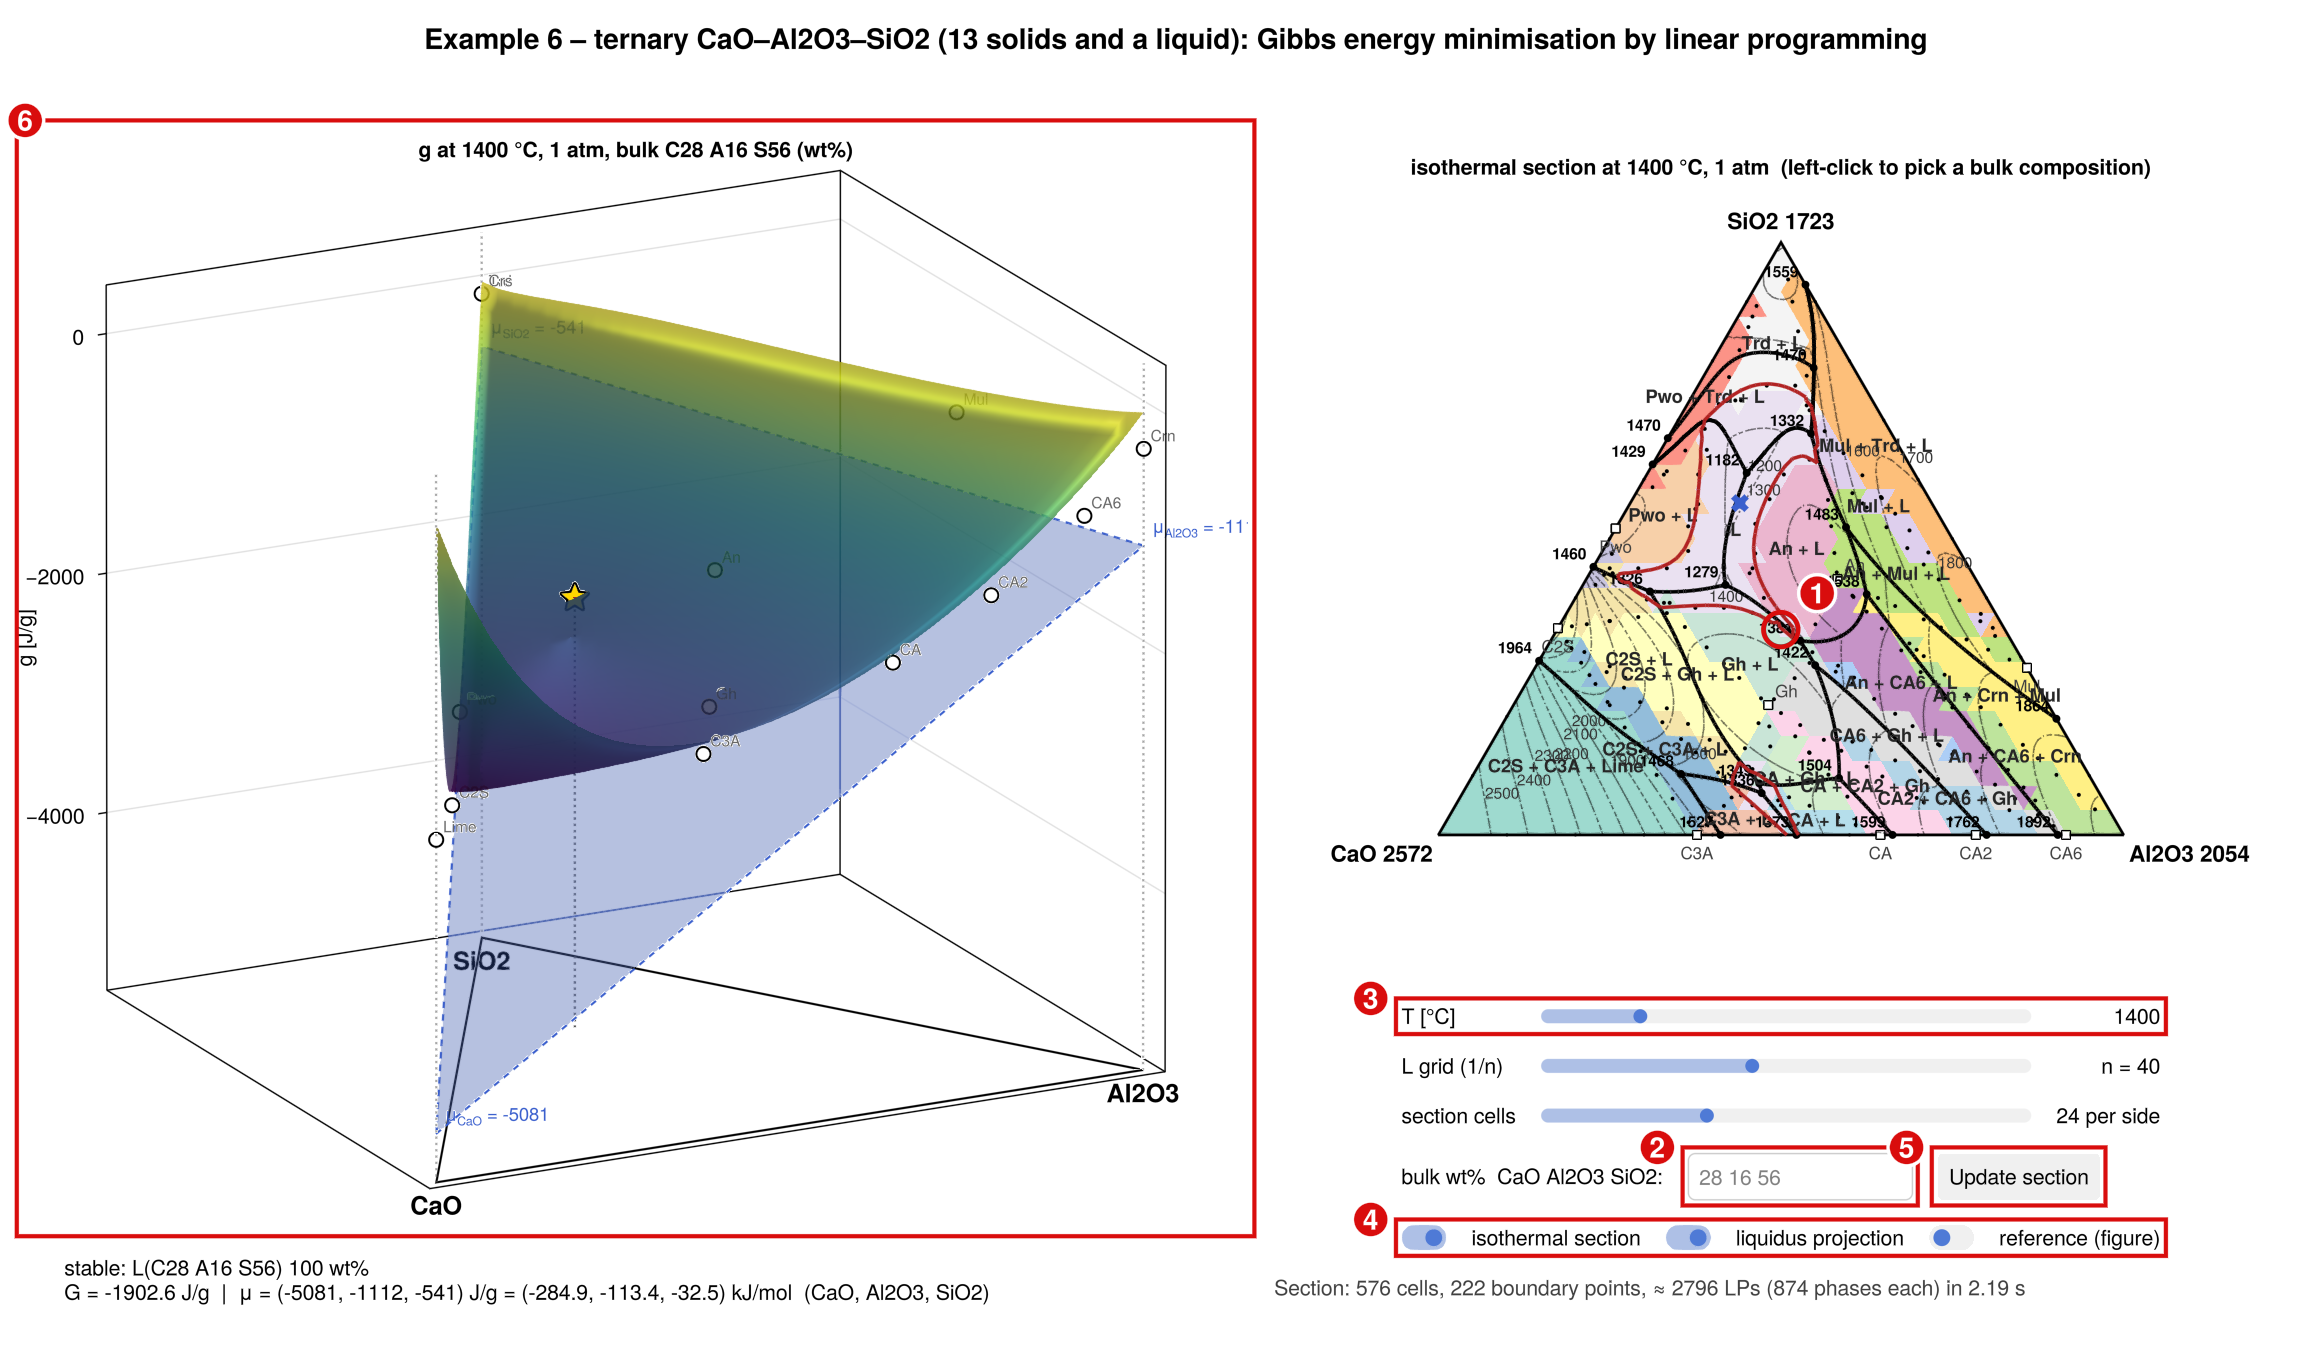
\includegraphics[width=\textwidth]{figures/ex6_overview.png}
\caption{Example 6 at 1400\,$^\circ$C with the bulk composition C28 A16 S56 (the green dot of the course
figure): the bulk is completely molten. The isothermal section is coloured; the black lines are the liquidus
projection of the model, the red dashed line the liquidus isotherm at 1400\,$^\circ$C.}
\label{fig:ex6}
\end{figure}

\paragraph{Step by step} (numbers as in Fig.~\ref{fig:ex6})
\begin{enumerate}[label=\protect\step{\arabic*}]
\item \textbf{Left-click} inside the triangle to choose the bulk composition. The 3D view and the tie-line
  (or tie-triangle) are updated immediately; there is no compute button.
\item Or type the composition in wt\% into the box, e.g.\ \texttt{28 16 56} (CaO Al$_2$O$_3$ SiO$_2$), and
  press Enter.
\item \ctl{T [$^\circ$C]} (1100–2650\,$^\circ$C): the 3D view follows immediately; the isothermal section is
  recomputed when you stop dragging (or press \btn{Update section}).
\item Toggles: \ctl{isothermal section} (stable assemblage on a grid of bulk compositions, by LP),
  \ctl{liquidus projection} (primary fields, field boundaries, isotherms and invariant points of the model,
  with their temperatures) and \ctl{reference (figure)} (the course figure is drawn underneath, with the
  invariant points used for the calibration and their literature temperatures in red).
\item \btn{Update section} recomputes the isothermal section, e.g.\ after changing \ctl{section cells}.
\item The 3D view: the $g$ surface of the liquid over the composition triangle (per gram, over the wt\%
  triangle), the solids as dots at their own composition (black: stable), the tangent plane through the
  stable phases (its heights at the corners are $\mu_\mathrm{CaO}$, $\mu_\mathrm{Al_2O_3}$,
  $\mu_\mathrm{SiO_2}$ per gram; the values in kJ/mol are printed below the view) and the bulk composition
  (star). Drag with the mouse to rotate.
\end{enumerate}
The open squares in the triangle mark the compositions of the compounds. A congruently melting compound lies
inside its own field (e.g.\ An, Gh, Mul); CA6 and C3A lie outside theirs.

\begin{figure}[H]
\centering
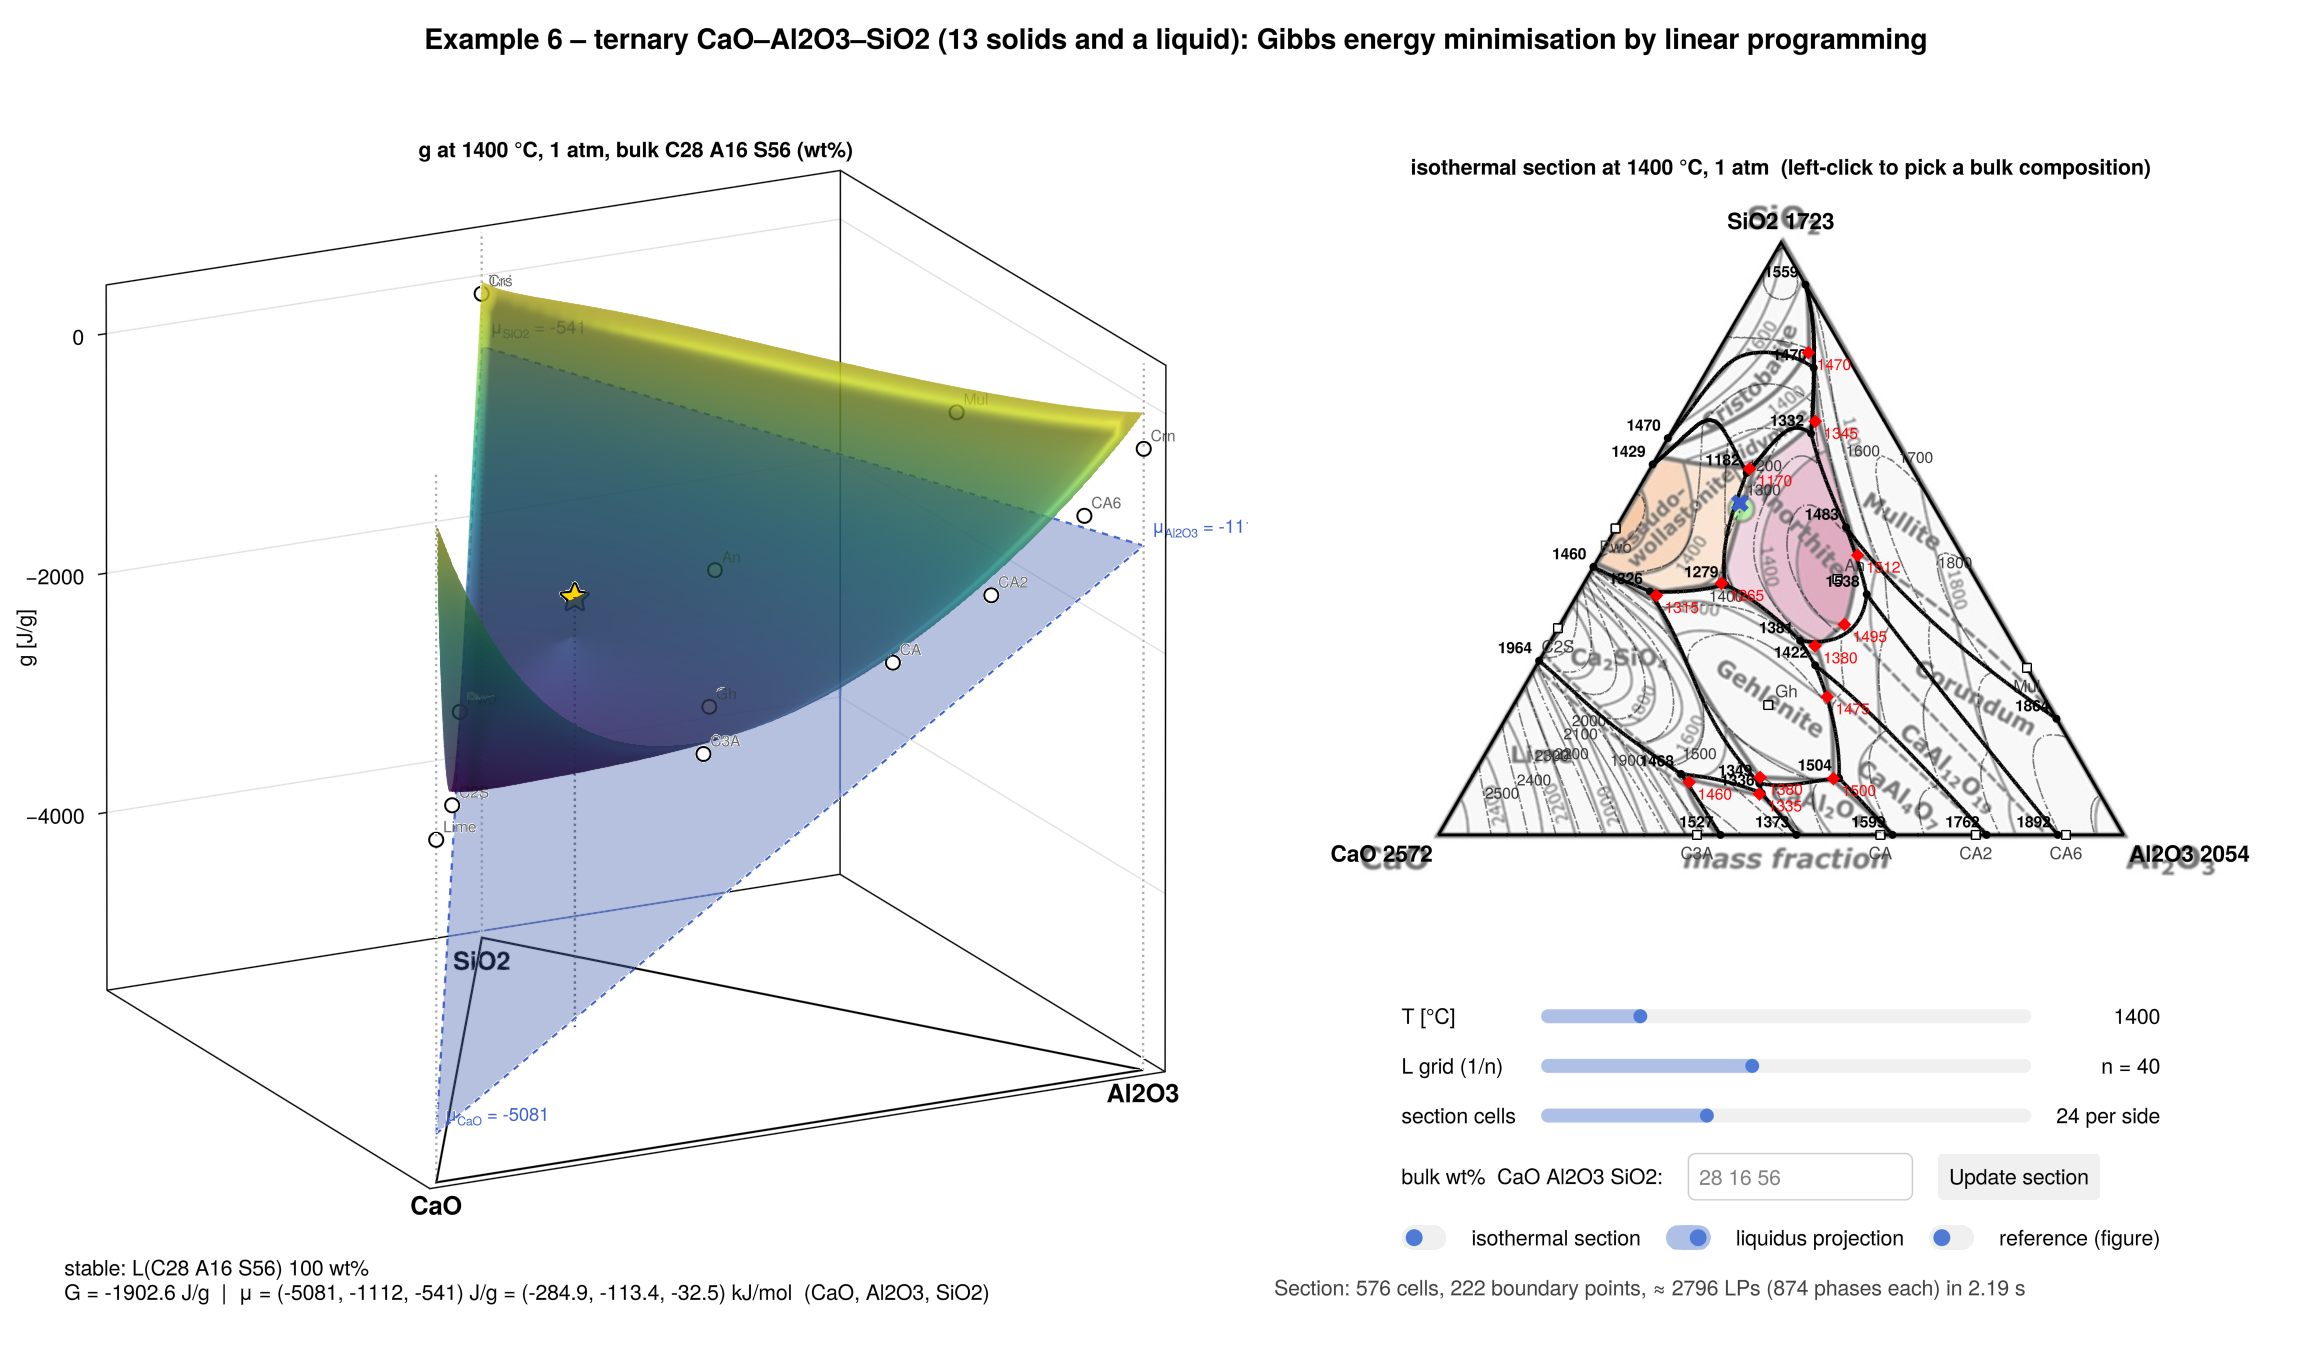
\includegraphics[width=0.49\textwidth]{figures/ex6_reference.png}\hfill
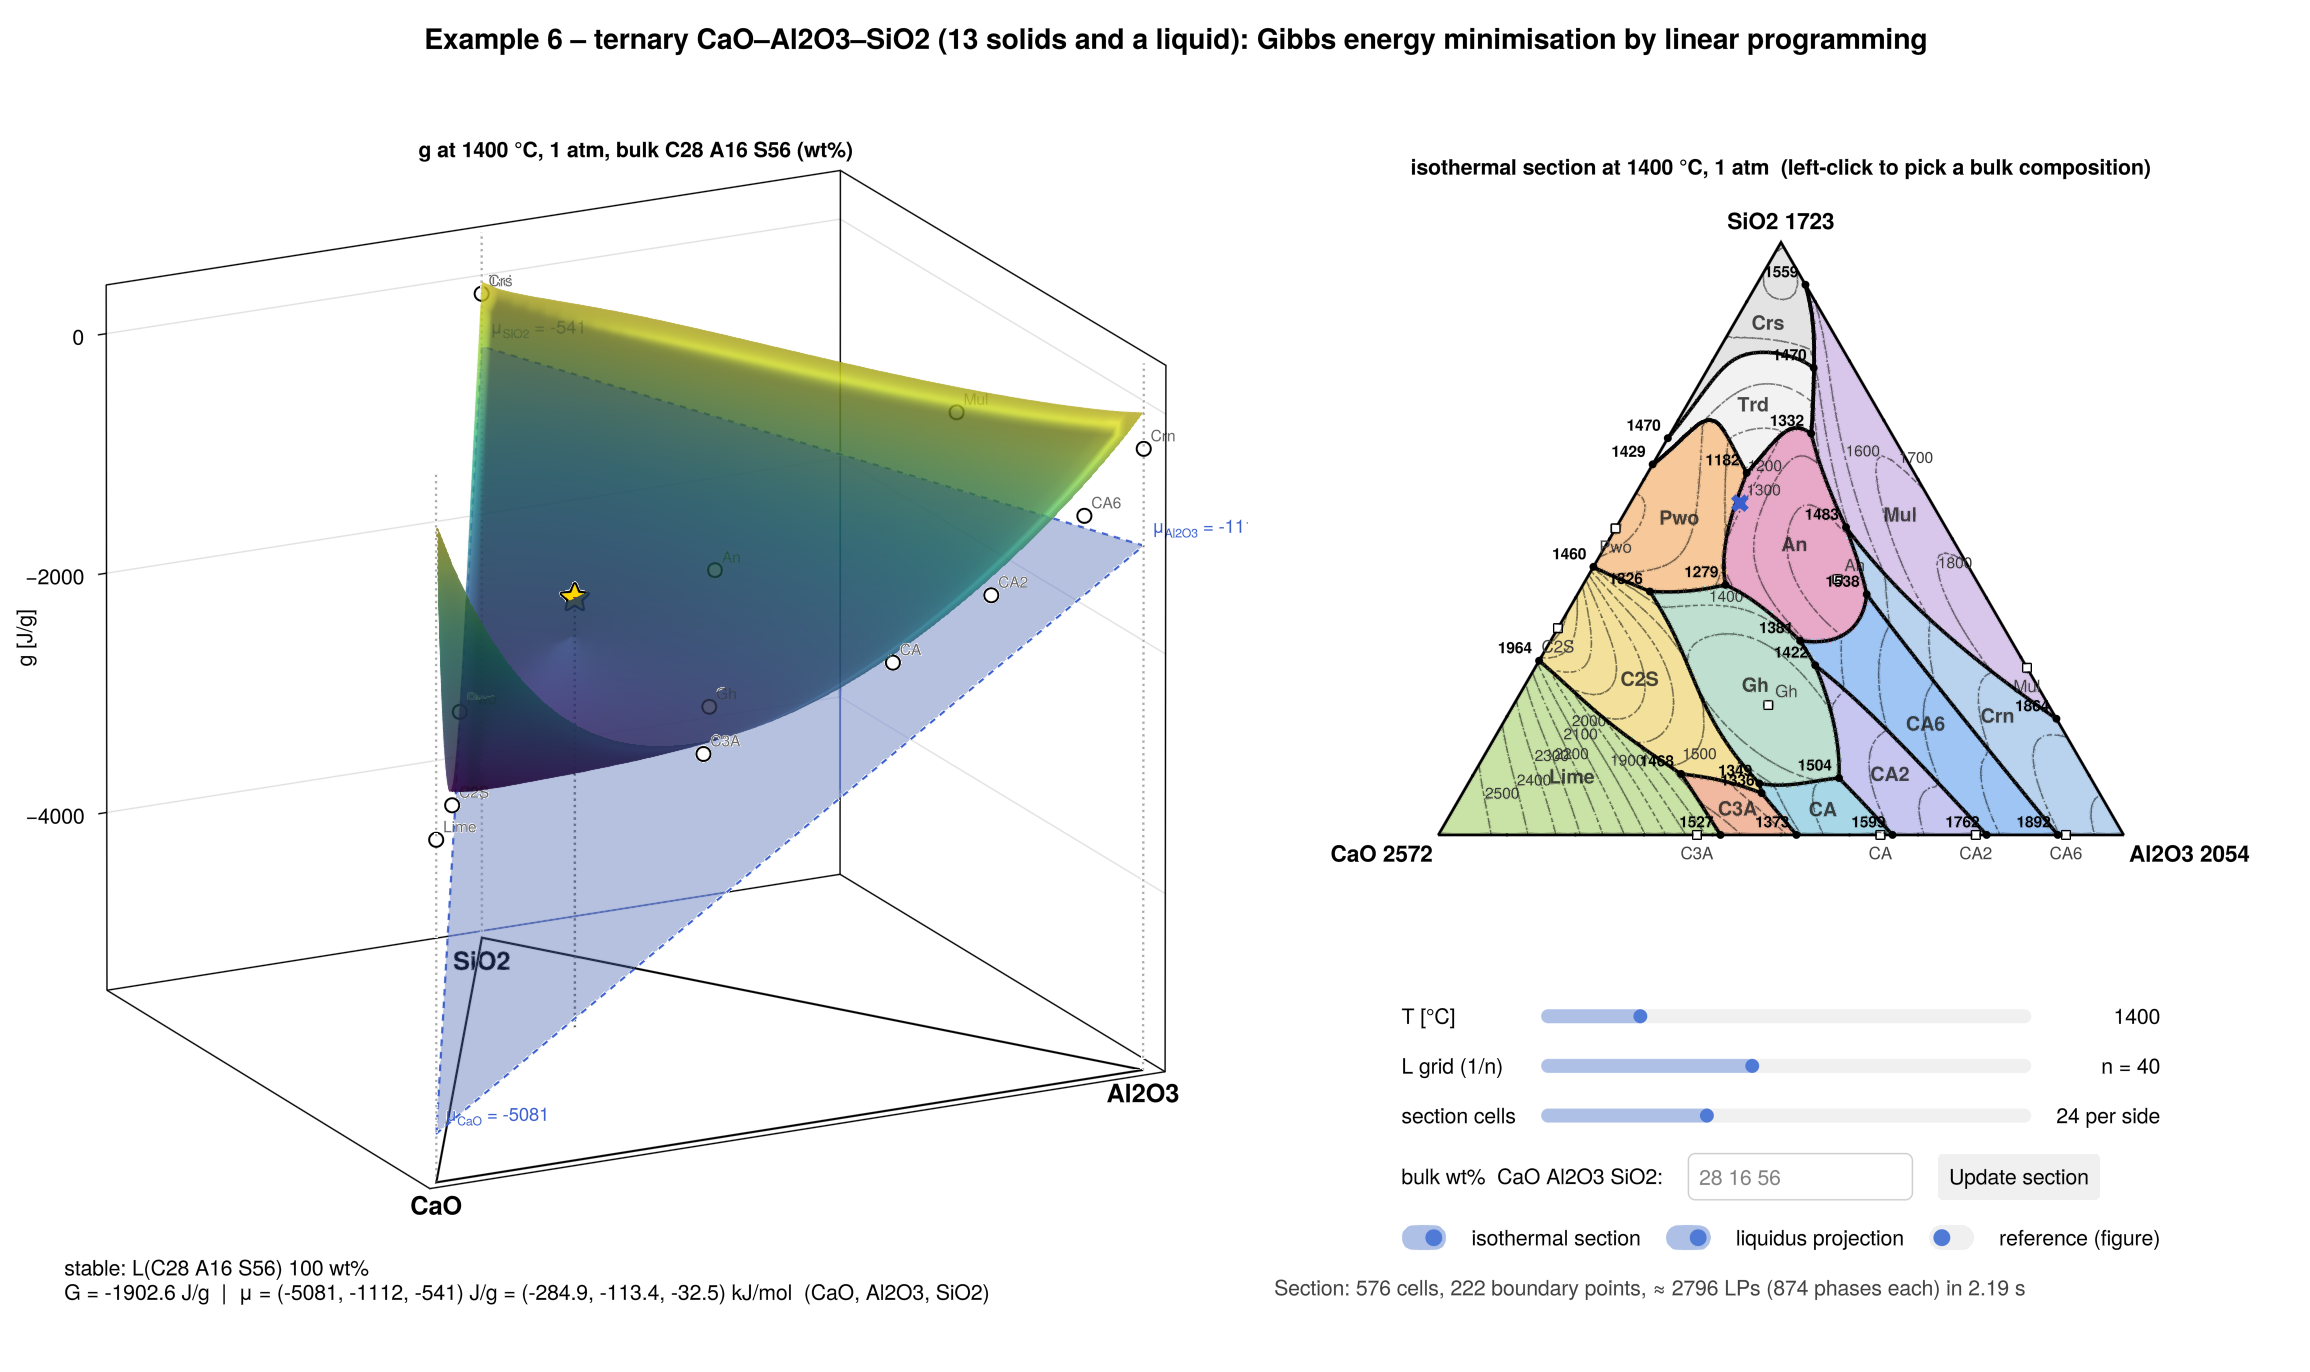
\includegraphics[width=0.49\textwidth]{figures/ex6_projection.png}
\caption{Left: the liquidus projection of the model drawn over the course figure (\ctl{reference (figure)}
on, isothermal section off); red diamonds: invariant points used for the calibration with their literature
temperatures, black: the model. Right: the liquidus projection of the model alone, coloured by primary field.}
\end{figure}

\begin{figure}[H]
\centering
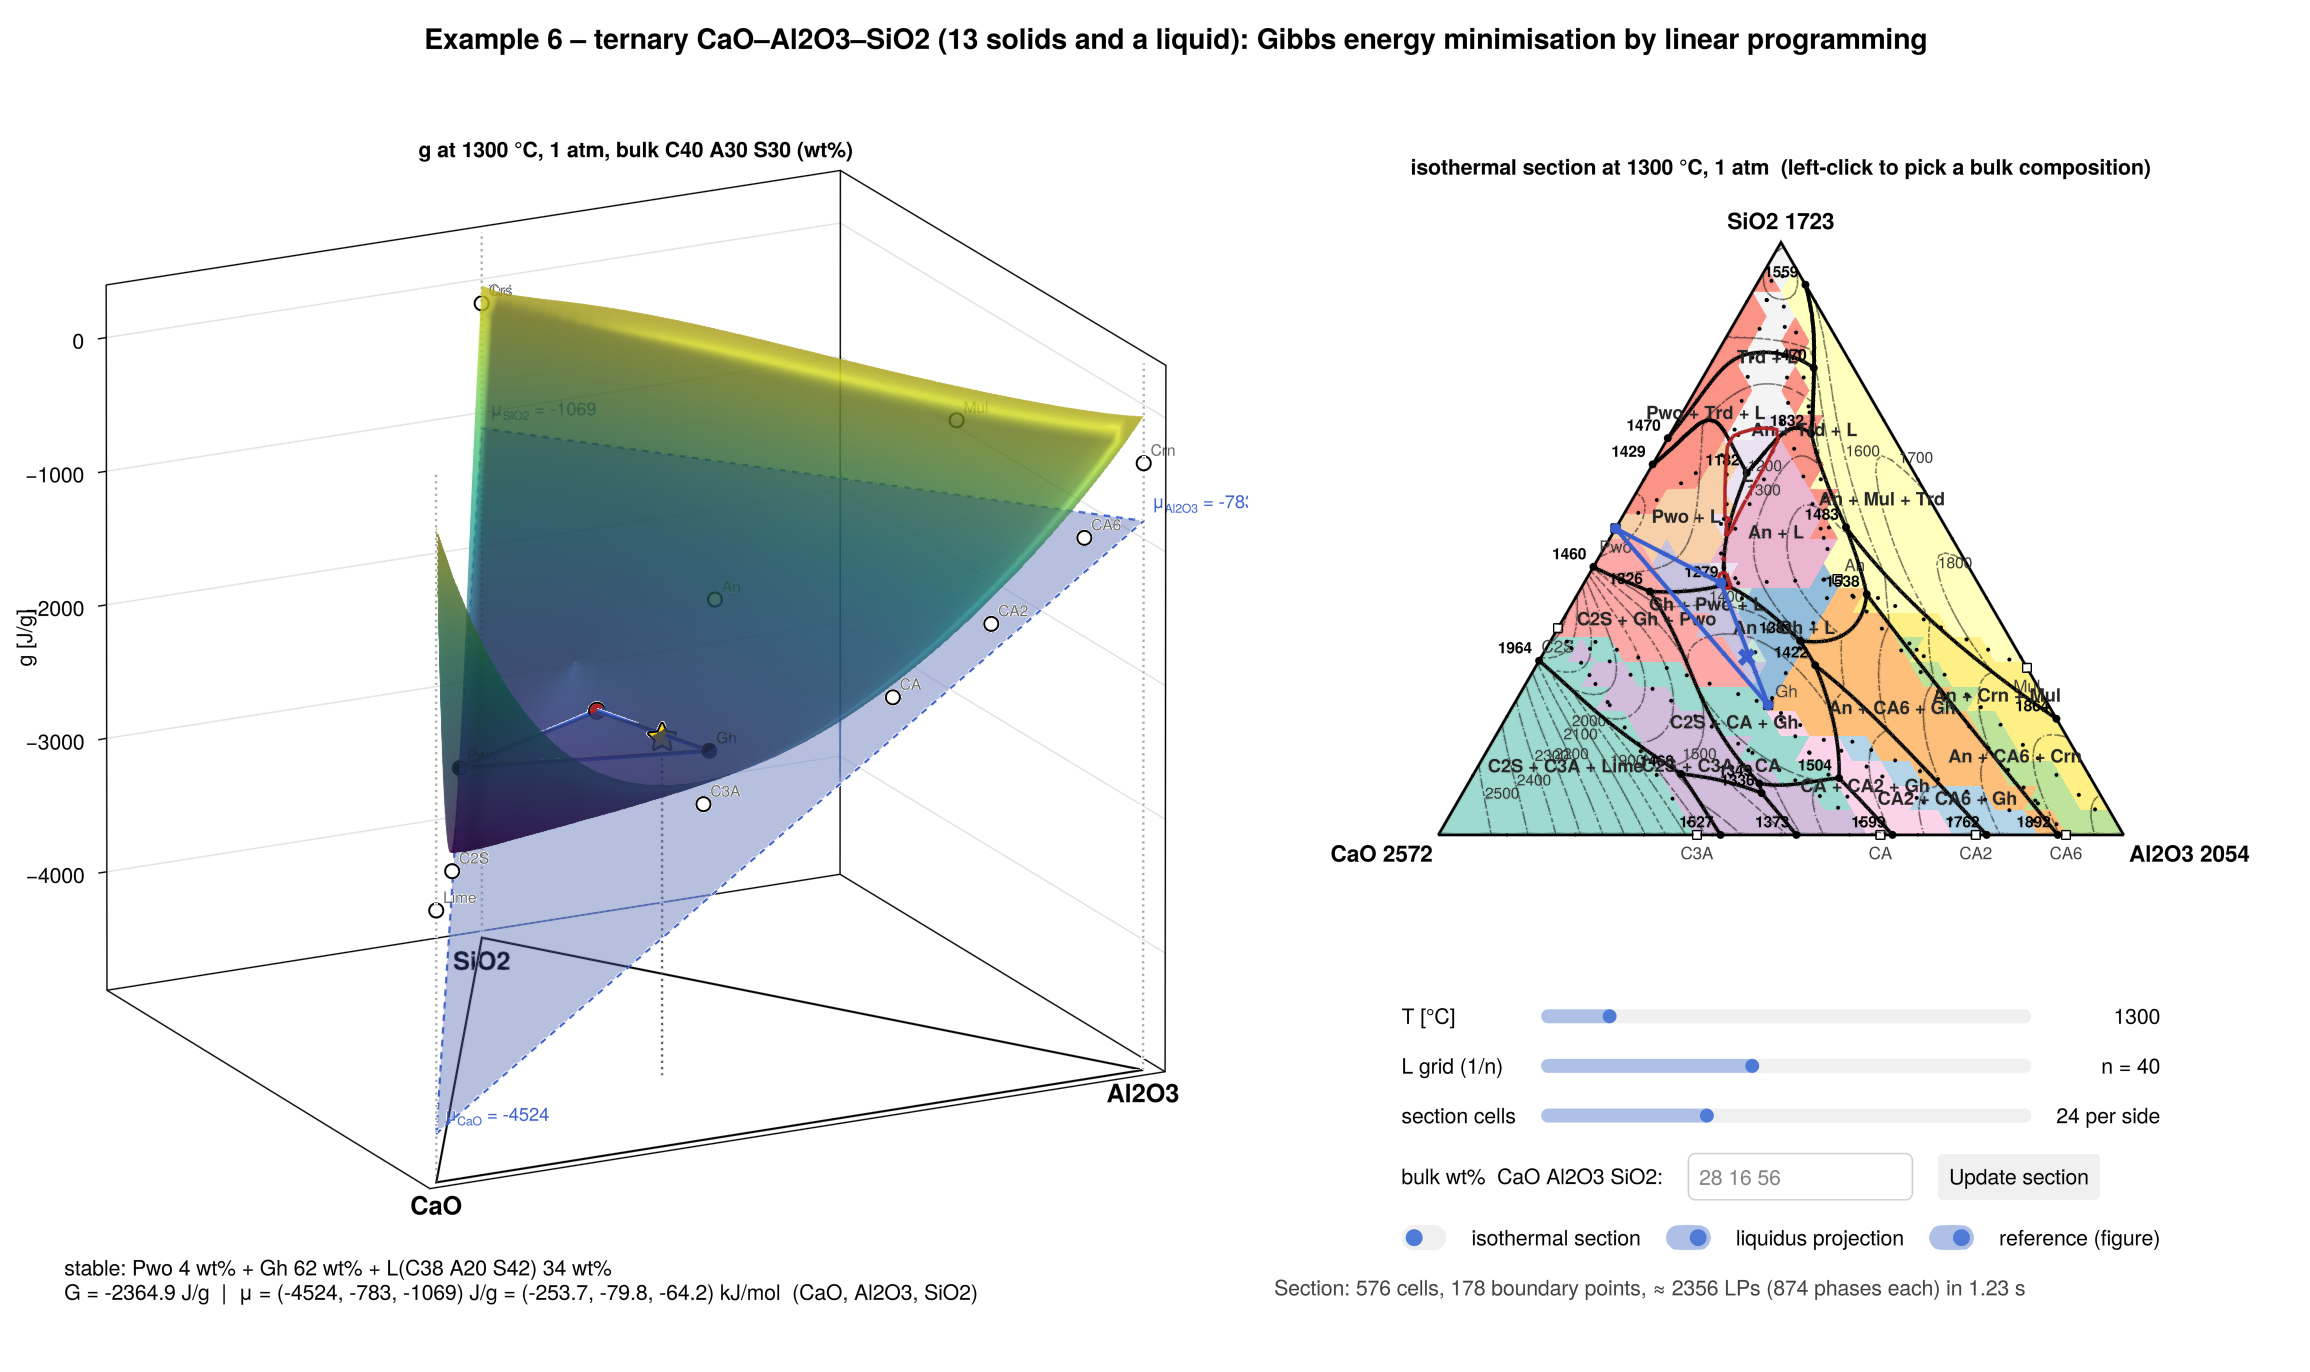
\includegraphics[width=0.75\textwidth]{figures/ex6_1300.png}
\caption{1300\,$^\circ$C, bulk C40 A30 S30: Pwo + Gh + L (a three-phase triangle). The tangent plane touches
the two solids and the liquid.}
\end{figure}

\begin{tryit}
\begin{itemize}
\item Cool the green dot C28 A16 S56 from 1400\,$^\circ$C. At which temperature does the first solid appear,
  and which one? The composition lies on the Pwo–An boundary: what crystallises together, and where does the
  liquid go? Below which temperature is everything solid (An + Pwo + Trd)?
\item Heat the anorthite composition (C20 A37 S43) through 1553\,$^\circ$C and then the CA6 composition
  (C8 A92 S0) through about 1890\,$^\circ$C. Which one melts to a liquid of its own composition, and what does
  the other one give?
\item Switch on \ctl{reference (figure)} with the isothermal section off. Where does the model differ most
  from the figure? Explain the difference near the SiO$_2$ corner with Example~3.
\item At 1300\,$^\circ$C find the three-phase triangles. Each solid–solid side of a triangle is an
  \emph{Alkemade line}; which compounds are joined in this way?
\item In the 3D view, compare the dot of a solid with the liquid surface directly above or below it: below
  the melting point the solid lies below the liquid of the same composition, Eq.~\eqref{eq:cassol}.
\end{itemize}
\end{tryit}

%==============================================================================
\clearpage
\section{Troubleshooting}
%==============================================================================
\begin{itemize}
\item \textbf{``Package … not found''}: run the installation command of Section~\ref{sec:intro} again in the
  main folder.
\item \textbf{The first start is slow}: normal (compilation). Keep the REPL open and \lstinline{include} the next
  example in the same session — but note that two examples cannot be loaded into the \emph{same} session one
  after the other, because they define the same names; restart Julia in between.
\item \textbf{The program reacts slowly}: reduce the number of pseudocompounds or grid nodes / section cells.
\item \textbf{The window is too large for the screen}: reduce \lstinline{WINDOW_FRACTION} in
  \file{window\_size.jl}, e.g.\ to \lstinline{(0.7, 0.7)}, and start the program again.
\item \textbf{``not possible''} (Example 1): the active phases cannot make the chosen bulk composition, e.g.\ only
  A2B and AB2 are switched on and $X_B < 1/3$.
\item \textbf{Changed data have no effect}: the USER INPUT block is read when the program starts; save the file
  and start the program again.
\item \textbf{New screenshots for this guide}: \lstinline{julia guide/make_screenshots.jl all}, then compile
  \file{guide/guide.tex}.
\end{itemize}

\end{document}
